% Options for packages loaded elsewhere
\PassOptionsToPackage{unicode}{hyperref}
\PassOptionsToPackage{hyphens}{url}
%
\documentclass[
  12pt,
]{book}
\usepackage{amsmath,amssymb}
\usepackage{lmodern}
\usepackage{iftex}
\ifPDFTeX
  \usepackage[T1]{fontenc}
  \usepackage[utf8]{inputenc}
  \usepackage{textcomp} % provide euro and other symbols
\else % if luatex or xetex
  \usepackage{unicode-math}
  \defaultfontfeatures{Scale=MatchLowercase}
  \defaultfontfeatures[\rmfamily]{Ligatures=TeX,Scale=1}
\fi
% Use upquote if available, for straight quotes in verbatim environments
\IfFileExists{upquote.sty}{\usepackage{upquote}}{}
\IfFileExists{microtype.sty}{% use microtype if available
  \usepackage[]{microtype}
  \UseMicrotypeSet[protrusion]{basicmath} % disable protrusion for tt fonts
}{}
\makeatletter
\@ifundefined{KOMAClassName}{% if non-KOMA class
  \IfFileExists{parskip.sty}{%
    \usepackage{parskip}
  }{% else
    \setlength{\parindent}{0pt}
    \setlength{\parskip}{6pt plus 2pt minus 1pt}}
}{% if KOMA class
  \KOMAoptions{parskip=half}}
\makeatother
\usepackage{xcolor}
\usepackage{color}
\usepackage{fancyvrb}
\newcommand{\VerbBar}{|}
\newcommand{\VERB}{\Verb[commandchars=\\\{\}]}
\DefineVerbatimEnvironment{Highlighting}{Verbatim}{commandchars=\\\{\}}
% Add ',fontsize=\small' for more characters per line
\usepackage{framed}
\definecolor{shadecolor}{RGB}{248,248,248}
\newenvironment{Shaded}{\begin{snugshade}}{\end{snugshade}}
\newcommand{\AlertTok}[1]{\textcolor[rgb]{0.94,0.16,0.16}{#1}}
\newcommand{\AnnotationTok}[1]{\textcolor[rgb]{0.56,0.35,0.01}{\textbf{\textit{#1}}}}
\newcommand{\AttributeTok}[1]{\textcolor[rgb]{0.77,0.63,0.00}{#1}}
\newcommand{\BaseNTok}[1]{\textcolor[rgb]{0.00,0.00,0.81}{#1}}
\newcommand{\BuiltInTok}[1]{#1}
\newcommand{\CharTok}[1]{\textcolor[rgb]{0.31,0.60,0.02}{#1}}
\newcommand{\CommentTok}[1]{\textcolor[rgb]{0.56,0.35,0.01}{\textit{#1}}}
\newcommand{\CommentVarTok}[1]{\textcolor[rgb]{0.56,0.35,0.01}{\textbf{\textit{#1}}}}
\newcommand{\ConstantTok}[1]{\textcolor[rgb]{0.00,0.00,0.00}{#1}}
\newcommand{\ControlFlowTok}[1]{\textcolor[rgb]{0.13,0.29,0.53}{\textbf{#1}}}
\newcommand{\DataTypeTok}[1]{\textcolor[rgb]{0.13,0.29,0.53}{#1}}
\newcommand{\DecValTok}[1]{\textcolor[rgb]{0.00,0.00,0.81}{#1}}
\newcommand{\DocumentationTok}[1]{\textcolor[rgb]{0.56,0.35,0.01}{\textbf{\textit{#1}}}}
\newcommand{\ErrorTok}[1]{\textcolor[rgb]{0.64,0.00,0.00}{\textbf{#1}}}
\newcommand{\ExtensionTok}[1]{#1}
\newcommand{\FloatTok}[1]{\textcolor[rgb]{0.00,0.00,0.81}{#1}}
\newcommand{\FunctionTok}[1]{\textcolor[rgb]{0.00,0.00,0.00}{#1}}
\newcommand{\ImportTok}[1]{#1}
\newcommand{\InformationTok}[1]{\textcolor[rgb]{0.56,0.35,0.01}{\textbf{\textit{#1}}}}
\newcommand{\KeywordTok}[1]{\textcolor[rgb]{0.13,0.29,0.53}{\textbf{#1}}}
\newcommand{\NormalTok}[1]{#1}
\newcommand{\OperatorTok}[1]{\textcolor[rgb]{0.81,0.36,0.00}{\textbf{#1}}}
\newcommand{\OtherTok}[1]{\textcolor[rgb]{0.56,0.35,0.01}{#1}}
\newcommand{\PreprocessorTok}[1]{\textcolor[rgb]{0.56,0.35,0.01}{\textit{#1}}}
\newcommand{\RegionMarkerTok}[1]{#1}
\newcommand{\SpecialCharTok}[1]{\textcolor[rgb]{0.00,0.00,0.00}{#1}}
\newcommand{\SpecialStringTok}[1]{\textcolor[rgb]{0.31,0.60,0.02}{#1}}
\newcommand{\StringTok}[1]{\textcolor[rgb]{0.31,0.60,0.02}{#1}}
\newcommand{\VariableTok}[1]{\textcolor[rgb]{0.00,0.00,0.00}{#1}}
\newcommand{\VerbatimStringTok}[1]{\textcolor[rgb]{0.31,0.60,0.02}{#1}}
\newcommand{\WarningTok}[1]{\textcolor[rgb]{0.56,0.35,0.01}{\textbf{\textit{#1}}}}
\usepackage{longtable,booktabs,array}
\usepackage{calc} % for calculating minipage widths
% Correct order of tables after \paragraph or \subparagraph
\usepackage{etoolbox}
\makeatletter
\patchcmd\longtable{\par}{\if@noskipsec\mbox{}\fi\par}{}{}
\makeatother
% Allow footnotes in longtable head/foot
\IfFileExists{footnotehyper.sty}{\usepackage{footnotehyper}}{\usepackage{footnote}}
\makesavenoteenv{longtable}
\usepackage{graphicx}
\makeatletter
\def\maxwidth{\ifdim\Gin@nat@width>\linewidth\linewidth\else\Gin@nat@width\fi}
\def\maxheight{\ifdim\Gin@nat@height>\textheight\textheight\else\Gin@nat@height\fi}
\makeatother
% Scale images if necessary, so that they will not overflow the page
% margins by default, and it is still possible to overwrite the defaults
% using explicit options in \includegraphics[width, height, ...]{}
\setkeys{Gin}{width=\maxwidth,height=\maxheight,keepaspectratio}
% Set default figure placement to htbp
\makeatletter
\def\fps@figure{htbp}
\makeatother
\setlength{\emergencystretch}{3em} % prevent overfull lines
\providecommand{\tightlist}{%
  \setlength{\itemsep}{0pt}\setlength{\parskip}{0pt}}
\setcounter{secnumdepth}{5}
\usepackage{booktabs}
\usepackage{longtable}
\usepackage[bf,singlelinecheck=on]{caption}

\usepackage[bookmarksnumbered]{hyperref}
\hypersetup{bookmarksnumbered=true}

\usepackage[BoldFont,SlantFont,CJKchecksingle]{xeCJK}
\setCJKmonofont{SimSun}% 设置缺省中文字体
%\parindent 2em   %段首缩进

\usepackage[
  top=1cm,
  bottom=1cm,
  left=3cm,
  right=2cm,
  headheight=30pt, % as per the warning by fancyhdr
  includehead,includefoot,
  heightrounded, % to avoid spurious underfull messages
]{geometry}

\usepackage[heading]{ctex}

\setlength{\parindent}{2em}

\usepackage{fancyhdr}
\pagestyle{fancy}
\fancyhead[LO]{
\includegraphics[width=4cm]{./img/logo_en.jpg}}
\fancyhead[RE]{
\includegraphics[width=4cm]{./img/logo_en.jpg}}
%\rhead{\bfseries Result}


%\setmainfont[UprightFeatures={SmallCapsFont=AlegreyaSC-Regular}]{Alegreya}
%\setmainfont[]{Alegreya}
\setmainfont{Times New Roman}
\setmonofont[Scale=MatchLowercase]{Source Code Pro}
\setmonofont[Scale=0.8]{Source Code Pro}

\usepackage{framed,color}
\definecolor{shadecolor}{RGB}{248,248,248}

\renewcommand{\textfraction}{0.05}
\renewcommand{\topfraction}{0.8}
\renewcommand{\bottomfraction}{0.8}
\renewcommand{\floatpagefraction}{0.75}

\renewenvironment{quote}{\begin{VF}}{\end{VF}}
\let\oldhref\href
\renewcommand{\href}[2]{#2\footnote{\url{#1}}}

\ifxetex
  \usepackage{letltxmacro}
  \setlength{\XeTeXLinkMargin}{1pt}
  \LetLtxMacro\SavedIncludeGraphics\includegraphics
  \def\includegraphics#1#{% #1 catches optional stuff (star/opt. arg.)
    \IncludeGraphicsAux{#1}%
  }%
  \newcommand*{\IncludeGraphicsAux}[2]{%
    \XeTeXLinkBox{%
      \SavedIncludeGraphics#1{#2}%
    }%
  }%
\fi

\makeatletter
\newenvironment{kframe}{%
\medskip{}
\setlength{\fboxsep}{.8em}
 \def\at@end@of@kframe{}%
 \ifinner\ifhmode%
  \def\at@end@of@kframe{\end{minipage}}%
  \begin{minipage}{\columnwidth}%
 \fi\fi%
 \def\FrameCommand##1{\hskip\@totalleftmargin \hskip-\fboxsep
 \colorbox{shadecolor}{##1}\hskip-\fboxsep
     % There is no \\@totalrightmargin, so:
     \hskip-\linewidth \hskip-\@totalleftmargin \hskip\columnwidth}%
 \MakeFramed {\advance\hsize-\width
   \@totalleftmargin\z@ \linewidth\hsize
   \@setminipage}}%
 {\par\unskip\endMakeFramed%
 \at@end@of@kframe}
\makeatother

\makeatletter
\@ifundefined{Shaded}{
}{\renewenvironment{Shaded}{\begin{kframe}}{\end{kframe}}}
\makeatother

\newenvironment{rmdblock}[1]
  {
  \begin{itemize}
  \renewcommand{\labelitemi}{
    \raisebox{-.7\height}[0pt][0pt]{
      {\setkeys{Gin}{width=3em,keepaspectratio}\includegraphics{images/#1}}
    }
  }
  \setlength{\fboxsep}{1em}
  \begin{kframe}
  \item
  }
  {
  \end{kframe}
  \end{itemize}
  }
\newenvironment{rmdnote}
  {\begin{rmdblock}{note}}
  {\end{rmdblock}}
\newenvironment{rmdcaution}
  {\begin{rmdblock}{caution}}
  {\end{rmdblock}}
\newenvironment{rmdimportant}
  {\begin{rmdblock}{important}}
  {\end{rmdblock}}
\newenvironment{rmdtip}
  {\begin{rmdblock}{tip}}
  {\end{rmdblock}}
\newenvironment{rmdwarning}
  {\begin{rmdblock}{warning}}
  {\end{rmdblock}}

\usepackage{makeidx}
\makeindex

\urlstyle{tt}

\usepackage{amsthm}
\makeatletter
\def\thm@space@setup{%
  \thm@preskip=8pt plus 2pt minus 4pt
  \thm@postskip=\thm@preskip
}
\makeatother

\frontmatter

\let\oldmaketitle\maketitle
\AtBeginDocument{\let\maketitle\relax}

% % Definition of \maketitle
% \makeatletter
%     \begin{titlepage}
%         \begin{center}
%             
\includegraphics[width=0.7\linewidth]{./img/logo_en.jpg}\\[4ex]
%             {\huge \bfseries  \@title }\\[2ex]
%             {\LARGE  \@author}\\[50ex]
%             {\large \@date}
%         \end{center}
%     \end{titlepage}
% \makeatother

\ifLuaTeX
  \usepackage{selnolig}  % disable illegal ligatures
\fi
\usepackage[]{natbib}
\bibliographystyle{apalike}
\IfFileExists{bookmark.sty}{\usepackage{bookmark}}{\usepackage{hyperref}}
\IfFileExists{xurl.sty}{\usepackage{xurl}}{} % add URL line breaks if available
\urlstyle{same} % disable monospaced font for URLs
\hypersetup{
  pdftitle={低功耗蓝牙开发者手册},
  pdfauthor={Ingchips Technology Co., Ltd.},
  hidelinks,
  pdfcreator={LaTeX via pandoc}}

\title{低功耗蓝牙开发者手册}
\author{Ingchips Technology Co., Ltd.}
\date{}

\begin{document}
\maketitle

%\cleardoublepage\newpage\thispagestyle{empty}\null
%\cleardoublepage\newpage\thispagestyle{empty}\null
%\cleardoublepage\newpage
\thispagestyle{empty}
\begin{center}
\end{center}

\setlength{\abovedisplayskip}{-5pt}
\setlength{\abovedisplayshortskip}{-5pt}

\thispagestyle{empty}

\makeatletter
\begin{center}
    \vspace{5ex}
    
\includegraphics{./img/logo_en.jpg}\\[15ex]
    {\huge  \@title }
    \vspace{48ex}
\end{center}

桃芯科技(苏州)有限公司

官网:www.ingchips.com

邮箱:service@ingchips.com

电话:010-85160285

地址:北京市海淀区知春路 49 号紫金数 3 号楼 8 层 803

\hspace{2.8em}上海市浦东新区祥科路58号炬芯大厦A座3层316

\hspace{2.8em}深圳市南山区科技园曙光大厦1009

\makeatother

\newpage
\thispagestyle{empty}

\makeatletter

\vspace*{40em}

\emph{版权申明}

本文档以及其所包含的内容为桃芯科技(苏州)有限公司所有,并受中国法律和其他可适用的国际公约的版权保护。
未经桃芯科技的事先书面许可,不得在任何其他地方以任何形式(有形或无形的)以任何电子或其他方式复制、
分发、传输、展示、出版或广播,不允许从内容的任何副本中更改或删除任何商标、版权或其他通知。
违反者将对其违反行为所造成的任何以及全部损害承担责任, 桃芯科技保留采取任何法律所允许范围内救济措施的权利。

%\let\maketitle\oldmaketitle
%\maketitle

{
\setcounter{tocdepth}{2}
\tableofcontents
}
\listoffigures
\listoftables
\hypertarget{revision-history}{%
\chapter{版本历史}\label{revision-history}}

\begin{longtable}[]{@{}
  >{\centering\arraybackslash}p{(\columnwidth - 4\tabcolsep) * \real{0.1270}}
  >{\raggedright\arraybackslash}p{(\columnwidth - 4\tabcolsep) * \real{0.7143}}
  >{\centering\arraybackslash}p{(\columnwidth - 4\tabcolsep) * \real{0.1587}}@{}}
\toprule()
\begin{minipage}[b]{\linewidth}\centering
版本
\end{minipage} & \begin{minipage}[b]{\linewidth}\raggedright
信息
\end{minipage} & \begin{minipage}[b]{\linewidth}\centering
日期
\end{minipage} \\
\midrule()
\endhead
0.5 & 初始版本 & 2022-09-07 \\
0.6 & 增加减速模式、功率控制 & 2022-09-15 \\
0.6.1 & 修正拼写错误等 & 2022-09-28 \\
0.7 & 针对 SDK v8.2 更新 & 2022-10-31 \\
0.8 & 增加同步版 API、线程安全 API 等 & 2022-11-19 \\
0.9 & 增加 L2CAP 基于信用点的连接 & 2023-01-17 \\
0.9.1 & 更新 SM 说明 & 2023-01-30 \\
0.9.2 & 更新协议栈能力 & 2023-02-11 \\
0.9.3 & 增加``非标''扩展 & 2023-02-20 \\
0.9.4 & 增加``特性简析'' & 2023-03-22 \\
0.9.5 & 增加``加密与解密'' & 2023-04-07 \\
0.9.6 & 更新 ING916 协议栈能力 & 2023-04-26 \\
0.9.7 & 更新 ING916 协议栈能力 & 2023-06-21 \\
0.9.8 & 增加 PAwR 相关内容 & 2023-11-06 \\
\bottomrule()
\end{longtable}

\mainmatter

\hypertarget{ch-intro}{%
\chapter{简介}\label{ch-intro}}

欢迎使用 \emph{INGCHIPS} 918XX/916XX 软件开发工具包 (SDK).

本手册将带您了解 \emph{INGCHIPS} 各系列 BLE SoC 芯片上的低功耗蓝牙开发,了解整个协议栈设计思路,
熟悉各模块主要接口的使用方法。

本手册侧重从开发者的角度介绍 BLE 的开发,涉及 BLE 规范时采用了更``实用化''的描述,
不去关注规范里的每一个细节。

SDK 工具可以生成本手册里提到的一些常见代码,如回调函数、事件处理等。

\hypertarget{ux7f29ux7565ux8bedux53caux672fux8bed}{%
\section{缩略语及术语}\label{ux7f29ux7565ux8bedux53caux672fux8bed}}

\begin{longtable}[]{@{}ll@{}}
\caption{\label{tab:ch0-abbreviations} 缩略语}\tabularnewline
\toprule()
缩略语 & 说明 \\
\midrule()
\endfirsthead
\toprule()
缩略语 & 说明 \\
\midrule()
\endhead
BLE & 低功耗蓝牙(Bluetooth LE,Bluetooth Low Engergy) \\
CCCD & 客户端特征配置描述符(Client Characteristic Configuration Descriptor) \\
CTE & 定频扩展(Constant Tone Extension) \\
HCI & Host Controller 接口 \\
L2CAP & 逻辑链路控制与适配协议(Logical Link Control and Adaptation Protocol) \\
LL & 链路层(Link Layer) \\
LMP & BR/EDR 的链路管理协议(Link Manager Protocol) \\
LTK & 长期密钥(Long Term Key) \\
MIC & 消息认证码(Message Integrity Code) \\
MITM & 中间人(Man-In-The-Middle) \\
RSSI & 接收信号强度指示(Received Signal Strength Indicator) \\
SCA & 睡眠时钟精度(Sleep Clock Accuracy) \\
SPSM & 简化的协议/服务选择器(Simplified Protocol/Service Multiplexer) \\
UUID & 通用唯一识别码(Universally Unique IDentifier) \\
\bottomrule()
\end{longtable}

\begin{longtable}[]{@{}ll@{}}
\caption{\label{tab:ch0-term} 术语}\tabularnewline
\toprule()
术语 & 说明 \\
\midrule()
\endfirsthead
\toprule()
术语 & 说明 \\
\midrule()
\endhead
1M & BLE 使用的一种 PHY,符号速率为 \(1Msps\) \\
2M & BLE 使用的一种 PHY,符号速率为 \(2Msps\) \\
Characteristic & 特征,是服务的组成部分 \\
Coded & BLE 使用的一种 PHY,基于卷积码的信道编码 \\
Controller & BLE 控制器,整个蓝牙协议栈偏低层的部分 \\
Handle & 句柄 \\
Host & BLE 主机,整个蓝牙协议栈偏上层的部分 \\
PHY & BLE 的物理层传输方式 \\
Service & 服务,由特征组成 \\
\bottomrule()
\end{longtable}

蓝牙规范从 v5.3 版本开始更新了部分术语,本手册沿用旧称。表 \ref{tab:ch0-new-term} 是这部分术语的新旧对照。

\begin{longtable}[]{@{}lll@{}}
\caption{\label{tab:ch0-new-term} 新旧术语对照}\tabularnewline
\toprule()
原名称 & 新名称 & 本手册 \\
\midrule()
\endfirsthead
\toprule()
原名称 & 新名称 & 本手册 \\
\midrule()
\endhead
Master & Central & 主角色 \\
Slave & Peripheral & 从角色 \\
White List & Accept List & 白名单 \\
\bottomrule()
\end{longtable}

\hypertarget{ux53c2ux8003ux6587ux6863}{%
\section{参考文档}\label{ux53c2ux8003ux6587ux6863}}

\begin{enumerate}
\def\labelenumi{\arabic{enumi}.}
\tightlist
\item
  Bluetooth SIG\footnote{\url{https://www.bluetooth.com/}}
\item
  Controller API Reference
\item
  Application Note: Direction Finding Solution\footnote{\url{https://ingchips.github.io/application-notes/an_aoa/index.html}}
\end{enumerate}

\hypertarget{ch-overview}{%
\chapter{概览}\label{ch-overview}}

\hypertarget{ux57faux672cux539fux5219}{%
\section{基本原则}\label{ux57faux672cux539fux5219}}

\begin{enumerate}
\def\labelenumi{\arabic{enumi}.}
\tightlist
\item
  BLE 协议栈\textbf{尽最大努力}执行各项任务,比如

  \begin{itemize}
  \tightlist
  \item
    将发射功率设置为 \(100dBm\),协议栈将以最大功率进行发射
  \item
    广播、连接并发时,部分广播事件、连接事件可能因需要执行其它任务而被忽略(跳过)
  \item
    极端情况下,当协议栈可能会主动终止某些任务并上报相应的事件
  \end{itemize}
\item
  连接模式下已进入 BLE 协议栈的数据包不会丢失、总是可以送达,除非连接断开
\end{enumerate}

\hypertarget{ux534fux8baeux6808ux67b6ux6784}{%
\section{协议栈架构}\label{ux534fux8baeux6808ux67b6ux6784}}

Controller、Host 以两个任务(或者线程)的形式运行,HCI 接口经过特殊设计,尽量减少内存数据的复制。
Host 的架构如图 \ref{fig:ch0-host-overview} 所示,主要通过 GAP、ATT、GATT Client、SM 等 4
个模块为开发者提供操作接口。

\begin{figure}

{\centering 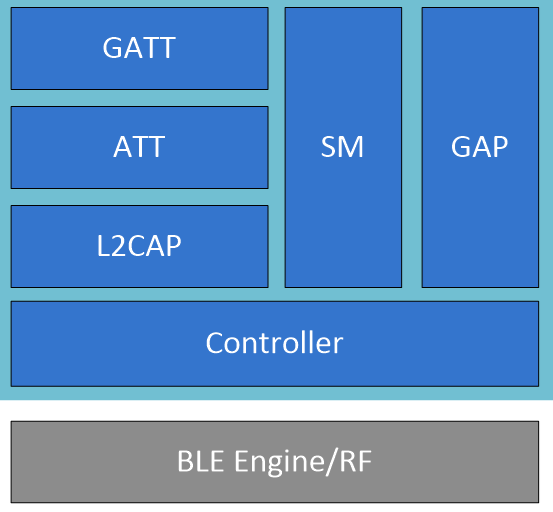
\includegraphics[width=0.5\linewidth]{./img/stack_overview} 

}

\caption{Host 架构}\label{fig:ch0-host-overview}
\end{figure}

Host 任务的伪代码如下:

\begin{Shaded}
\begin{Highlighting}[]
\DataTypeTok{void}\NormalTok{ host\_task}\OperatorTok{(}\DataTypeTok{void}\OperatorTok{)}
\OperatorTok{\{}
\NormalTok{    host\_init}\OperatorTok{();}
    \ControlFlowTok{while} \OperatorTok{(}\NormalTok{true}\OperatorTok{)}
    \OperatorTok{\{}
        \ControlFlowTok{if} \OperatorTok{(}\NormalTok{recv\_msg}\OperatorTok{(}\NormalTok{msg}\OperatorTok{)} \OperatorTok{!=} \DecValTok{0}\OperatorTok{)} \ControlFlowTok{continue}\OperatorTok{;}
\NormalTok{        process\_msg}\OperatorTok{(}\NormalTok{msg}\OperatorTok{);}
    \OperatorTok{\}}
\OperatorTok{\}}
\end{Highlighting}
\end{Shaded}

也就是说 Host 任务是由各种消息驱动的。这些消息既包括来自 Controller 的事件、ACL 数据,
也包含软件定时器消息和用户发送的消息(\texttt{btstack\_push\_user\_msg} 和 \texttt{btstack\_push\_user\_runnable})。

\texttt{process\_msg} 的伪代码如下:

\begin{Shaded}
\begin{Highlighting}[]
\DataTypeTok{void}\NormalTok{ process\_msg}\OperatorTok{(}\NormalTok{msg}\OperatorTok{)}
\OperatorTok{\{}
    \ControlFlowTok{switch} \OperatorTok{(}\NormalTok{msg}\OperatorTok{)}
    \OperatorTok{\{}
    \ControlFlowTok{case}\NormalTok{ HCI Event}\OperatorTok{:}
\NormalTok{        调用各个回调}\OperatorTok{();}
        \ControlFlowTok{break}\OperatorTok{;}
    \ControlFlowTok{case}\NormalTok{ ACL 数据}\OperatorTok{:}
\NormalTok{        调用各个回调}\OperatorTok{();}
        \ControlFlowTok{break}\OperatorTok{;}
    \ControlFlowTok{case}\NormalTok{ 软件定时器}\OperatorTok{:}
\NormalTok{        超时处理}\OperatorTok{();}
        \ControlFlowTok{break}\OperatorTok{;}
    \ControlFlowTok{case}\NormalTok{ 用户消息}\OperatorTok{:}
\NormalTok{        弹出用户消息事件}\OperatorTok{();}
        \ControlFlowTok{break}\OperatorTok{;}
    \ControlFlowTok{case}\NormalTok{ 用户执行体}\OperatorTok{:}
\NormalTok{        运行用户执行体}\OperatorTok{();}
        \ControlFlowTok{break}\OperatorTok{;}
    \OperatorTok{\}}
\OperatorTok{\}}
\end{Highlighting}
\end{Shaded}

各个模块(包含协议内部模块及 App\footnote{如无特殊说明,本文所说的 App 皆指运行在芯片上的蓝牙程序。})通过注册回调函数以响应这些事件。
有的模块在处理这些消息时又会产生其它的新事件,
为了响应这些新事件可以再向这些模块注册回调函数。也就是说,Host 内部各个模块(以及 App)通过消息、回调函数耦合在一起。
例如:

\begin{itemize}
\item
  \texttt{hci\_add\_event\_handler}

  通过这个函数可以注册一个能够监听所有 HCI 事件的回调;
\item
  \texttt{att\_server\_init}

  向 ATT Server 模块注册用以响应特征读写的回调函数。
\end{itemize}

\hypertarget{ch-overview-comm-model}{%
\section{通信模型}\label{ch-overview-comm-model}}

通信是指由一地向另一地进行信息的传输与交换,其目的是传输信息、削减另一地的不确定性。对于 BLE 而言,主要有两种通信方式:
一对多的广播、一对一的连接。低功耗蓝牙定义了四种角色:广播发送方称为广播者(Broadcaster),接收方称为观察者(Observer);
连接的发起方称为主角色(新名称为中心角色,Central),接受方称为从角色(新名称为外围角色,Periperhal)。

蓝牙规范定义了广播数据的格式、AD 类型,见图 \ref{fig:ch0-adv-data-format}。如,AD 类型 \texttt{0x09} 表示设备名称,其后面的 AD 数据域是一个 UTF-8 字符串。
另请参阅``\protect\hyperlink{ch1-adv-data-edit}{广播数据}''一节。

\begin{figure}

{\centering 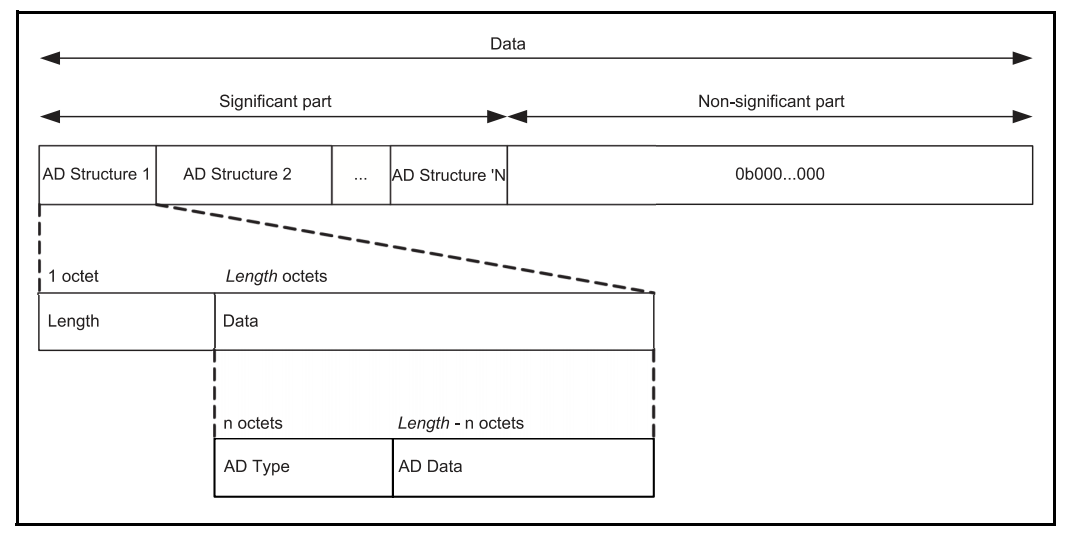
\includegraphics[width=0.8\linewidth]{./img/adv_data_format} 

}

\caption{广播及扫描响应数据包格式}\label{fig:ch0-adv-data-format}
\end{figure}

对于连接模式,低功耗蓝牙定义了特征(Characteristic)和值(Value)这两个概念,进而组织成服务(Service),再由服务组成配置(Profile)。
特征的标识用 UUI\hspace{0pt}D 标识。客户端发现了服务器支持的服务后,就可以读写特征的值,或者订阅特征\footnote{指示服务器端主动报告特征的值。}。
显然特征不见得支持所有这些操作,因此,蓝牙核心规范又为特征定义了属性(Property)、
描述符(Discriptor)等装饰物,以说明特征所支持的操作、需要的权限。UUID 长度为 \(16\) 字节,为了提高传输效率,BLE 定义了一系列特殊的 UUID,
它们的区别仅在于 2 个字节,另外 \(14\) 个字节相同:

\begin{verbatim}
0x0000xxxx-0000-1000-8000-00805F9B34FB
\end{verbatim}

这两个字节就是所谓的 16-bit UUID,由蓝牙特别兴趣小组公司负责管理、分配\footnote{\url{https://www.bluetooth.com/16-bit-uuids-for-sdos/}}。

\hypertarget{ux56deux8c03ux51fdux6570ux4e8bux4ef6ux5305}{%
\section{回调函数事件包}\label{ux56deux8c03ux51fdux6570ux4e8bux4ef6ux5305}}

协议栈的各种回调函数遵循类似的原型,其输入称为事件包:

\begin{Shaded}
\begin{Highlighting}[]
\KeywordTok{typedef} \DataTypeTok{void} \OperatorTok{(*}\NormalTok{btstack\_packet\_handler\_t}\OperatorTok{)} \OperatorTok{(}
    \CommentTok{// 事件包类型}
    \DataTypeTok{uint8\_t}\NormalTok{ packet\_type}\OperatorTok{,}
    \CommentTok{// 关联的信道(一般指蓝牙连接句柄)}
    \DataTypeTok{uint16\_t}\NormalTok{ channel}\OperatorTok{,}
    \CommentTok{// 事件包内容}
    \DataTypeTok{const} \DataTypeTok{uint8\_t} \OperatorTok{*}\NormalTok{packet}\OperatorTok{,}
    \CommentTok{// 事件包内容的长度}
    \DataTypeTok{uint16\_t}\NormalTok{ size}\OperatorTok{);}
\end{Highlighting}
\end{Shaded}

包类型 \texttt{packet\_type} 的取值如下:

\begin{itemize}
\item
  \texttt{HCI\_EVENT\_PACKET}:HCI 事件包(\textbf{常用})

  这个类型的事件包是个``大杂烩'',多个模块弹出的事件包都会使用这个类型。
\item
  \texttt{HCI\_ACL\_DATA\_PACKET}:Controller 上报的 ACL 数据

  这个类型的事件包只会被通过 \texttt{hci\_register\_acl\_packet\_handler} 注册的 ACL 数据回调函数收到。
\item
  \texttt{HCI\_COMPLETED\_SDU\_PACKET}:来自 LE 信用信道的完整 SDU

  这个类型的事件包只会被通过 \texttt{l2cap\_register\_service} 注册的 L2CAP 服务回调函数收到。
\item
  \texttt{L2CAP\_EVENT\_PACKET}:来自 L2CAP 的事件包

  这个类型的事件包只会被通过 \texttt{l2cap\_add\_event\_handler} 注册的 L2CAP 事件回调函数收到。
\end{itemize}

\hypertarget{ux4e8bux4ef6ux5305ux7684ux89e3ux6790}{%
\section{事件包的解析}\label{ux4e8bux4ef6ux5305ux7684ux89e3ux6790}}

下面只介绍 \texttt{HCI\_EVENT\_PACKET} 事件包的解析,其它几种类型不常用。

首先使用 \texttt{hci\_event\_packet\_get\_type(packet)} 获取事件代码,根据事件代码的不同,后续的处理大不相同。
常用的几种事件代码如下。

\begin{enumerate}
\def\labelenumi{\arabic{enumi}.}
\item
  \texttt{BTSTACK\_EVENT\_STATE}:蓝牙协议栈事件

  一般用于响应协议栈初始化:

\begin{Shaded}
\begin{Highlighting}[]
\ControlFlowTok{if} \OperatorTok{(}\NormalTok{btstack\_event\_state\_get\_state}\OperatorTok{(}\NormalTok{packet}\OperatorTok{)} \OperatorTok{!=}\NormalTok{ HCI\_STATE\_WORKING}\OperatorTok{)}
    \ControlFlowTok{break}\OperatorTok{;}
\CommentTok{// App 初始化}
\end{Highlighting}
\end{Shaded}
\item
  \texttt{HCI\_EVENT\_LE\_META}:BLE 元事件

  这个元事件下辖多个子事件。先通过 \texttt{hci\_event\_le\_meta\_get\_subevent\_code(packet)} 获得子事件代码,然后通过
  \texttt{decode\_hci\_le\_meta\_event(packet,\ sub\_event\_type)} 宏得到子事件的内容。
  \texttt{sub\_event\_type} 为子事件内容对应的数据类型,各字段与蓝牙核心规范里的定义一致\footnote{私有事件(如 HCI\_SUBEVENT\_LE\_VENDOR\_PRO\_CONNECTIONLESS\_IQ\_REPORT)除外。}。

  协议栈的版本及初始化流程导致下列子事件不会出现,只会出现对应的扩展过的、功能更全面的事件:

  \begin{itemize}
  \item
    \texttt{HCI\_SUBEVENT\_LE\_CONNECTION\_COMPLETE}

    5.3 及以下改用 \texttt{HCI\_SUBEVENT\_LE\_ENHANCED\_CONNECTION\_COMPLETE};
    5.4 及以上改用 \texttt{HCI\_SUBEVENT\_LE\_ENHANCED\_CONNECTION\_COMPLETE\_V2}
  \item
    \texttt{HCI\_SUBEVENT\_LE\_ADVERTISING\_REPORT}

    改用 \texttt{HCI\_SUBEVENT\_LE\_EXTENDED\_ADVERTISING\_REPORT}
  \end{itemize}

  协议栈可能报告的子事件及对应的 \texttt{sub\_event\_type} 类型如下:

  \begin{itemize}
  \item
    \texttt{HCI\_SUBEVENT\_LE\_CONNECTION\_UPDATE\_COMPLETE}

    连接参数更新(\texttt{le\_meta\_event\_conn\_update\_complete\_t})
  \item
    \texttt{HCI\_SUBEVENT\_LE\_READ\_REMOTE\_USED\_FEATURES\_COMPLETE}

    读取对端特性(\texttt{le\_meta\_event\_read\_remote\_feature\_complete\_t})
  \item
    \texttt{HCI\_SUBEVENT\_LE\_LONG\_TERM\_KEY\_REQUEST}

    请求 LTK(\texttt{le\_meta\_event\_long\_term\_key\_request\_t})
  \item
    \texttt{HCI\_SUBEVENT\_LE\_REMOTE\_CONNECTION\_PARAMETER\_REQUEST\_COMPLETE}

    远端连接参数请求(\texttt{le\_meta\_event\_remote\_conn\_param\_request\_t})
  \item
    \texttt{HCI\_SUBEVENT\_LE\_DATA\_LENGTH\_CHANGE\_EVENT}

    数据包长度改变(\texttt{le\_meta\_event\_data\_length\_changed\_t})
  \item
    \texttt{HCI\_SUBEVENT\_LE\_ENHANCED\_CONNECTION\_COMPLETE} (5.3 及以下)

    连接建立(\texttt{le\_meta\_event\_enh\_create\_conn\_complete\_t})
  \item
    \texttt{HCI\_SUBEVENT\_LE\_ENHANCED\_CONNECTION\_COMPLETE\_V2} (5.4 及以上)

    连接建立(\texttt{le\_meta\_event\_enh\_create\_conn\_complete\_v2\_t}),与
    \texttt{HCI\_SUBEVENT\_LE\_ENHANCED\_CONNECTION\_COMPLETE} 相比,增加了 PAwR 的相关信息
  \item
    \texttt{HCI\_SUBEVENT\_LE\_DIRECT\_ADVERTISING\_REPORT}

    定向广播报告(\texttt{le\_meta\_directed\_adv\_report\_t})
  \item
    \texttt{HCI\_SUBEVENT\_LE\_PHY\_UPDATE\_COMPLETE}

    PHY 更新完成(\texttt{le\_meta\_phy\_update\_complete\_t})
  \item
    \texttt{HCI\_SUBEVENT\_LE\_EXTENDED\_ADVERTISING\_REPORT}

    扩展广播报告(\texttt{le\_meta\_event\_ext\_adv\_report\_t})
  \item
    \texttt{HCI\_SUBEVENT\_LE\_PERIODIC\_ADVERTISING\_SYNC\_ESTABLISHED} (5.3 及以下)

    周期广播同步建立(\texttt{le\_meta\_event\_periodic\_adv\_sync\_established\_t})
  \item
    \texttt{HCI\_SUBEVENT\_LE\_PERIODIC\_ADVERTISING\_SYNC\_ESTABLISHED\_V2} (5.4 及以上)

    周期广播同步建立(\texttt{le\_meta\_event\_periodic\_adv\_sync\_established\_v2\_t}),与
    \texttt{HCI\_SUBEVENT\_LE\_PERIODIC\_ADVERTISING\_SYNC\_ESTABLISHED} 相比,增加了 PAwR 的相关信息
  \item
    \texttt{HCI\_SUBEVENT\_LE\_PERIODIC\_ADVERTISING\_REPORT} (5.3 及以下)

    周期广播报告(\texttt{le\_meta\_event\_periodic\_adv\_report\_t})
  \item
    \texttt{HCI\_SUBEVENT\_LE\_PERIODIC\_ADVERTISING\_REPORT\_V2} (5.4 及以上)

    周期广播报告(\texttt{le\_meta\_event\_periodic\_adv\_report\_v2\_t}),与
    \texttt{HCI\_SUBEVENT\_LE\_PERIODIC\_ADVERTISING\_REPORT} 相比,增加了 PAwR 的相关信息
  \item
    \texttt{HCI\_SUBEVENT\_LE\_PERIODIC\_ADVERTISING\_SYNC\_LOST}

    周期广播同步丢失(\texttt{le\_meta\_event\_periodic\_adv\_sync\_lost\_t})
  \item
    \texttt{HCI\_SUBEVENT\_LE\_SCAN\_TIMEOUT}

    扫描超时
  \item
    \texttt{HCI\_SUBEVENT\_LE\_ADVERTISING\_SET\_TERMINATED}

    广播停止(\texttt{le\_meta\_adv\_set\_terminated\_t})

    如果是由于广播是由于建立了连接而停止,那么从这个事件里可以得到广播句柄和连接句柄的对应关系。
  \item
    \texttt{HCI\_SUBEVENT\_LE\_SCAN\_REQUEST\_RECEIVED}

    收到扫描请求(\texttt{le\_meta\_scan\_req\_received\_t})
  \item
    \texttt{HCI\_SUBEVENT\_LE\_CHANNEL\_SELECTION\_ALGORITHM}

    信道选择算法(\texttt{le\_meta\_ch\_sel\_algo\_t})
  \item
    \texttt{HCI\_SUBEVENT\_LE\_CONNECTIONLESS\_IQ\_REPORT}

    无连接 IQ 报告(\texttt{le\_meta\_connless\_iq\_report\_t})
  \item
    \texttt{HCI\_SUBEVENT\_LE\_CONNECTION\_IQ\_REPORT}

    有连接 IQ 报告(\texttt{le\_meta\_conn\_iq\_report\_t})
  \item
    \texttt{HCI\_SUBEVENT\_LE\_CTE\_REQ\_FAILED}

    CTE 请求失败(\texttt{le\_meta\_cte\_req\_failed\_t})
  \item
    \texttt{HCI\_SUBEVENT\_LE\_PRD\_ADV\_SYNC\_TRANSFER\_RCVD} (5.3 及以下)

    周期广播转移请求(\texttt{le\_meta\_prd\_adv\_sync\_transfer\_recv\_t})
  \item
    \texttt{HCI\_SUBEVENT\_LE\_PRD\_ADV\_SYNC\_TRANSFER\_RCVD\_V2} (5.4 及以上)

    周期广播转移请求(\texttt{le\_meta\_prd\_adv\_sync\_transfer\_recv\_v2\_t}),与
    \texttt{HCI\_SUBEVENT\_LE\_PRD\_ADV\_SYNC\_TRANSFER\_RCVD} 相比,增加了 PAwR 的相关信息
  \item
    \texttt{HCI\_SUBEVENT\_LE\_REQUEST\_PEER\_SCA}

    对端 SCA 请求完成(\texttt{le\_meta\_request\_peer\_sca\_complete\_t})
  \item
    \texttt{HCI\_SUBEVENT\_LE\_PATH\_LOSS\_THRESHOLD}

    路损门限报告(\texttt{le\_meta\_path\_loss\_threshold\_t})
  \item
    \texttt{HCI\_SUBEVENT\_LE\_TRANSMIT\_POWER\_REPORTING}

    发射功率报告(\texttt{le\_meta\_tx\_power\_reporting\_t})
  \item
    \texttt{HCI\_SUBEVENT\_LE\_SUBRATE\_CHANGE}

    减速模式改变(\texttt{le\_meta\_subrate\_change\_t})
  \item
    \texttt{HCI\_SUBEVENT\_PRD\_ADV\_SUBEVT\_DATA\_REQ}

    PAwR 子事件数据请求(\texttt{le\_mete\_event\_prd\_adv\_subevent\_data\_req\_t})
  \item
    \texttt{HCI\_SUBEVENT\_PRD\_ADV\_RSP\_REPORT}

    PAwR 子事件响应(\texttt{le\_mete\_event\_prd\_adv\_rsp\_report\_t})
  \item
    \texttt{HCI\_SUBEVENT\_LE\_VENDOR\_PRO\_CONNECTIONLESS\_IQ\_REPORT}

    私有无连接 IQ 报告(\texttt{le\_meta\_pro\_connless\_iq\_report\_t})
  \end{itemize}
\item
  \texttt{HCI\_EVENT\_DISCONNECTION\_COMPLETE}:连接断开事件

  通过 \texttt{decode\_hci\_event\_disconn\_complete(packet)} 解析事件内容:

\begin{Shaded}
\begin{Highlighting}[]
\KeywordTok{typedef} \KeywordTok{struct}\NormalTok{ event\_disconn\_complete}
\OperatorTok{\{}
    \CommentTok{// 状态码}
    \DataTypeTok{uint8\_t}\NormalTok{ status}\OperatorTok{;}
    \CommentTok{// 连接句柄}
    \DataTypeTok{uint16\_t}\NormalTok{ conn\_handle}\OperatorTok{;}
    \CommentTok{// 原因}
    \DataTypeTok{uint8\_t}\NormalTok{ reason}\OperatorTok{;}
\OperatorTok{\}}\NormalTok{ event\_disconn\_complete\_t}\OperatorTok{;}
\end{Highlighting}
\end{Shaded}
\item
  \texttt{HCI\_EVENT\_COMMAND\_COMPLETE}:HCI 命令完成事件

  通过 \texttt{hci\_event\_command\_complete\_get\_command\_opcode(packet)} 获得 HCI 命令码。
  通过 \texttt{hci\_event\_command\_complete\_get\_return\_parameters(packet)} 获得 Controller 返回的参数,其中第 1 个字节为命令完成的状态,
  \(0\) 表示没有错误,详见``\protect\hyperlink{ch-ctrl-err-code}{Controller 错误码}''。其它参数需要根据命令码做具体分析。
\item
  \texttt{HCI\_EVENT\_COMMAND\_STATUS}:HCI 命令状态事件

  有些 HCI 命令可以立即完成,得到结果,Controller 会上报相应的 \texttt{HCI\_EVENT\_COMMAND\_COMPLETE}。有些 HCI 命令则需要一定时间才能完成,比如发起连接,
  Controller 收到这样的命令后不上报 \texttt{HCI\_EVENT\_COMMAND\_COMPLETE},而是上报 \texttt{HCI\_EVENT\_COMMAND\_STATUS}。

  通过 \texttt{hci\_event\_command\_status\_get\_command\_opcode(packet)} 获得 HCI 命令码。
  通过 \texttt{hci\_event\_command\_status\_get\_status(packet)} 获得状态,\(0\) 表示没有错误,详见``\protect\hyperlink{ch-ctrl-err-code}{Controller 错误码}''。
\item
  \texttt{BTSTACK\_EVENT\_USER\_MSG}:来自 \texttt{btstack\_push\_user\_msg} 的用户消息
\end{enumerate}

\hypertarget{ch-ctrl-err-code}{%
\section{Controller 错误码}\label{ch-ctrl-err-code}}

表 \ref{tab:ch0-ctrl-err-code} 列出了 Controller 使用的部分错误码。

\begin{longtable}[]{@{}ll@{}}
\caption{\label{tab:ch0-ctrl-err-code} Controller 错误码}\tabularnewline
\toprule()
错误码 & 含义 \\
\midrule()
\endfirsthead
\toprule()
错误码 & 含义 \\
\midrule()
\endhead
0x00 & 无错误 \\
0x01 & 未知的命令 \\
0x02 & 未知的连接句柄 \\
0x03 & 硬件错误 \\
0x05 & 鉴权失败 \\
0x06 & PIN 或密钥缺失 \\
0x07 & 超出内存容量 \\
0x08 & 连接超时 \\
0x09 & 连接数目达到极限 \\
0x0B & 连接已存在 \\
0x0C & 命令不允许 \\
0x11 & 不支持的特性或参数值 \\
0x12 & HCI 命令参数错误 \\
0x13 & 远端用户断开连接 \\
0x14 & 远端设备因资源紧张断开连接 \\
0x15 & 远端设备因关机断开连接 \\
0x16 & 本机断开连接 \\
0x1A & 不支持的远端或 LMP 特性 \\
0x1E & 非法的 LMP 或 LL 参数 \\
0x1F & 未指定的错误 \\
0x20 & 不支持的 LMP 或 LL 参数 \\
0x22 & LMP 或 LL 响应超时 \\
0x23 & LMP 错误(会话冲突) \\
0x28 & 时机已过 \\
0x2E & 不支持信道分类 \\
0x2F & 安全特性不足 \\
0x3A & Controller 正忙 \\
0x3C & 定向广播超时 \\
0x3D & 因 MIC 错误而断开连接 \\
0x3E & 连接无法建立 \\
0x43 & 到达极限 \\
0x44 & Host 已取消 \\
0x45 & 数据包太长 \\
0x46 & 太晚了 \\
0x47 & 太早了 \\
0xFE & 任务调度失败(私有错误码) \\
0xFF & 其它错误(私有错误码) \\
\bottomrule()
\end{longtable}

\hypertarget{controller-ux7279ux6027ux5b9aux4e49}{%
\section{Controller 特性定义}\label{controller-ux7279ux6027ux5b9aux4e49}}

\begin{longtable}[]{@{}cl@{}}
\caption{\label{tab:ch-overview-ble-features} BLE 链路层特性定义}\tabularnewline
\toprule()
比特位置 & 链路层特性 \\
\midrule()
\endfirsthead
\toprule()
比特位置 & 链路层特性 \\
\midrule()
\endhead
0 & LE Encryption \\
1 & Connection Parameters Request \\
2 & Extended Reject Indication \\
3 & Slave-initiated Features Exchange \\
4 & LE Ping \\
5 & LE Data Packet Length Extension \\
6 & LL Privacy \\
7 & Extended Scanner Filter Policies \\
8 & LE 2M PHY \\
9 & Stable Modulation Index - Transmitter \\
10 & Stable Modulation Index - Receiver \\
11 & LE Coded PHY \\
12 & LE Extended Advertising \\
13 & LE Periodic Advertising \\
14 & Channel Selection Algorithm \#2 \\
15 & LE Power Class 1 \\
16 & Minimum Number of Used Channels Procedure \\
17 & Connection CTE Request \\
18 & Connection CTE Response \\
19 & Connectionless CTE Transmitter \\
20 & Connectionless CTE Receiver \\
21 & Antenna Switching During CTE Transmission (AoD) \\
22 & Antenna Switching During CTE Reception (AoA) \\
23 & Receiving Constant Tone Extensions \\
24 & Periodic Advertising Sync Transfer - Sender \\
25 & Periodic Advertising Sync Transfer - Recipient \\
26 & Sleep Clock Accuracy Updates \\
27 & Remote Public Key Validation \\
28 & Connected Isochronous Stream - Master \\
29 & Connected Isochronous Stream - Slave \\
30 & Isochronous Broadcaster \\
31 & Synchronized Receiver \\
32 & Isochronous Channels (Host Support) \\
33 & LE Power Control Request \\
34 & LE Power Control Request \\
35 & LE Path Loss Monitoring \\
36 & Periodic Advertising ADI \\
37 & Connection Subrating \\
38 & Connection Subrating (Host Support) \\
39 & Channel Classification \\
\bottomrule()
\end{longtable}

\begin{rmdnote}
两个比特位置 33 和 34 合并表示 LE 功控请求特性,只能同为 0 或同为 1。
这是因为蓝牙规范 5.2 的特性定义有误,5.3
加以修正,只得以两个比特表示同一特性。
\end{rmdnote}

\hypertarget{ux84ddux7259ux89c4ux8303ux7248ux672cux7f16ux53f7}{%
\section{蓝牙规范版本编号}\label{ux84ddux7259ux89c4ux8303ux7248ux672cux7f16ux53f7}}

\begin{longtable}[]{@{}cl@{}}
\caption{\label{tab:ch-overview-ble-version} 蓝牙链路层协议版本号}\tabularnewline
\toprule()
编号 & 蓝牙链路层协议版本号 \\
\midrule()
\endfirsthead
\toprule()
编号 & 蓝牙链路层协议版本号 \\
\midrule()
\endhead
6 & 4.0 \\
7 & 4.1 \\
8 & 4.2 \\
9 & 5.0 \\
10 & 5.1 \\
11 & 5.2 \\
12 & 5.3 \\
13 & 5.4 \\
\bottomrule()
\end{longtable}

\hypertarget{ux767dux540dux5355}{%
\section{白名单}\label{ux767dux540dux5355}}

在广播、扫描或者建立连接时,都可能用到白名单。操作白名单的 API 共有 3 个:

\begin{enumerate}
\def\labelenumi{\arabic{enumi}.}
\item
  \texttt{gap\_clear\_white\_lists}:清空白名单
\item
  \texttt{gap\_add\_whitelist}:添加一个设备地址
\item
  \texttt{gap\_remove\_whitelist}:删除一个设备地址
\end{enumerate}

\hypertarget{ux5f02ux6b65ux7279ux6027}{%
\section{异步特性}\label{ux5f02ux6b65ux7279ux6027}}

Host API 绝大多数都是异步非阻塞操作,比如调用 \texttt{gap\_set\_ext\_adv\_enable()} 并不立即使能广播:这个函数只会给 Controller
发送一条 HCI 消息\footnote{更准确地说,只是把一条 HCI 消息放入消息队列。},Controller 接收消息、完成处理之后才会真正开始广播。

这种异步特性可能使得实现某些功能的代码冗长、零散,开发者可以考虑使用其它语言\footnote{\url{https://ingchips.github.io/blog/2021-01-25-zig-async/}},
或者重新封装 Host API,使其变为同步操作(参考 ``\protect\hyperlink{ch-misc-synced-api}{同步版 API}''一节)。

\hypertarget{ux7ebfux7a0bux5b89ux5168ux6027}{%
\section{线程安全性}\label{ux7ebfux7a0bux5b89ux5168ux6027}}

Host 是线程\textbf{不安全}的,除下列函数之外的所有 API,如无特殊说明都必须在 Host 任务的上下文内调用。
当其它任务需要调用 Host API 时,必须触发一段处于 Host 任务上下文内的代码,再在这段代码里调用 Host API。
下列函数恰是为该功能设置:

\begin{itemize}
\item
  \texttt{btstack\_push\_user\_msg}

  通过 \texttt{btstack\_push\_user\_msg} 向 Host 发送一条消息,消息的回调处理处于 Host 任务上下文内,
  在这里可以调用 Host API。
\item
  \texttt{btstack\_push\_user\_runnable}

  通过 \texttt{btstack\_push\_user\_runnable} 向 Host 发送一个可执行体(函数指针及参数),Host
  任务在其上下文内运行这个可执行体。这个可执行体可以自由调用 Host API。
  SDK 提供的工具模块 \texttt{btstack\_mt.c} 利用这个函数实现了一套``\protect\hyperlink{ch-misc-thread-safe-api}{线程安全的 API}''。
\end{itemize}

\begin{rmdcaution}
开发者在其它任务里直接调用 Host
API,即便发现功能正常,也仅是偶然现象,无法保证总是正常。
\end{rmdcaution}

\hypertarget{ch-overview-ble-addr}{%
\section{BLE 设备地址}\label{ch-overview-ble-addr}}

BLE 设备地址长度为 6 字节,外加 1 个比特表示地址类型。BLE 规范定义了若干种地址类型:

\begin{enumerate}
\def\labelenumi{\arabic{enumi}.}
\item
  公共地址(Public Address,地址类型为 0)

  指从 IEEE 注册机构(IEEE Registration Authority)获得的全球唯一的 EUI-48 地址。
\item
  随机地址(Random Address,地址类型为 1)

  以下几种随机地址类型通过最高的 2 个比特区分。

  \begin{enumerate}
  \def\labelenumii{\arabic{enumii}.}
  \item
    静态设备地址(最高 2 个比特为 0b11)

    可随机生成,可以每次上电后重新生成\footnote{地址改变后,曾与之配对的设备无法自动重连。},但是整个上电周期内不能改变。
  \item
    私有地址

    共有两种私有地址。

    \begin{enumerate}
    \def\labelenumiii{\arabic{enumiii}.}
    \item
      可解析私有地址(最高 2 个比特为 0b01)
    \item
      不可解析私有地址(最高 2 个比特为 0b00)
    \end{enumerate}
  \end{enumerate}
\end{enumerate}

多数情况下四处广播设备的公共地址或者静态地址显然不是一个好主意,使用私有地址可有效地保护隐私。
有了可解析地址的概念后,设备的公共地址、静态地址就从逻辑上变成身份地址(Identity Address)。

\begin{rmdcaution}
\emph{INGCHIPS} 918xx/916xx
系列芯片没有公共地址,只能通过编程配置随机地址。
\end{rmdcaution}

使用蓝牙地址时要注意字节顺序。协议栈遵循下面的基本规律:

\begin{itemize}
\tightlist
\item
  API 使用大端模式
\item
  BLE 元事件使用小端模式\footnote{参照蓝牙核心规范。}
\end{itemize}

使用 \texttt{reverse\_bd\_addr} 可以翻转地址的字节顺序:

\begin{Shaded}
\begin{Highlighting}[]
\DataTypeTok{void}\NormalTok{ reverse\_bd\_addr}\OperatorTok{(}
    \CommentTok{// 待翻转的地址}
    \DataTypeTok{const} \DataTypeTok{uint8\_t} \OperatorTok{*}\NormalTok{src}\OperatorTok{,}
    \CommentTok{// 输出(不能与 src 相同)}
    \DataTypeTok{uint8\_t} \OperatorTok{*}\NormalTok{ dest}\OperatorTok{);}
\end{Highlighting}
\end{Shaded}

\hypertarget{ch-features}{%
\chapter{特性简析}\label{ch-features}}

本章从应用角度简要介绍核心规范自 \(5.0\) 以来引入的主要新特性。如需了解更多细节,请参考蓝牙核心规范。

\hypertarget{ux65b0ux7279ux6027}{%
\section{5.0 新特性}\label{ux65b0ux7279ux6027}}

\hypertarget{ux65b0ux7684-phy}{%
\subsection{新的 PHY}\label{ux65b0ux7684-phy}}

在旧规范中, GFSK 符号速率为 \(1 M sps\),即 1M PHY。
新规范又定义了另外两种 PHY,2M 和 Coded。
2M PHY 的符号速率加倍;与 1M PHY 相比,Coded 的符号速率也是 \(1 M sps\),但加入了 \(1/2\) 卷积编码。
直接传输卷积编码器的输出,称之为 S=2;经过 \(1:4\) 比特映射后再传输,就是 S=8。

1M PHY 传输有效载荷的速率为 \(1Mb/s\);
2M PHY 传输有效载荷的速率为 \(2Mb/s\);
S=2 传输包头信息的速率为 \(125kb/s\),传输有效载荷的速率为 \(500kb/s\);
S=8 传输包头信息的速率为 \(125kb/s\),传输有效载荷的速率也为 \(125kb/s\)。

PHY 一般通过 \texttt{phy\_type\_t} 类型表示,这时将 S=2、S=8 统一表示为 Coded。
当需要明确区分 S=2、S=8 时,则将它们视为单独的 PHY,与 1M、2M 并列。

\begin{rmdnote}
\textbf{用来做什么?}

在良好的信道条件下,使用 2M PHY
可以获得更高的通信速率;在较差的信道条件下,Coded PHY
误包率相对较低,可获得略好的通信效果。
\end{rmdnote}

\hypertarget{ux6269ux5c55ux5e7fux64ad}{%
\subsection{扩展广播}\label{ux6269ux5c55ux5e7fux64ad}}

在旧规范中,广播只能使用 37、38、39 等 3 个信道。随着 BLE 设备的快速增长,
这 3 个信道将变得越来越拥挤。于是新规范将广播 \emph{扩展} 到另外的 37 个信道,并将旧版广播称为传统广播
(Legacy advertising)。一个设备可以使用不同的广播参数、地址发送多组扩展广播,每组广播称为一个广播集。

扩展广播由一串广播 PDU 组成\footnote{称为一个 PDU 队列(train)。},最多可携带 1650 字节的广播数据。
第 1 个 PDU 仍位于 37、38、39 等 3 个信道,相同内容重复 3 次\footnote{AuxPtr 里的时间偏移略有不同。}。
这些 PDU 里含有一种新的长度可变的包头,其中的 AuxPtr 用来通知扫描方何时、何地(信道)接收下一个 PDU,
如同一个指向时频域的指针。AuxPtr 包含以下字段:

\begin{itemize}
\tightlist
\item
  信道号(Channel index)
\item
  时钟精度(CA)
\item
  时间偏移的单位(Offset Unit)
\item
  时间偏移(AUX Offset)
\item
  PHY(AUX PHY)
\end{itemize}

\begin{rmdnote}
\textbf{用来做什么?}

相比传统广播,可以减少 37、38、39 等 3
个信道上的碰撞、干扰,传输更大的数据量。
需要注意检查扫描方是否支持此特性。
\end{rmdnote}

\hypertarget{ux5468ux671fux5e7fux64ad}{%
\subsection{周期广播}\label{ux5468ux671fux5e7fux64ad}}

顾名思义,周期广播是一种时间上周期性出现的广播,同样可包含一串广播 PDU,第 1 个 PDU
严格地周期性发送,信道也按照既定参数进行跳频。这第一个 PDU 称为 AUX\_SYNC\_IND,其数据格式与队列中的其它
PDU 没有任何区别。

获得 AUX\_SYNC\_IND 参数并成功接收一次的过程称为周期广播的同步建立。规范提供两种建立同步的方法,
一是借助与周期广播关联的扩展广播;一是基于连接进行``\protect\hyperlink{ch-feature-prd-transfer}{周期广播同步信息传递}''.

与周期广播关联的扩展广播的 PDU 队列里的最后一个 PDU 不含 AuxPtr,但是含有 SyncInfo,
携带了关于如何周期性接收 AUX\_SYNC\_IND 的全部信息。

\begin{rmdnote}
\textbf{用来做什么?}

用来周期性传递广播数据。
\end{rmdnote}

\hypertarget{ux4fe1ux9053ux9009ux62e9ux7b97ux6cd5-2}{%
\subsection{信道选择算法 \#2}\label{ux4fe1ux9053ux9009ux62e9ux7b97ux6cd5-2}}

旧规范里的信道选择算法仅有 1 个参数,\texttt{hopIncrement}。
假设上一个连接事件所使用的信道的原始编号\footnote{将原始编号再映射到当前的信道集合得到实际的信道号。}为 \(n\),
那么,本次连接事件所使用的信道的原始编号就是 \((n + \mathit{hopIncrement}) \mod 37\)。

这种跳频算法基本没有随机性,效果不佳。新的信道选择算法 \#2 可粗略地写为

\begin{Shaded}
\begin{Highlighting}[]
\NormalTok{hash}\OperatorTok{(}\NormalTok{AccessAddress}\OperatorTok{,}\NormalTok{ EventCounter}\OperatorTok{);}
\end{Highlighting}
\end{Shaded}

即一种类似哈希的算法。

\begin{rmdnote}
\textbf{用来做什么?}

更好地跳频、提高抗干扰能力。此特性完全于协议栈控制,不需要开发者参与。
\end{rmdnote}

\hypertarget{ux65b0ux7279ux6027-1}{%
\section{5.1 新特性}\label{ux65b0ux7279ux6027-1}}

\hypertarget{cte}{%
\subsection{CTE}\label{cte}}

定频扩展(CTE)用于实现寻向,可用于 1M 和 2M PHY,不可用于 Coded PHY。从基带看,CTE
即一连串的数字 \(1\);从射频看,CTE 即一段频率固定为 \((F_t + f_d)\) 的电磁波,
\(F_t\) 为载波频率,\(f_d\) 为 FSK 频率偏差。CTE 信号最长 \(160\mu s\),相关信息由 CTEInfo 承载。

CTE 有两种操作方式:AoA 和 AoD。

\begin{itemize}
\item
  AoA:在接收端配置多个天线,估算单天线发送端的方向;
\item
  AoD:在发送端配置多个天线,接收端使用单天线,采集 CTE 信号后计算方向。
\end{itemize}

CTE 既通过周期广播发送,也可以在连接模式下按需发送。

\begin{rmdnote}
\textbf{用来做什么?}

寻向,进而定位。
\end{rmdnote}

\hypertarget{ch-feature-prd-transfer}{%
\subsection{周期广播同步信息传递}\label{ch-feature-prd-transfer}}

假设设备 A 与设备 B 之间已经建立连接。如果设备 A 正在发送周期广播或者已经与其它设备发送的周期广播建立同步,
现设备 B 也需要与这个周期广播建立了同步,那么设备 A 可以将周期广播的信息传递给设备 B,
设备 B 根据这个信息直接开始接收 AUX\_SYNC\_IND,迅速建立同步。
这一传递过程简称 PAST\footnote{Periodic Advertising Sync Transfer。},其关键在于以连接事件为参考,
描述周期广播的定时信息。

\begin{rmdnote}
\textbf{用来做什么?}

通过直接传递参数,加快对方的周期广播同步建立过程。不需要扫描与周期广播相关联的扩展广播。
\end{rmdnote}

\hypertarget{ux65b0ux7279ux6027-2}{%
\section{5.2 新特性}\label{ux65b0ux7279ux6027-2}}

\hypertarget{le-audio}{%
\subsection{LE Audio}\label{le-audio}}

引入了同步信道及 LC3 音频编码器。暂不支持。

\hypertarget{ux589eux5f3aux7684-atteatt}{%
\subsection{增强的 ATT(EATT)}\label{ux589eux5f3aux7684-atteatt}}

EATT 支持会话的并发,采用新的流控机制,更加稳健。 暂不支持。

\hypertarget{ux8defux5f84ux635fux8017ux76d1ux6d4bux4e0eux529fux7387ux63a7ux5236}{%
\subsection{路径损耗监测与功率控制}\label{ux8defux5f84ux635fux8017ux76d1ux6d4bux4e0eux529fux7387ux63a7ux5236}}

详见``\protect\hyperlink{ch-conn-pathloss}{路损检测与上报}''和``\protect\hyperlink{ch-conn-power-ctrl}{功率控制}''。

注意:核心规范 5.2 版本定义的功率控制存在缺陷,应以 5.3 版本为准。

\begin{rmdnote}
\textbf{用来做什么?}

调整发射功率,兼顾通信质量和功耗。
\end{rmdnote}

\hypertarget{ux65b0ux7279ux6027-3}{%
\section{5.3 新特性}\label{ux65b0ux7279ux6027-3}}

\hypertarget{ux51cfux901fux6a21ux5f0f}{%
\subsection{减速模式}\label{ux51cfux901fux6a21ux5f0f}}

详见``\protect\hyperlink{ch-conn-subrating}{减速模式}''。

\begin{rmdnote}
\textbf{用来做什么?}

设计该特性的出发点是使用 LE Audio
时,减少常规连接所占用的射频资源。当连接的双方都没有数据需要发送时,
减速模式可以减少射频活动,降低功耗;需要数据传输时,又可尽快恢复。
\end{rmdnote}

\hypertarget{ux65b0ux7279ux6027-4}{%
\section{5.4 新特性}\label{ux65b0ux7279ux6027-4}}

\hypertarget{ux5e26ux54cdux5e94ux7684ux5468ux671fux5e7fux64adpawr}{%
\subsection{带响应的周期广播(PAwR)}\label{ux5e26ux54cdux5e94ux7684ux5468ux671fux5e7fux64adpawr}}

PAwR 的设计目的是提供一种低功耗、双向、一对多的通信方式,适合电子价签等应用场景。
与已有的周期广播(PADVB)相比,PAwR 有以下不同之处:

\begin{itemize}
\item
  PADVB 是单向通信,而 PAwR 的接收者可以向广播者发送响应包,是一种双向的、无连接的通信机制;
\item
  PADVB 的同步信息都包含在 SyncInfo 内;而 PAwR 的同步信息除了 SyncInfo,还需要 ACAD 里的数据;
\item
  PADVB 通过广播事件发送,而 PAwR 又定义了子事件,接收发需要同步一个或者多个子广播事件;
\item
  PADVB 里的数据一般变化不频繁;而 PAwR 支持数据频繁变化;
\item
  PAwR 可以给不同的接收者发送不同的数据;
\item
  对于 PAwR,PAST 是必选项。
\end{itemize}

如图 \ref{fig:ch-features-pawr} 所示,PAwR 将 PADVB 的一个广播周期拆分为多个子事件,
每个子事件包含 1 个数接包\footnote{PAwR 每个子事件、每个响应都只包含一个数据包,不支持 PDU 队列。},及多个响应时隙。
为了确定它们之间的定时关系,增加了子事件间隔、响应时隙延迟、响应时隙间隔、响应时隙数目等参数。

\begin{figure}

{\centering 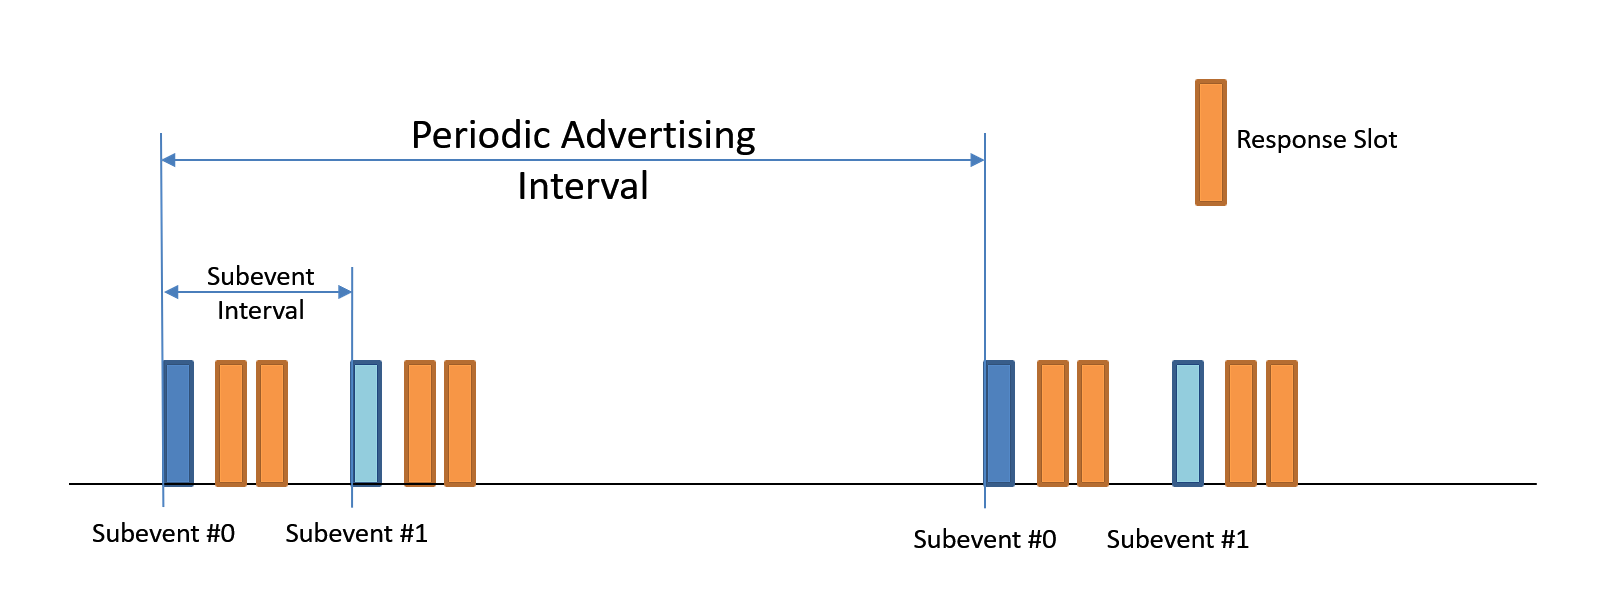
\includegraphics[width=0.85\linewidth]{./img/pawr_timing} 

}

\caption{PAwR 子事件与响应}\label{fig:ch-features-pawr}
\end{figure}

\hypertarget{ux5e7fux64adux6570ux636eux52a0ux5bc6}{%
\subsection{广播数据加密}\label{ux5e7fux64adux6570ux636eux52a0ux5bc6}}

旧版本的规范仅定义了连接模式下的加密,一直没有涉及广播数据的加密。这一新特性为加密广播数据提供了标准化方案。

广播数据的加密、鉴权沿用 CCM 算法,密钥信息通过新定义的 Encrypted Data Key Material 特征进行交换。
加密过的数据再打包到现有的 ``\protect\hyperlink{ch-overview-comm-model}{AD 结构}''里发送。

此特性可由 App 实现。

\hypertarget{ux5176ux5b83}{%
\section{其它}\label{ux5176ux5b83}}

\hypertarget{ux5e7fux64adux65f6-coded-phy-ux9009ux62e9}{%
\subsection{广播时 Coded PHY 选择}\label{ux5e7fux64adux65f6-coded-phy-ux9009ux62e9}}

当使用 Coded PHY 发送广播时,5.4 以前的 HCI 无法指定 S=2 或者 S=8。5.4 补上了这一``漏洞''。
SDK 一直支持\footnote{\url{https://github.com/ingchips/ING918XX_SDK_SOURCE/blob/75cbf9928711c39e0b234ae11796bc1696111998/bundles/typical/inc/platform_api.h\#L265}}
通过 API \texttt{ll\_set\_adv\_coded\_scheme} 选择 S=2 或者 S=8。

\hypertarget{ch-adv}{%
\chapter{GAP - 广播}\label{ch-adv}}

\hypertarget{ux6982ux89c8}{%
\section{概览}\label{ux6982ux89c8}}

支持 4.0 \textasciitilde{} 5.1 规范定义的所有 BLE 广播类型:

\begin{itemize}
\tightlist
\item
  传统广播(Legacy Adv)
\item
  扩展广播(Extended Adv)
\item
  周期广播(Periodic Adv)
\end{itemize}

传统广播的有效载荷最长为 \(31B\),而扩展广播(包括周期广播)每个广播包的有效载荷最长接近 \(255B\),
每个扩展广播又可包含多个广播包(广播包链条),总有效载荷最长达 \(1650B\)。

\hypertarget{ux7c7bux578b}{%
\subsection{类型}\label{ux7c7bux578b}}

广播有几种不同的属性:

\begin{itemize}
\item
  可连接:接受对方发来的连接建立请求
\item
  可扫描:接受对方发来的扫描请求,并回复扫描响应
\item
  定向:只用于可连接广播,只接受特定方发来的连接建立请求
\item
  高占空比(High Duty):以更高的频率\footnote{广播间隔小于 \(3.75ms\)。}重复发送广播数据,常用于实现快速重连(定向可连接广播),
  最长只持续 \(1.28s\)。从 5.0 开始,高占空比广播也可用于不可连接广播。
\end{itemize}

对于传统的扫描响应包,其有效载荷最长同样为 \(31B\);扩展的扫描响应包,其有效载荷最长同样为 \(1650B\)。
开发者可以要求协议栈收到扫描请求时上报事件。

总结起来,传统广播共有 5 种类型,见表 \ref{tab:ch1-legacy-adv-types}。

\begin{longtable}[]{@{}llll@{}}
\caption{\label{tab:ch1-legacy-adv-types} 传统广播类型}\tabularnewline
\toprule()
类型 & PDU 类型 & 广播数据 & 扫描响应数据 \\
\midrule()
\endfirsthead
\toprule()
类型 & PDU 类型 & 广播数据 & 扫描响应数据 \\
\midrule()
\endhead
非定向可连接可扫描广播 & ADV\_IND & 支持 & 支持 \\
定向可连接广播(非高占空比) & ADV\_DIRECT\_IND & 不支持 & 不支持 \\
定向可连接广播(高占空比) & ADV\_DIRECT\_IND & 不支持 & 不支持 \\
非定向可扫描广播 & ADV\_SCAN\_IND & 支持 & 支持 \\
非定向不可连接不可扫描广播 & ADV\_NONCONN\_IND & 支持 & 不支持 \\
\bottomrule()
\end{longtable}

\hypertarget{ch1-adv-filter}{%
\subsection{过滤策略}\label{ch1-adv-filter}}

对于可连接或可扫描广播,可以只接受某些设备的连接建立请求或扫描请求,这就是所谓的过滤策略。BLE 定义了 4 种策略:

\begin{Shaded}
\begin{Highlighting}[]
\KeywordTok{typedef} \KeywordTok{enum}\NormalTok{ adv\_filter\_policy}
\OperatorTok{\{}
    \CommentTok{// 接受所有的连接建立请求或扫描请求}
\NormalTok{    ADV\_FILTER\_ALLOW\_ALL    }\OperatorTok{=} \BaseNTok{0x00}\OperatorTok{,}
    \CommentTok{// 只接受白名单内的扫描请求,接收所有的连接建立请求}
\NormalTok{    ADV\_FILTER\_ALLOW\_SCAN\_WLST\_CON\_ALL}\OperatorTok{,}
    \CommentTok{// 只接受白名单内的连接建立请求,接收所有的扫描请求}
\NormalTok{    ADV\_FILTER\_ALLOW\_SCAN\_ALL\_CON\_WLST}\OperatorTok{,}
    \CommentTok{// 只接受白名单内的连接建立请求和扫描请求}
\NormalTok{    ADV\_FILTER\_ALLOW\_SCAN\_WLST\_CON\_WLST}
\OperatorTok{\}}\NormalTok{ adv\_filter\_policy\_t}\OperatorTok{;}
\end{Highlighting}
\end{Shaded}

\hypertarget{phy}{%
\subsection{PHY}\label{phy}}

对于扩展广播,既需要在主广播信道(37/38/39)上发送少量信息,也需要在其它信道(即辅广播信道)上发送,所以需要分别设置主、
辅广播信道所使用的 PHY,其中主广播信道只能使用 1M、Coded 等两种 PHY,而辅广播信道 3 种 PHY 皆可。

\hypertarget{ux5e7fux64adux96c6}{%
\subsection{广播集}\label{ux5e7fux64adux96c6}}

从 5.0 开始,BLE 支持并发发送多个广播,每个广播称为一个广播集\footnote{在不引起混淆的前提下,本手册混用``广播''、``广播集''这两个名词。},由广播集句柄指示。
每个广播使用各自独立的参数,包括地址、广播类型、PHY、数据等。
开发者可以为广播集指定一个 4 比特长的 SID。

\hypertarget{ux76f8ux5173ux4e8bux4ef6}{%
\subsection{相关事件}\label{ux76f8ux5173ux4e8bux4ef6}}

\begin{itemize}
\item
  \texttt{HCI\_SUBEVENT\_LE\_ADVERTISING\_SET\_TERMINATED}

  一个广播集停止广播时,HCI 回调会收到 \texttt{HCI\_SUBEVENT\_LE\_ADVERTISING\_SET\_TERMINATED} 事件。这个事件的触发条件如下:

  \begin{itemize}
  \tightlist
  \item
    连接建立:此时 \texttt{status} 为 \texttt{0},可读取广播句柄和连接句柄的对应关系;
  \item
    已达到预定的广播时长、次数,自动停止:此时 \texttt{status} 为 \texttt{0x43};
  \item
    极端情况:Controller 无法完成任务处理:此时 \texttt{status} 为 \texttt{0xFE}。
  \end{itemize}

  注意,高占空比广播停止时不上报此事件,而是上报 \texttt{HCI\_SUBEVENT\_LE\_ENHANCED\_CONNECTION\_COMPLETE} 事件。
  当未能建立连接高占空比广播超时时,\texttt{status} 置为 \texttt{0x3C}(定向广播超时)。
\item
  \texttt{HCI\_SUBEVENT\_LE\_SCAN\_REQUEST\_RECEIVED}

  开发者使能扫描请求指示后,HCI 回调会收到 \texttt{HCI\_SUBEVENT\_LE\_SCAN\_REQUEST\_RECEIVED} 事件。
\item
  \texttt{HCI\_SUBEVENT\_PRD\_ADV\_SUBEVT\_DATA\_REQ}

  发送 PAwR 时,通过该事件向上层应用请求设置子事件数据。该事件的内容为
  \texttt{le\_mete\_event\_prd\_adv\_subevent\_data\_req\_t}。应用收到该事件后,可通过
  \texttt{gap\_set\_periodic\_adv\_subevent\_data} 为子事件设置数据。
\item
  \texttt{HCI\_SUBEVENT\_PRD\_ADV\_RSP\_REPORT}

  收到 PAwR 的响应时,HCI 回调会收到 \texttt{HCI\_SUBEVENT\_PRD\_ADV\_RSP\_REPORT} 事件,其内容为
  \texttt{le\_mete\_event\_prd\_adv\_rsp\_report\_t}。
\end{itemize}

\hypertarget{ux4f7fux7528ux8bf4ux660e}{%
\section{使用说明}\label{ux4f7fux7528ux8bf4ux660e}}

\hypertarget{ux914dux7f6eux5e7fux64ad}{%
\subsection{配置广播}\label{ux914dux7f6eux5e7fux64ad}}

主要用到 4 个函数,\texttt{gap\_set\_adv\_set\_random\_addr}、\texttt{gap\_set\_ext\_adv\_para}、\texttt{gap\_set\_ext\_adv\_data} 和 \texttt{gap\_set\_ext\_scan\_response\_data},
分别配置随机地址、参数、广播数据和扫描响应数据。
参数最复杂的函数是 \texttt{gap\_set\_ext\_adv\_para},其原型为:

\begin{Shaded}
\begin{Highlighting}[]
\DataTypeTok{uint8\_t}\NormalTok{ gap\_set\_ext\_adv\_para}\OperatorTok{(}
    \CommentTok{// 广播集句柄}
    \DataTypeTok{const} \DataTypeTok{uint8\_t}\NormalTok{ adv\_handle}\OperatorTok{,}
    \CommentTok{// 属性比特组合}
    \DataTypeTok{const}\NormalTok{ adv\_event\_properties\_t properties}\OperatorTok{,}
    \CommentTok{// 广播间隔}
    \DataTypeTok{const} \DataTypeTok{uint32\_t}\NormalTok{ interval\_min}\OperatorTok{,}
    \DataTypeTok{const} \DataTypeTok{uint32\_t}\NormalTok{ interval\_max}\OperatorTok{,}
    \CommentTok{// 使用的主广播信道比特组合(0x7 表示使用全部 3 个主广播信道)}
    \DataTypeTok{const}\NormalTok{ adv\_channel\_bits\_t primary\_adv\_channel\_map}\OperatorTok{,}
    \CommentTok{// 使用的地址类型(随机地址来自 gap\_set\_adv\_set\_random\_addr)}
    \DataTypeTok{const}\NormalTok{ bd\_addr\_type\_t own\_addr\_type}\OperatorTok{,}
    \CommentTok{// 设置定向广播的对端地址}
    \DataTypeTok{const}\NormalTok{ bd\_addr\_type\_t peer\_addr\_type}\OperatorTok{,}
    \DataTypeTok{const} \DataTypeTok{uint8\_t} \OperatorTok{*}\NormalTok{peer\_addr}\OperatorTok{,}
    \CommentTok{// 过滤策略}
    \DataTypeTok{const}\NormalTok{ adv\_filter\_policy\_t adv\_filter\_policy}\OperatorTok{,}
    \CommentTok{// 发射功率,单位为 dBm}
    \DataTypeTok{const} \DataTypeTok{int8\_t}\NormalTok{ tx\_power}\OperatorTok{,}
    \CommentTok{// 主信道 PHY}
    \DataTypeTok{const}\NormalTok{ phy\_type\_t primary\_adv\_phy}\OperatorTok{,}
    \CommentTok{// 是否允许跳过部分辅信道的发送(填 0 表示总是发送)}
    \DataTypeTok{const} \DataTypeTok{uint8\_t}\NormalTok{ secondary\_adv\_max\_skip}\OperatorTok{,}
    \CommentTok{// 辅信道 PHY}
    \DataTypeTok{const}\NormalTok{ phy\_type\_t secondary\_adv\_phy}\OperatorTok{,}
    \CommentTok{// 广播集 SID}
    \DataTypeTok{const} \DataTypeTok{uint8\_t}\NormalTok{ sid}\OperatorTok{,}
    \CommentTok{// 使能扫描请求上报}
    \DataTypeTok{const} \DataTypeTok{uint8\_t}\NormalTok{ scan\_req\_notification\_enable}\OperatorTok{);}
\end{Highlighting}
\end{Shaded}

其中,\texttt{properties} 为以下比特的组合:

\begin{Shaded}
\begin{Highlighting}[]
\CommentTok{// 可连接广播}
\PreprocessorTok{\#define    CONNECTABLE\_ADV\_BIT       ...}
\CommentTok{// 可扫描广播}
\PreprocessorTok{\#define    SCANNABLE\_ADV\_BIT         ...}
\CommentTok{// 定向广播}
\PreprocessorTok{\#define    DIRECT\_ADV\_BIT            ...}
\CommentTok{// 高频广播}
\PreprocessorTok{\#define    HIGH\_DUTY\_CIR\_DIR\_ADV\_BIT ...}
\CommentTok{// 传统广播}
\PreprocessorTok{\#define    LEGACY\_PDU\_BIT            ...}
\CommentTok{// 匿名广播}
\PreprocessorTok{\#define    ANONY\_ADV\_BIT             ...}
\CommentTok{// 包含发射功率}
\PreprocessorTok{\#define    INC\_TX\_ADV\_BIT            ...}
\end{Highlighting}
\end{Shaded}

对于传统广播,比特组合必须符合表 \ref{tab:ch1-legacy-adv-types} 的定义。
对于扩展广播,不能既可连接又可扫描;不支持高占空比广播。
匿名广播中不包含广播者的地址,所以称为``匿名''广播。附加 \texttt{INC\_TX\_ADV\_BIT} 比特后,
广播内自动包含发射功率,比在载荷内通过 AD 项 ``0x0A - «Tx Power Level»''发送开销更小。

\hypertarget{ch1-adv-data-edit}{%
\subsection{广播数据}\label{ch1-adv-data-edit}}

使用 Wizard 里的广播数据编辑器可以方便地编辑数据\footnote{请参阅 SDK 用户手册。}。
广播数据编辑器同时可以生成一些常数,方便开发者编程修改广播数据。
下面的例子把蓝牙地址的最末两个字节填充到设备名称的最后 4 个字符里。

\begin{enumerate}
\def\labelenumi{\arabic{enumi}.}
\item
  用广播数据编辑器生成初始数据(图 \ref{fig:ch0-gen-adv-data}):

  \begin{figure}

   {\centering 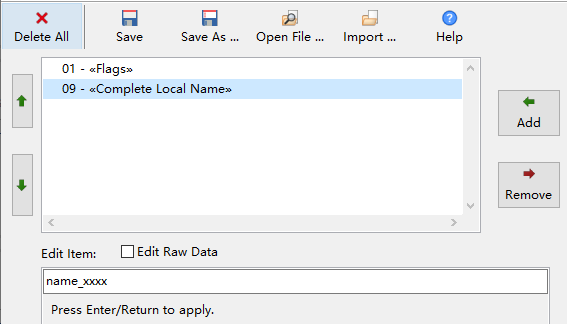
\includegraphics[width=0.6\linewidth]{./img/gen_adv_data} 

   }

   \caption{用广播数据编辑器生成初始数据}\label{fig:ch0-gen-adv-data}
   \end{figure}

\begin{Shaded}
\begin{Highlighting}[]
\CommentTok{// 0x01 {-} «Flags»}
\DecValTok{2}\OperatorTok{,} \BaseNTok{0x01}\OperatorTok{,}
\BaseNTok{0x06}\OperatorTok{,}

\CommentTok{// 0x09 {-} «Complete Local Name»: name\_xxxx}
\DecValTok{10}\OperatorTok{,} \BaseNTok{0x09}\OperatorTok{,}
\BaseNTok{0x6E}\OperatorTok{,} \BaseNTok{0x61}\OperatorTok{,} \BaseNTok{0x6D}\OperatorTok{,} \BaseNTok{0x65}\OperatorTok{,} \BaseNTok{0x5F}\OperatorTok{,} \BaseNTok{0x78}\OperatorTok{,} \BaseNTok{0x78}\OperatorTok{,} \BaseNTok{0x78}\OperatorTok{,}
\BaseNTok{0x78}\OperatorTok{,}

\CommentTok{// Total size = 14 bytes}
\end{Highlighting}
\end{Shaded}
\item
  导入广播数据及常数:

\begin{Shaded}
\begin{Highlighting}[]
\DataTypeTok{static} \DataTypeTok{uint8\_t}\NormalTok{ adv\_data}\OperatorTok{[]} \OperatorTok{=} \OperatorTok{\{}
    \PreprocessorTok{\#include }\ImportTok{"../data/advertising.adv"}
\OperatorTok{\};}
\CommentTok{// 这个文件里是编辑器生成的常数}
\PreprocessorTok{\#include }\ImportTok{"../data/advertising.const"}
\end{Highlighting}
\end{Shaded}
\item
  修改广播名称

\begin{Shaded}
\begin{Highlighting}[]
\DataTypeTok{void}\NormalTok{ assign\_name}\OperatorTok{(}\DataTypeTok{const} \DataTypeTok{uint8\_t} \OperatorTok{*}\NormalTok{id\_bytes}\OperatorTok{)}
\OperatorTok{\{}
    \DataTypeTok{char}\NormalTok{ temp}\OperatorTok{[}\DecValTok{5}\OperatorTok{];}
\NormalTok{    sprintf}\OperatorTok{(}\NormalTok{temp}\OperatorTok{,} \StringTok{"\%02X\%02X"}\OperatorTok{,}\NormalTok{ id\_bytes}\OperatorTok{[}\DecValTok{0}\OperatorTok{],}\NormalTok{ id\_bytes}\OperatorTok{[}\DecValTok{1}\OperatorTok{]);}
    \CommentTok{// ADVERTISING\_ITEM\_OFFSET\_COMPLETE\_LOCAL\_NAME 是编译器自动生成的常数,}
    \CommentTok{// 表示 "name\_xxxx" 在整个数据里的偏移位置}
\NormalTok{    memcpy}\OperatorTok{(}\NormalTok{adv\_data }\OperatorTok{+}\NormalTok{ ADVERTISING\_ITEM\_OFFSET\_COMPLETE\_LOCAL\_NAME }\OperatorTok{+} \DecValTok{5}\OperatorTok{,}
\NormalTok{           temp}\OperatorTok{,} \KeywordTok{sizeof}\OperatorTok{(}\NormalTok{temp}\OperatorTok{)} \OperatorTok{{-}} \DecValTok{1}\OperatorTok{);}
\OperatorTok{\}}
\CommentTok{// 假设地址存放于 rand\_addr}
\NormalTok{assign\_name}\OperatorTok{(\&}\NormalTok{rand\_addr}\OperatorTok{[}\DecValTok{4}\OperatorTok{]);}
\end{Highlighting}
\end{Shaded}
\end{enumerate}

\hypertarget{ux914dux7f6eux5468ux671fux5e7fux64ad}{%
\subsection{配置周期广播}\label{ux914dux7f6eux5468ux671fux5e7fux64ad}}

周期广播总是与一个不可连接、不可扫描的扩展广播绑定。使用 \texttt{gap\_set\_ext\_adv\_para} 设置了扩展广播参数后,
就可以通过 \texttt{gap\_set\_periodic\_adv\_para} 创建相关联的周期广播:

\begin{Shaded}
\begin{Highlighting}[]
\DataTypeTok{uint8\_t}\NormalTok{ gap\_set\_periodic\_adv\_para}\OperatorTok{(}
  \CommentTok{// 使用同一个广播集句柄}
  \DataTypeTok{const} \DataTypeTok{uint8\_t}\NormalTok{ adv\_handle}\OperatorTok{,}
  \CommentTok{// 广播周期}
  \DataTypeTok{const} \DataTypeTok{uint16\_t}\NormalTok{ interval\_min}\OperatorTok{,}
  \DataTypeTok{const} \DataTypeTok{uint16\_t}\NormalTok{ interval\_max}\OperatorTok{,}
  \CommentTok{// 属性(仅支持 0 或 PERIODIC\_ADV\_BIT\_INC\_TX)}
  \DataTypeTok{const}\NormalTok{ periodic\_adv\_properties\_t properties}\OperatorTok{);}
\end{Highlighting}
\end{Shaded}

周期广播的数据通过 \texttt{gap\_set\_periodic\_adv\_data} 设置,而不是 \texttt{gap\_set\_ext\_adv\_para}。

\hypertarget{ux8d77ux505cux5e7fux64ad}{%
\subsection{起停广播}\label{ux8d77ux505cux5e7fux64ad}}

通过 \texttt{gap\_set\_ext\_adv\_enable} 控制多个广播集的使能、停止状态。

\begin{Shaded}
\begin{Highlighting}[]
\DataTypeTok{uint8\_t}\NormalTok{ gap\_set\_ext\_adv\_enable}\OperatorTok{(}
  \CommentTok{// 使能还是停止?}
  \DataTypeTok{const} \DataTypeTok{uint8\_t}\NormalTok{ enable}\OperatorTok{,}
  \CommentTok{// 广播集数目}
  \DataTypeTok{const} \DataTypeTok{uint8\_t}\NormalTok{ set\_number}\OperatorTok{,}
  \CommentTok{// 每个广播集的使能参数}
  \DataTypeTok{const}\NormalTok{ ext\_adv\_set\_en\_t }\OperatorTok{*}\NormalTok{adv\_sets}\OperatorTok{);}
\end{Highlighting}
\end{Shaded}

这个函数支持一种快速停止所有广播的用法:\texttt{gap\_set\_ext\_adv\_enable(0,\ 0,\ NULL)}。除此以外,都需要用 \texttt{adv\_sets}
数组表明每个广播集的句柄。

对于使能广播的情况,\texttt{adv\_sets} 使用另外两个参数用来控制广播次数:

\begin{Shaded}
\begin{Highlighting}[]
\KeywordTok{typedef} \KeywordTok{struct}\NormalTok{ ext\_adv\_set\_en}
\OperatorTok{\{}
    \DataTypeTok{uint8\_t}\NormalTok{ handle}\OperatorTok{;}
    \CommentTok{// 广播持续时间,单位为 10ms。0ms 表示一直广播}
    \DataTypeTok{uint16\_t}\NormalTok{ duration}\OperatorTok{;}
    \CommentTok{// 最大广播次数。0 表示一直广播}
    \DataTypeTok{uint8\_t}\NormalTok{ max\_events}\OperatorTok{;}
\OperatorTok{\}}\NormalTok{ ext\_adv\_set\_en\_t}\OperatorTok{;}
\end{Highlighting}
\end{Shaded}

当 \texttt{duration} 或 \texttt{max\_events} 条件满足时,广播就会自动停止。

\hypertarget{ux8d77ux505cux5468ux671fux5e7fux64ad}{%
\subsection{起停周期广播}\label{ux8d77ux505cux5468ux671fux5e7fux64ad}}

周期广播需要使用 \texttt{gap\_set\_periodic\_adv\_enable} 控制使能、停止状态:

\begin{Shaded}
\begin{Highlighting}[]
\DataTypeTok{uint8\_t}\NormalTok{ gap\_set\_periodic\_adv\_enable}\OperatorTok{(}
  \DataTypeTok{const} \DataTypeTok{uint8\_t}\NormalTok{ enable}\OperatorTok{,}
  \DataTypeTok{const} \DataTypeTok{uint8\_t}\NormalTok{ adv\_handle}\OperatorTok{);}
\end{Highlighting}
\end{Shaded}

要``完整''地开启周期广播,需要先通过 \texttt{gap\_set\_ext\_adv\_enable} 使能关联的扩展广播,再用这个 API 使能周期广播。
扩展广播可以独立地关闭\footnote{关闭之后,其它设备无法再与该周期广播建立同步。}。

\hypertarget{ux4e3aux5468ux671fux5e7fux64adux6dfbux52a0-cte}{%
\subsection{为周期广播添加 CTE}\label{ux4e3aux5468ux671fux5e7fux64adux6dfbux52a0-cte}}

参考``\protect\hyperlink{misc-cte-periodic-adv}{基于周期广播的 CTE 接收和发送}''一节。

\hypertarget{ux5e26ux54cdux5e94ux7684ux5468ux671fux5e7fux64adpawr-1}{%
\subsection{带响应的周期广播(PAwR)}\label{ux5e26ux54cdux5e94ux7684ux5468ux671fux5e7fux64adpawr-1}}

\hypertarget{ux914dux7f6e}{%
\subsubsection{配置}\label{ux914dux7f6e}}

PAwR 广播也总是与一个不可连接、不可扫描的扩展广播绑定。使用 \texttt{gap\_set\_ext\_adv\_para} 设置了扩展广播参数后,
就可以通过 \texttt{gap\_set\_periodic\_adv\_para\_v2} 创建相关联的 PAwR 广播,与 \texttt{gap\_set\_periodic\_adv\_para}
相比,增加了几个关于 PAwR 的参数:

\begin{Shaded}
\begin{Highlighting}[]
\DataTypeTok{uint8\_t}\NormalTok{ gap\_set\_periodic\_adv\_para\_v2}\OperatorTok{(}
  \CommentTok{// 使用同一个广播集句柄}
  \DataTypeTok{const} \DataTypeTok{uint8\_t}\NormalTok{ adv\_handle}\OperatorTok{,}
  \CommentTok{// 广播周期}
  \DataTypeTok{const} \DataTypeTok{uint16\_t}\NormalTok{ interval\_min}\OperatorTok{,}
  \DataTypeTok{const} \DataTypeTok{uint16\_t}\NormalTok{ interval\_max}\OperatorTok{,}
  \CommentTok{// 属性(仅支持 0 或 PERIODIC\_ADV\_BIT\_INC\_TX)}
  \DataTypeTok{const}\NormalTok{ periodic\_adv\_properties\_t properties}\OperatorTok{,}
  \CommentTok{// 子事件个数}
  \DataTypeTok{const} \DataTypeTok{uint8\_t}\NormalTok{ num\_subevents}\OperatorTok{,}
  \CommentTok{// 子事件间隔}
  \DataTypeTok{const} \DataTypeTok{uint8\_t}\NormalTok{ subevent\_interval}\OperatorTok{,}
  \CommentTok{// 第一个响应时隙的延迟}
  \DataTypeTok{const} \DataTypeTok{uint8\_t}\NormalTok{ response\_slot\_delay}\OperatorTok{,}
  \CommentTok{// 响应时隙的间隔}
  \DataTypeTok{const} \DataTypeTok{uint8\_t}\NormalTok{ response\_slot\_spacing}\OperatorTok{,}
  \CommentTok{// 每个子事件的响应时隙数}
  \DataTypeTok{const} \DataTypeTok{uint8\_t}\NormalTok{ num\_response\_slots}\OperatorTok{);}
\end{Highlighting}
\end{Shaded}

\hypertarget{ux4e3aux5b50ux4e8bux4ef6ux8bbeux7f6eux66f4ux65b0ux6570ux636e}{%
\subsubsection{为子事件设置、更新数据}\label{ux4e3aux5b50ux4e8bux4ef6ux8bbeux7f6eux66f4ux65b0ux6570ux636e}}

当收到 \texttt{HCI\_SUBEVENT\_PRD\_ADV\_SUBEVT\_DATA\_REQ} 事件时,通过
\texttt{gap\_set\_periodic\_adv\_subevent\_data} 为子事件设置数据:

\begin{Shaded}
\begin{Highlighting}[]
\DataTypeTok{uint8\_t}\NormalTok{ gap\_set\_periodic\_adv\_subevent\_data}\OperatorTok{(}
  \CommentTok{// PAwR 的广播集句柄}
  \DataTypeTok{uint8\_t}\NormalTok{ adv\_handle}\OperatorTok{,}
  \CommentTok{// 要设置的子事件的个数}
  \DataTypeTok{uint8\_t}\NormalTok{ num\_subevents}\OperatorTok{,}
  \CommentTok{// 每个子事件的数据}
  \DataTypeTok{const}\NormalTok{ gap\_prd\_adv\_subevent\_data\_t }\OperatorTok{*}\NormalTok{data}\OperatorTok{);}
\end{Highlighting}
\end{Shaded}

每个子事件的数据定义如下:

\begin{Shaded}
\begin{Highlighting}[]
\KeywordTok{typedef} \KeywordTok{struct}
\OperatorTok{\{}
    \CommentTok{// 子事件序号}
    \DataTypeTok{uint8\_t}\NormalTok{         subevent}\OperatorTok{;}
    \CommentTok{// 本子事件的第一个响应时隙的序号}
    \DataTypeTok{uint8\_t}\NormalTok{         rsp\_slot\_start}\OperatorTok{;}
    \CommentTok{// 本子事件的响应时隙的个数}
    \DataTypeTok{uint8\_t}\NormalTok{         rsp\_slot\_count}\OperatorTok{;}
    \CommentTok{// 数据长度}
    \DataTypeTok{uint8\_t}\NormalTok{         data\_len}\OperatorTok{;}
    \CommentTok{// 数据}
    \DataTypeTok{const} \DataTypeTok{uint8\_t} \OperatorTok{*}\NormalTok{ data}\OperatorTok{;}
\OperatorTok{\}}\NormalTok{ gap\_prd\_adv\_subevent\_data\_t}\OperatorTok{;}
\end{Highlighting}
\end{Shaded}

这里设置的响应时隙应为 \texttt{gap\_set\_periodic\_adv\_para\_v2} 所设置的响应时隙的子集。

\hypertarget{ch-adv-create-connection}{%
\subsubsection{从 PAwR 发起连接}\label{ch-adv-create-connection}}

通过 \texttt{gap\_ext\_create\_connection\_v2} 在指定的子事件上向指定设备发送连接请求。
\texttt{gap\_ext\_create\_connection\_v2} 是 \protect\hyperlink{ch-scan-create-connection}{\texttt{gap\_ext\_create\_connection}}
的增强版本,增加了 2 个参数:
\texttt{adv\_handle} 和 \texttt{subevent}。当这两个参数都是无效值(0xff)时,\texttt{gap\_ext\_create\_connection\_v2}
的功能等同于 \texttt{gap\_ext\_create\_connection}。从 PAwR 发起连接时,这两个参数应该为有效值,此时, 忽略
\texttt{filter\_policy},以及 \texttt{phy\_configs} 里的 \texttt{phy}、\texttt{scan\_int}、\texttt{scan\_win}。

\begin{Shaded}
\begin{Highlighting}[]
\DataTypeTok{uint8\_t}\NormalTok{ gap\_ext\_create\_connection\_v2}\OperatorTok{(}
  \CommentTok{// PAwR 的广播集句柄}
  \DataTypeTok{const} \DataTypeTok{uint8\_t}\NormalTok{ adv\_handle}\OperatorTok{,}
  \CommentTok{// 子事件序号}
  \DataTypeTok{const} \DataTypeTok{uint8\_t}\NormalTok{ subevent}\OperatorTok{,}
  \DataTypeTok{const}\NormalTok{ initiating\_filter\_policy\_t filter\_policy}\OperatorTok{,}
  \DataTypeTok{const}\NormalTok{ bd\_addr\_type\_t own\_addr\_type}\OperatorTok{,}
  \DataTypeTok{const}\NormalTok{ bd\_addr\_type\_t peer\_addr\_type}\OperatorTok{,}
  \DataTypeTok{const} \DataTypeTok{uint8\_t} \OperatorTok{*}\NormalTok{peer\_addr}\OperatorTok{,}
  \DataTypeTok{const} \DataTypeTok{uint8\_t}\NormalTok{ initiating\_phy\_num}\OperatorTok{,}
  \DataTypeTok{const}\NormalTok{ initiating\_phy\_config\_t }\OperatorTok{*}\NormalTok{phy\_configs}
  \OperatorTok{);}
\end{Highlighting}
\end{Shaded}

\hypertarget{ch-scan}{%
\chapter{GAP - 扫描}\label{ch-scan}}

\hypertarget{ux6982ux89c8-1}{%
\section{概览}\label{ux6982ux89c8-1}}

接收广播的过程称为扫描。

\hypertarget{ux95f4ux9694ux4e0eux7a97ux53e3}{%
\subsection{间隔与窗口}\label{ux95f4ux9694ux4e0eux7a97ux53e3}}

接收机实际进行扫描工作的时机受扫描间隔和窗口两个参数控制,其含义如图 \ref{fig:ch2-scan-win-interval} 所示。

\begin{figure}

{\centering 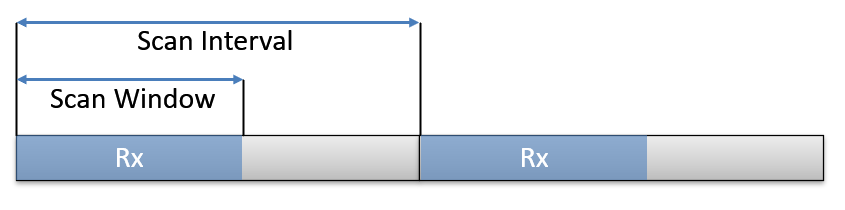
\includegraphics[width=0.7\linewidth]{./img/scan_win_interval} 

}

\caption{扫描间隔与扫描窗口}\label{fig:ch2-scan-win-interval}
\end{figure}

\textbf{注意}:Controller 在执行扫描任务时,遵循最大努力原则,实际真正用于扫描的时机可能并不与两个参数所指定的完全一致。

\hypertarget{ux8fc7ux6ee4ux7b56ux7565}{%
\subsection{过滤策略}\label{ux8fc7ux6ee4ux7b56ux7565}}

与广播的``\protect\hyperlink{ch1-adv-filter}{过滤策略}''类似,扫描也有几种过滤策略:

\begin{Shaded}
\begin{Highlighting}[]
\KeywordTok{typedef} \KeywordTok{enum}\NormalTok{ scan\_filter\_policy}
\OperatorTok{\{}
    \CommentTok{// 接收所有广播(定向到其它设备的除外)}
\NormalTok{    SCAN\_ACCEPT\_ALL\_EXCEPT\_NOT\_DIRECTED}\OperatorTok{,}
    \CommentTok{// 只接收来自白名单内的设备的广播(定向到其它设备的除外)}
\NormalTok{    SCAN\_ACCEPT\_WLIST\_EXCEPT\_NOT\_DIRECTED}\OperatorTok{,}
    \CommentTok{// 接收所有广播(所定向的设备与本设备身份地址不同的除外)}
\NormalTok{    SCAN\_ACCEPT\_ALL\_EXCEPT\_IDENTITY\_NOT\_MATCH}\OperatorTok{,}
    \CommentTok{// 只接收来自白名单内的设备的广播(所定向的设备与本设备身份地址不同的除外)}
\NormalTok{    SCAN\_ACCEPT\_WLIST\_EXCEPT\_IDENTITY\_NOT\_MATCH}
\OperatorTok{\}}\NormalTok{ scan\_filter\_policy\_t}\OperatorTok{;}
\end{Highlighting}
\end{Shaded}

\hypertarget{ux4e3bux52a8ux4e0eux88abux52a8}{%
\subsection{主动与被动}\label{ux4e3bux52a8ux4e0eux88abux52a8}}

所谓被动扫描(Passive Scan)指只接收广播数据包,对于可扫描广播也是如此;所谓主动扫描(Active Scan)指除了接收广播数据包之外,
对于可扫描广播会主动发送扫描请求并接收扫描响应包。

\hypertarget{phy-1}{%
\subsection{PHY}\label{phy-1}}

由于扩展广播可在主广播信道使用两种 PHY 发送,相应地,扫描时也需要配置扫描哪种 PHY。

\hypertarget{ux4f7fux7528ux8bf4ux660e-1}{%
\section{使用说明}\label{ux4f7fux7528ux8bf4ux660e-1}}

\hypertarget{ux914dux7f6eux53c2ux6570}{%
\subsection{配置参数}\label{ux914dux7f6eux53c2ux6570}}

在开始扫描之前,需要先通过 \texttt{gap\_set\_random\_device\_address} 为设备配置地址,这个地址用于扫描、发起连接等场景。
使用 \texttt{gap\_set\_ext\_scan\_para} 配置扫描参数:

\begin{Shaded}
\begin{Highlighting}[]
\DataTypeTok{uint8\_t}\NormalTok{ gap\_set\_ext\_scan\_para}\OperatorTok{(}
  \CommentTok{// 本设备地址类型}
  \DataTypeTok{const}\NormalTok{ bd\_addr\_type\_t own\_addr\_type}\OperatorTok{,}
  \CommentTok{// 过滤策略}
  \DataTypeTok{const}\NormalTok{ scan\_filter\_policy\_t filter}\OperatorTok{,}
  \CommentTok{// PHY 配置个数}
  \DataTypeTok{const} \DataTypeTok{uint8\_t}\NormalTok{ config\_num}\OperatorTok{,}
  \CommentTok{// 关于每种 PHY 的参数配置}
  \DataTypeTok{const}\NormalTok{ scan\_phy\_config\_t }\OperatorTok{*}\NormalTok{configs}\OperatorTok{);}
\end{Highlighting}
\end{Shaded}

这里的 PHY 指的是主广播信道所使用的 PHY,只能为 1M 或 Coded。辅广播信道上所有的 PHY 类型全部支持,不需要配置。
每种 PHY 的参数配置如下:

\begin{Shaded}
\begin{Highlighting}[]
\KeywordTok{typedef} \KeywordTok{struct}\NormalTok{ scan\_phy\_config}
\OperatorTok{\{}
    \CommentTok{// PHY}
\NormalTok{    phy\_type\_t phy}\OperatorTok{;}
    \CommentTok{// 扫描方式:主动或被动}
\NormalTok{    scan\_type\_t type}\OperatorTok{;}
    \CommentTok{// 扫描间隔,单位是 625us}
    \DataTypeTok{uint16\_t}\NormalTok{ interval}\OperatorTok{;}
    \CommentTok{// 扫描窗口,单位是 625us}
    \DataTypeTok{uint16\_t}\NormalTok{ window}\OperatorTok{;}
\OperatorTok{\}}\NormalTok{ scan\_phy\_config\_t}\OperatorTok{;}
\end{Highlighting}
\end{Shaded}

\hypertarget{ux8d77ux505cux626bux63cf}{%
\subsection{起停扫描}\label{ux8d77ux505cux626bux63cf}}

使用 \texttt{gap\_set\_ext\_scan\_enable} 起停扫描:

\begin{Shaded}
\begin{Highlighting}[]
\DataTypeTok{uint8\_t}\NormalTok{ gap\_set\_ext\_scan\_enable}\OperatorTok{(}
  \CommentTok{// 开始或者停止扫描}
  \DataTypeTok{const} \DataTypeTok{uint8\_t}\NormalTok{ enable}\OperatorTok{,}
  \CommentTok{// 是否对数据做去重处理:}
  \CommentTok{// 0 {-} 不去重;}
  \CommentTok{// 1 {-} 去重;}
  \CommentTok{// 2 {-} 去重,但是每个周期复位过滤器}
  \DataTypeTok{const} \DataTypeTok{uint8\_t}\NormalTok{ filter}\OperatorTok{,}
  \CommentTok{// 持续时间,单位为 10ms}
  \DataTypeTok{const} \DataTypeTok{uint16\_t}\NormalTok{ duration}\OperatorTok{,}
  \CommentTok{// 周期,单位为 1.28s}
  \DataTypeTok{const} \DataTypeTok{uint16\_t}\NormalTok{ period}\OperatorTok{);}
\end{Highlighting}
\end{Shaded}

\texttt{duration} 和 \texttt{period} 两个参数的目的是实现每个 \texttt{period} 里扫描 \texttt{duration} 长的时间。另有两种特殊情况,从开发者的角度总结如下:

\begin{enumerate}
\def\labelenumi{\arabic{enumi}.}
\tightlist
\item
  持续、一直地扫描:\texttt{duration} 和 \texttt{period} 两个参数皆置为 \(0\)
\item
  只扫描一段时间:\texttt{duration} 置为扫描时长,\texttt{period} 置为 \(0\)
\end{enumerate}

\begin{rmdcaution}
Controller
在做数据去重时遵循最大努力原则,受限于存储空间、处理能力,去重可能失效。
\end{rmdcaution}

\hypertarget{ux5904ux7406ux6570ux636e}{%
\subsection{处理数据}\label{ux5904ux7406ux6570ux636e}}

收到广播包后,HCI 回调函数将收到 \texttt{HCI\_SUBEVENT\_LE\_EXTENDED\_ADVERTISING\_REPORT} 事件。利用 \texttt{decode\_hci\_le\_meta\_event}
宏可将事件转换为 \texttt{le\_ext\_adv\_report\_t} 结构体指针:

\begin{Shaded}
\begin{Highlighting}[]
\DataTypeTok{const}\NormalTok{ le\_ext\_adv\_report\_t }\OperatorTok{*}\NormalTok{report }\OperatorTok{=}
\NormalTok{  decode\_hci\_le\_meta\_event}\OperatorTok{(}\NormalTok{packet}\OperatorTok{,}\NormalTok{ le\_meta\_event\_ext\_adv\_report\_t}\OperatorTok{){-}\textgreater{}}\NormalTok{reports}\OperatorTok{;}
\end{Highlighting}
\end{Shaded}

这个结构体的定义如下:

\begin{Shaded}
\begin{Highlighting}[]
\KeywordTok{typedef} \KeywordTok{struct}\NormalTok{ le\_ext\_adv\_report}
\OperatorTok{\{}
    \CommentTok{// 事件类型比特位组合}
    \DataTypeTok{uint16\_t}\NormalTok{        evt\_type}\OperatorTok{;}
    \CommentTok{// 广播者地址类型}
\NormalTok{    bd\_addr\_type\_t  addr\_type}\OperatorTok{;}
    \CommentTok{// 广播者地址}
\NormalTok{    bd\_addr\_t       address}\OperatorTok{;}
    \CommentTok{// 主信道上用的 PHY}
    \DataTypeTok{uint8\_t}\NormalTok{         p\_phy}\OperatorTok{;}
    \CommentTok{// 辅信道上用的 PHY}
    \DataTypeTok{uint8\_t}\NormalTok{         s\_phy}\OperatorTok{;}
    \CommentTok{// SID}
    \DataTypeTok{uint8\_t}\NormalTok{         sid}\OperatorTok{;}
    \CommentTok{// 发射功率(单位 dBm)}
     \DataTypeTok{int8\_t}\NormalTok{         tx\_power}\OperatorTok{;}
    \CommentTok{// RSSI (单位 dBm)}
     \DataTypeTok{int8\_t}\NormalTok{         rssi}\OperatorTok{;}
    \CommentTok{// 周期广播的间隔(仅对周期广播有效)}
    \DataTypeTok{uint16\_t}\NormalTok{        prd\_adv\_interval}\OperatorTok{;}
    \CommentTok{// 定向广播的目的地址类型}
\NormalTok{    bd\_addr\_type\_t  direct\_addr\_type}\OperatorTok{;}
    \CommentTok{// 定向广播的目的地址}
\NormalTok{    bd\_addr\_t       direct\_addr}\OperatorTok{;}
    \CommentTok{// 广播数据长度}
    \DataTypeTok{uint8\_t}\NormalTok{         data\_len}\OperatorTok{;}
    \CommentTok{// 广播数据}
    \DataTypeTok{uint8\_t}\NormalTok{         data}\OperatorTok{[}\DecValTok{0}\OperatorTok{];}
\OperatorTok{\}}\NormalTok{ le\_ext\_adv\_report\_t}\OperatorTok{;}
\end{Highlighting}
\end{Shaded}

\hypertarget{ux4e0eux5468ux671fux5e7fux64adux540cux6b65}{%
\subsection{与周期广播同步}\label{ux4e0eux5468ux671fux5e7fux64adux540cux6b65}}

发现周期广播后,可以通过 \texttt{gap\_periodic\_adv\_create\_sync} 与周期广播同步\footnote{即周期性地接收周期广播。}:

\begin{Shaded}
\begin{Highlighting}[]
\DataTypeTok{uint8\_t}\NormalTok{ gap\_periodic\_adv\_create\_sync}\OperatorTok{(}
  \CommentTok{// 过滤策略:目标地址来自白名单还是参数}
  \DataTypeTok{const}\NormalTok{ periodic\_adv\_filter\_policy\_t filter\_policy}\OperatorTok{,}
  \CommentTok{// SID}
  \DataTypeTok{const} \DataTypeTok{uint8\_t}\NormalTok{ adv\_sid}\OperatorTok{,}
  \CommentTok{// 目标地址类型}
  \DataTypeTok{const}\NormalTok{ bd\_addr\_type\_t addr\_type}\OperatorTok{,}
  \CommentTok{// 目标地址}
  \DataTypeTok{const} \DataTypeTok{uint8\_t} \OperatorTok{*}\NormalTok{addr}\OperatorTok{,}
  \CommentTok{// 成功接收一次之后,可跳过的数目}
  \DataTypeTok{const} \DataTypeTok{uint16\_t}\NormalTok{ skip}\OperatorTok{,}
  \CommentTok{// 同步超时(单位 100ms)}
  \DataTypeTok{const} \DataTypeTok{uint16\_t}\NormalTok{ sync\_timeout}\OperatorTok{,}
  \CommentTok{// 周期广播里的 CTE 类型(如果存在)}
  \DataTypeTok{const} \DataTypeTok{uint8\_t}\NormalTok{ sync\_cte\_type}
\OperatorTok{);}
\end{Highlighting}
\end{Shaded}

成功建立同步后,HCI 回调会收到 \texttt{HCI\_SUBEVENT\_LE\_PERIODIC\_ADVERTISING\_SYNC\_ESTABLISHED} 事件。接收到的周期广播通过
\texttt{HCI\_SUBEVENT\_LE\_PERIODIC\_ADVERTISING\_REPORT} 事件上报,其内容与 \texttt{le\_ext\_adv\_report\_t} 类似。

对于 5.4,HCI 回调会收到 \texttt{HCI\_SUBEVENT\_LE\_PERIODIC\_ADVERTISING\_SYNC\_ESTABLISHED\_V2} 事件。
与 \texttt{HCI\_SUBEVENT\_LE\_PERIODIC\_ADVERTISING\_SYNC\_ESTABLISHED} 相比,事件内容增加了子事件的相关信息。

周期广播的接收可参考 SDK \emph{Periodic Scanner}。

\hypertarget{ux4e0e-pawr-ux540cux6b65}{%
\subsection{与 PAwR 同步}\label{ux4e0e-pawr-ux540cux6b65}}

当 \texttt{HCI\_SUBEVENT\_LE\_PERIODIC\_ADVERTISING\_SYNC\_ESTABLISHED\_V2} 携带的子事件信息显示存在存在子事件时,可通过
\texttt{gap\_set\_periodic\_sync\_subevent} 与指定的子事件同步:

\begin{Shaded}
\begin{Highlighting}[]
\DataTypeTok{uint8\_t}\NormalTok{ gap\_set\_periodic\_sync\_subevent}\OperatorTok{(}
  \CommentTok{// 同步}
  \DataTypeTok{uint16\_t}\NormalTok{ sync\_handle}\OperatorTok{,}
  \CommentTok{// 发送响应时的属性}
  \CommentTok{// 只能为 0 或者 PERIODIC\_ADV\_BIT\_INC\_TX}
  \DataTypeTok{uint16\_t}\NormalTok{ periodic\_adv\_properties}\OperatorTok{,}
  \CommentTok{// 要同步的子事件数}
  \DataTypeTok{uint8\_t}\NormalTok{ num\_subevents}\OperatorTok{,}
  \CommentTok{// 要同步的每个子事件的序号}
  \DataTypeTok{const} \DataTypeTok{uint8\_t} \OperatorTok{*}\NormalTok{subevents}\OperatorTok{)}
\end{Highlighting}
\end{Shaded}

与子事件同步后,接收到的每个子事件的数据将通过 \texttt{HCI\_SUBEVENT\_LE\_PERIODIC\_ADVERTISING\_REPORT\_V2} 事件上报,
其内容与 \texttt{HCI\_SUBEVENT\_LE\_PERIODIC\_ADVERTISING\_REPORT} 类似,只是增加了关于子事件的信息。

\hypertarget{ux8bbeux7f6eux53d1ux9001ux54cdux5e94}{%
\subsubsection{设置、发送响应}\label{ux8bbeux7f6eux53d1ux9001ux54cdux5e94}}

通过 \texttt{gap\_set\_periodic\_adv\_rsp\_data} 在指定的子事件、响应时隙发送响应数据:

\begin{Shaded}
\begin{Highlighting}[]
\DataTypeTok{uint8\_t}\NormalTok{ gap\_set\_periodic\_adv\_rsp\_data}\OperatorTok{(}
  \CommentTok{// 同步句柄}
  \DataTypeTok{uint16\_t}\NormalTok{ sync\_handle}\OperatorTok{,}
  \CommentTok{// 所要响应的 PAwR 所在的周期广播事件序号}
  \DataTypeTok{uint16\_t}\NormalTok{ request\_event}\OperatorTok{,}
  \CommentTok{// 所要响应的 PAwR 所在的子事件序号}
  \DataTypeTok{uint8\_t}\NormalTok{ request\_subevent}\OperatorTok{,}
  \CommentTok{// 发送响应的子事件序号}
  \DataTypeTok{uint8\_t}\NormalTok{ rsp\_subevent}\OperatorTok{,}
  \CommentTok{// 发送响应的时隙序号}
  \DataTypeTok{uint8\_t}\NormalTok{ rsp\_slot}\OperatorTok{,}
  \CommentTok{// 响应的长度}
  \DataTypeTok{uint8\_t}\NormalTok{ rsp\_data\_len}\OperatorTok{,}
  \CommentTok{// 响应数据}
  \DataTypeTok{const} \DataTypeTok{uint8\_t} \OperatorTok{*}\NormalTok{rsp\_data}\OperatorTok{);}
\end{Highlighting}
\end{Shaded}

\hypertarget{ch-conn}{%
\chapter{GAP - 连接}\label{ch-conn}}

\hypertarget{ux6982ux89c8-2}{%
\section{概览}\label{ux6982ux89c8-2}}

连接管理功能也由 GAP 模块提供,包含建立连接、断开连接、读取对端版本、减速模式、功率控制等。

\hypertarget{ux4f7fux7528ux8bf4ux660e-2}{%
\section{使用说明}\label{ux4f7fux7528ux8bf4ux660e-2}}

\hypertarget{ch-scan-create-connection}{%
\subsection{建立连接}\label{ch-scan-create-connection}}

建立连接的过程与主动扫描有相似之处:持续尝试接收某种类型的广播,主动发出一个请求。所以,蓝牙协议规定不要并发地执行这两项任务:
建立连接前要先停止扫描,反之亦然。

在建立连接之前,需要先通过 \texttt{gap\_set\_random\_device\_address} 为设备配置地址,这个地址用于扫描、发起连接等场景。
通过 \texttt{gap\_ext\_create\_connection} 建立连接。所连接的目标可以是一个特定的地址,也可以是白名单中的任意一个地址\footnote{需要连接多个设备,使用白名单方式效率更高。}。

\begin{Shaded}
\begin{Highlighting}[]
\DataTypeTok{uint8\_t}\NormalTok{ gap\_ext\_create\_connection}\OperatorTok{(}
  \CommentTok{// 过滤策略:目标地址来自参数还是白名单?}
  \DataTypeTok{const}\NormalTok{ initiating\_filter\_policy\_t filter\_policy}\OperatorTok{,}
  \CommentTok{// 本设备地址类型}
  \DataTypeTok{const}\NormalTok{ bd\_addr\_type\_t own\_addr\_type}\OperatorTok{,}
  \CommentTok{// 目标地址来自参数时,指定目标地址类型}
  \DataTypeTok{const}\NormalTok{ bd\_addr\_type\_t peer\_addr\_type}\OperatorTok{,}
  \CommentTok{// 目标地址来自参数时,指定目标地址}
  \DataTypeTok{const} \DataTypeTok{uint8\_t} \OperatorTok{*}\NormalTok{peer\_addr}\OperatorTok{,}
  \CommentTok{// 主广播信道的配置个数}
  \DataTypeTok{const} \DataTypeTok{uint8\_t}\NormalTok{ initiating\_phy\_num}\OperatorTok{,}
  \CommentTok{// 主广播信道的配置}
  \DataTypeTok{const}\NormalTok{ initiating\_phy\_config\_t }\OperatorTok{*}\NormalTok{phy\_configs}\OperatorTok{);}
\end{Highlighting}
\end{Shaded}

另见 \protect\hyperlink{ch-adv-create-connection}{从 PAwR 发起连接}。

主广播信道的配置 \texttt{initiating\_phy\_config\_t} 指定了每种主广播信道 PHY 的扫描参数(此部分与扫描参数 \texttt{scan\_phy\_config\_t} 相同)及连接参数:

\begin{Shaded}
\begin{Highlighting}[]
\KeywordTok{typedef} \KeywordTok{struct} \OperatorTok{\{}
    \CommentTok{// 同 scan\_phy\_config\_t}
    \DataTypeTok{uint16\_t}\NormalTok{ scan\_int}\OperatorTok{;}
    \DataTypeTok{uint16\_t}\NormalTok{ scan\_win}\OperatorTok{;}
    \CommentTok{// 最小连接间隔,单位 1.25ms}
    \DataTypeTok{uint16\_t}\NormalTok{ interval\_min}\OperatorTok{;}
    \CommentTok{// 最大连接间隔,单位 1.25ms}
    \DataTypeTok{uint16\_t}\NormalTok{ interval\_max}\OperatorTok{;}
    \CommentTok{// 从机延迟(即允许从机跳过多少个连接间隔)}
    \DataTypeTok{uint16\_t}\NormalTok{ latency}\OperatorTok{;}
    \CommentTok{// LE 链路超时时间,单位 10ms}
    \DataTypeTok{uint16\_t}\NormalTok{ supervision\_timeout}\OperatorTok{;}
    \CommentTok{// 关于每个连接间隔内连接事件长度的提示信息,单位 0.625ms}
    \DataTypeTok{uint16\_t}\NormalTok{ min\_ce\_len}\OperatorTok{;}
    \DataTypeTok{uint16\_t}\NormalTok{ max\_ce\_len}\OperatorTok{;}
\OperatorTok{\}}\NormalTok{ conn\_para\_t}\OperatorTok{;}

\KeywordTok{typedef} \KeywordTok{struct}\NormalTok{ initiating\_phy\_config}
\OperatorTok{\{}
\NormalTok{    phy\_type\_t phy}\OperatorTok{;}
\NormalTok{    conn\_para\_t conn\_param}\OperatorTok{;}
\OperatorTok{\}}\NormalTok{ initiating\_phy\_config\_t}\OperatorTok{;}
\end{Highlighting}
\end{Shaded}

关于每个连接间隔内连接事件长度的提示信息(\texttt{min\_ce\_len} 和 \texttt{max\_ce\_len})不会被传递给从端。Controller 可以借助这个信息更好地调度多种任务。
从端 App 可调用 LL API \texttt{ll\_hint\_on\_ce\_len}\footnote{参考 《Controller API Reference》。} 将提示信息告知 Controller。

收到对应的 \texttt{HCI\_EVENT\_COMMAND\_STATUS} 事件,并且 \texttt{status} 为 \(0\),标志着开始执行连接建立任务。
\texttt{HCI\_SUBEVENT\_LE\_ENHANCED\_CONNECTION\_COMPLETE} 事件标志着连接建立任务的结束。也就是说每次调用这个函数将到达 3 个互斥的终点:

\begin{enumerate}
\def\labelenumi{\arabic{enumi}.}
\tightlist
\item
  函数返回值非 \(0\);
\item
  上报 \texttt{HCI\_EVENT\_COMMAND\_STATUS} 事件,并且 \texttt{status} 非 \(0\);
\item
  上报 \texttt{HCI\_SUBEVENT\_LE\_ENHANCED\_CONNECTION\_COMPLETE} 事件。
\end{enumerate}

在上一次调用到达终点 3 前,再次调用 \texttt{gap\_ext\_create\_connection} 会到达终点 1 或 2。

\begin{rmdcaution}
复杂应用(如多种蓝牙任务并发)中,务必响应
\texttt{HCI\_EVENT\_COMMAND\_STATUS}
事件检查建立连接命令是否出错(即到达终点 2)。 有时,Controller
会因为无法调度任务而上报 \texttt{status} 为 \texttt{0x07} 的
\texttt{HCI\_SUBEVENT\_LE\_ENHANCED\_CONNECTION\_COMPLETE} 事件。
对于这种情况,建议 App 延后一段时间再重新尝试建立连接。
\end{rmdcaution}

\hypertarget{ux53d6ux6d88ux8fdeux63a5}{%
\subsection{取消连接}\label{ux53d6ux6d88ux8fdeux63a5}}

建立连接需要一定的时间,如果决定不再继续等待,可以通过 \texttt{gap\_create\_connection\_cancel} 取消连接建立任务。
任务取消后,同样会上报 \texttt{HCI\_SUBEVENT\_LE\_ENHANCED\_CONNECTION\_COMPLETE} 事件,其中的 \texttt{status} 为 \texttt{0x02}
(未知的连接句柄)。

\hypertarget{ux83b7ux53d6ux5bf9ux7aefux7248ux672c}{%
\subsection{获取对端版本}\label{ux83b7ux53d6ux5bf9ux7aefux7248ux672c}}

通过 \texttt{gap\_read\_remote\_info} 可以读取对端协议栈版本。获得版本信息后 Controller 上报 \texttt{HCI\_EVENT\_READ\_REMOTE\_VERSION\_INFORMATION\_COMPLETE}
事件。版本的解析方法可参考 SDK \emph{UART GATT Console}。

\hypertarget{ux83b7ux53d6ux5bf9ux7aefux7279ux6027}{%
\subsection{获取对端特性}\label{ux83b7ux53d6ux5bf9ux7aefux7279ux6027}}

通过 \texttt{gap\_read\_remote\_used\_features} 可以读取对端支持的 BLE 特性。获得特性信息后 Controller 上报 \texttt{HCI\_SUBEVENT\_LE\_READ\_REMOTE\_USED\_FEATURES\_COMPLETE}
这个子事件。特性的解析方法可参考 SDK \emph{UART GATT Console}。

\hypertarget{ux8bbeux7f6e-phy}{%
\subsection{设置 PHY}\label{ux8bbeux7f6e-phy}}

通过 \texttt{gap\_set\_phy} 可以设置偏好的 PHY。经过与对方的协商生效后,Controller 上报 \texttt{HCI\_SUBEVENT\_LE\_PHY\_UPDATE\_COMPLETE} 事件。

\texttt{gap\_set\_phy} 参数详解:

\begin{Shaded}
\begin{Highlighting}[]
\DataTypeTok{uint8\_t}\NormalTok{ gap\_set\_phy}\OperatorTok{(}
  \CommentTok{// 连接句柄}
  \DataTypeTok{const} \DataTypeTok{uint16\_t}\NormalTok{ con\_handle}\OperatorTok{,}
  \CommentTok{// 置起比特 0 表示在发送方向无偏好}
  \CommentTok{// 置起比特 1 表示在接收方向无偏好}
  \CommentTok{// 其它比特保留}
  \DataTypeTok{const} \DataTypeTok{uint8\_t}\NormalTok{ all\_phys}\OperatorTok{,}
  \CommentTok{// 发送方向上的 PHY 偏好(比特 0 为 0 有效)}
  \DataTypeTok{const}\NormalTok{ phy\_bittypes\_t tx\_phys}\OperatorTok{,}
  \CommentTok{// 接收方向上的 PHY 偏好(比特 1 为 0 有效)}
  \DataTypeTok{const}\NormalTok{ phy\_bittypes\_t rx\_phys}\OperatorTok{,}
  \CommentTok{// PHY 的其它选项}
  \DataTypeTok{const}\NormalTok{ phy\_option\_t phy\_opt}\OperatorTok{);}
\end{Highlighting}
\end{Shaded}

PHY 偏好 \texttt{phy\_bittypes\_t} 是几个比特的组合:

\begin{longtable}[]{@{}ll@{}}
\caption{\label{tab:ch2-phy-bit-types} PHY 比特组合}\tabularnewline
\toprule()
比特序号 & 含义 \\
\midrule()
\endfirsthead
\toprule()
比特序号 & 含义 \\
\midrule()
\endhead
0 & 1M PHY \\
1 & 2M PHY \\
2 & Coded PHY \\
\bottomrule()
\end{longtable}

\texttt{phy\_option\_t} 目前用来指示本端 Coded PHY 采用 S2 或 S8。对于对端,可以在对端 App 里调用 \texttt{ll\_set\_conn\_coded\_scheme} 选择 S2 或者 S8。
默认为 S8。

\hypertarget{ux66f4ux65b0ux8fdeux63a5ux53c2ux6570}{%
\subsection{更新连接参数}\label{ux66f4ux65b0ux8fdeux63a5ux53c2ux6570}}

连接中的主从角色都可以使用 \texttt{gap\_update\_connection\_parameters}\footnote{对于 v8.2 以下版本,这个函数仅用于主角色,
  从角色需要使用 \texttt{l2cap\_request\_connection\_parameter\_update} 请求更新。}:主角色使用这个函数可以更新连接参数;
从角色使用这个函数则是请求主端更新连接参数:

\begin{Shaded}
\begin{Highlighting}[]
\DataTypeTok{int}\NormalTok{ gap\_update\_connection\_parameters}\OperatorTok{(}
  \CommentTok{// 连接句柄}
\NormalTok{  hci\_con\_handle\_t con\_handle}\OperatorTok{,}
  \CommentTok{// 建议的最小连接间隔(单位 1.25ms)}
  \DataTypeTok{uint16\_t}\NormalTok{ conn\_interval\_min}\OperatorTok{,}
  \CommentTok{// 建议的最大连接间隔(单位 1.25ms)}
  \DataTypeTok{uint16\_t}\NormalTok{ conn\_interval\_max}\OperatorTok{,}
  \CommentTok{// 建议的从机延迟}
  \DataTypeTok{uint16\_t}\NormalTok{ conn\_latency}\OperatorTok{,}
  \CommentTok{// 建议的超时时间(单位 10ms)}
  \DataTypeTok{uint16\_t}\NormalTok{ supervision\_timeout}\OperatorTok{,}
  \CommentTok{// 关于每个连接间隔内连接事件长度的提示信息,单位 0.625ms}
  \DataTypeTok{uint16\_t}\NormalTok{ min\_ce\_len}\OperatorTok{,}
  \DataTypeTok{uint16\_t}\NormalTok{ max\_ce\_len}\OperatorTok{);}
\end{Highlighting}
\end{Shaded}

事件 \texttt{HCI\_SUBEVENT\_LE\_CONNECTION\_UPDATE\_COMPLETE} 标志着参数更新完成。

\hypertarget{ch-conn-subrating}{%
\subsection{减速模式}\label{ch-conn-subrating}}

减速模式的使用方法可参考 SDK \emph{UART GATT Console}。

减速(Subrating)模式为中心设备和外围设备定义了一种统一的节奏,在保证通信的持续性前提下跳过若干连接间隔,减少射频占用、降低功耗。
调用 \texttt{gap\_subrate\_request}\footnote{调用之前建议先检查对方是否支持此特性。此 API 无论主从角色都可以调用。} 即可在主从两端协商启动减速模式。

\begin{Shaded}
\begin{Highlighting}[]
\DataTypeTok{uint8\_t}\NormalTok{ gap\_subrate\_request}\OperatorTok{(}
  \CommentTok{// 连接句柄}
\NormalTok{  hci\_con\_handle\_t con\_handle}\OperatorTok{,}
  \CommentTok{// 最小减速比}
  \DataTypeTok{uint16\_t}\NormalTok{ subrate\_min}\OperatorTok{,}
  \CommentTok{// 最大减速比}
  \DataTypeTok{uint16\_t}\NormalTok{ subrate\_max}\OperatorTok{,}
  \CommentTok{// 最大从延迟(单位:减速后连接间隔)}
  \DataTypeTok{uint16\_t}\NormalTok{ max\_latency}\OperatorTok{,}
  \CommentTok{// 最小连续传输次数}
  \DataTypeTok{uint16\_t}\NormalTok{ continuation\_number}\OperatorTok{,}
  \CommentTok{// 超时时间(单位 10ms)}
  \DataTypeTok{uint16\_t}\NormalTok{ supervision\_timeout}\OperatorTok{);}
\end{Highlighting}
\end{Shaded}

例如,将连接 0 的减速比设置为 8,在双方无数据传输时,每 8 个连接间隔对发 1 次空包维持连接:

\begin{Shaded}
\begin{Highlighting}[]
\NormalTok{gap\_subrate\_request}\OperatorTok{(}\DecValTok{0}\OperatorTok{,} \DecValTok{8}\OperatorTok{,} \DecValTok{8}\OperatorTok{,}
  \DecValTok{0}\OperatorTok{,} \DecValTok{0}\OperatorTok{,} \DecValTok{2000}\OperatorTok{);}
\end{Highlighting}
\end{Shaded}

使用 BLE 空口抓包工具或者高端电流表可观察到这种减速行为,见图 \ref{fig:ch2-subrate-8-start}。

\begin{figure}

{\centering 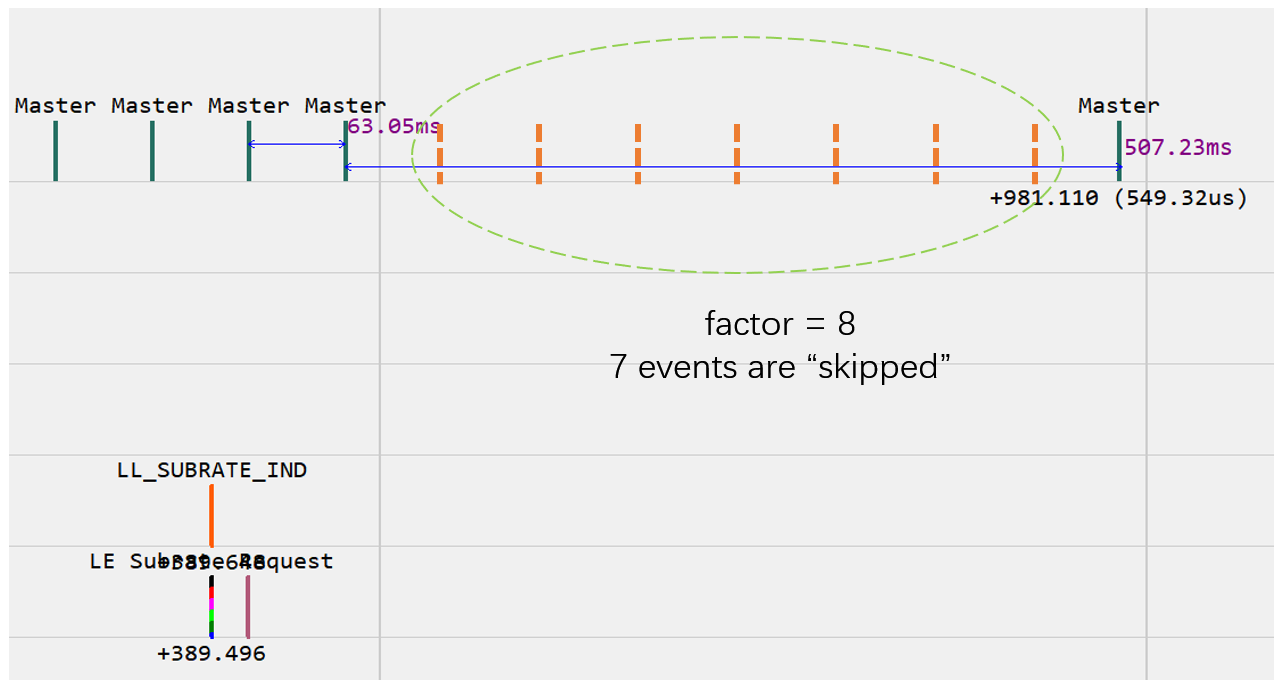
\includegraphics[width=0.85\linewidth]{./img/subrate_start} 

}

\caption{减速比为 8 时的行为}\label{fig:ch2-subrate-8-start}
\end{figure}

\texttt{continuation\_number} 表示每个减速周期开始时,至少再连续传输多少个连接间隔。如果为 1,在上述配置下当双方无数据传输时,每 8 个连接间隔有 2 个激活;
如果为 7,则每个连接间隔有 8 个激活,即都激活。

启用减速模式后,从机延迟的单位从原来的连接间隔变为 (连接间隔 \(\times\) 减速比)。

减速参数更新后,HCI 回调函数会收到 \texttt{HCI\_SUBEVENT\_LE\_SUBRATE\_CHANGE} 事件。

当出现通信需求时,可以迅速从减速模块回到连接通信模式,\textbf{兼顾功耗与效率},如图 \ref{fig:ch2-subrate-8-data}。

\begin{figure}

{\centering 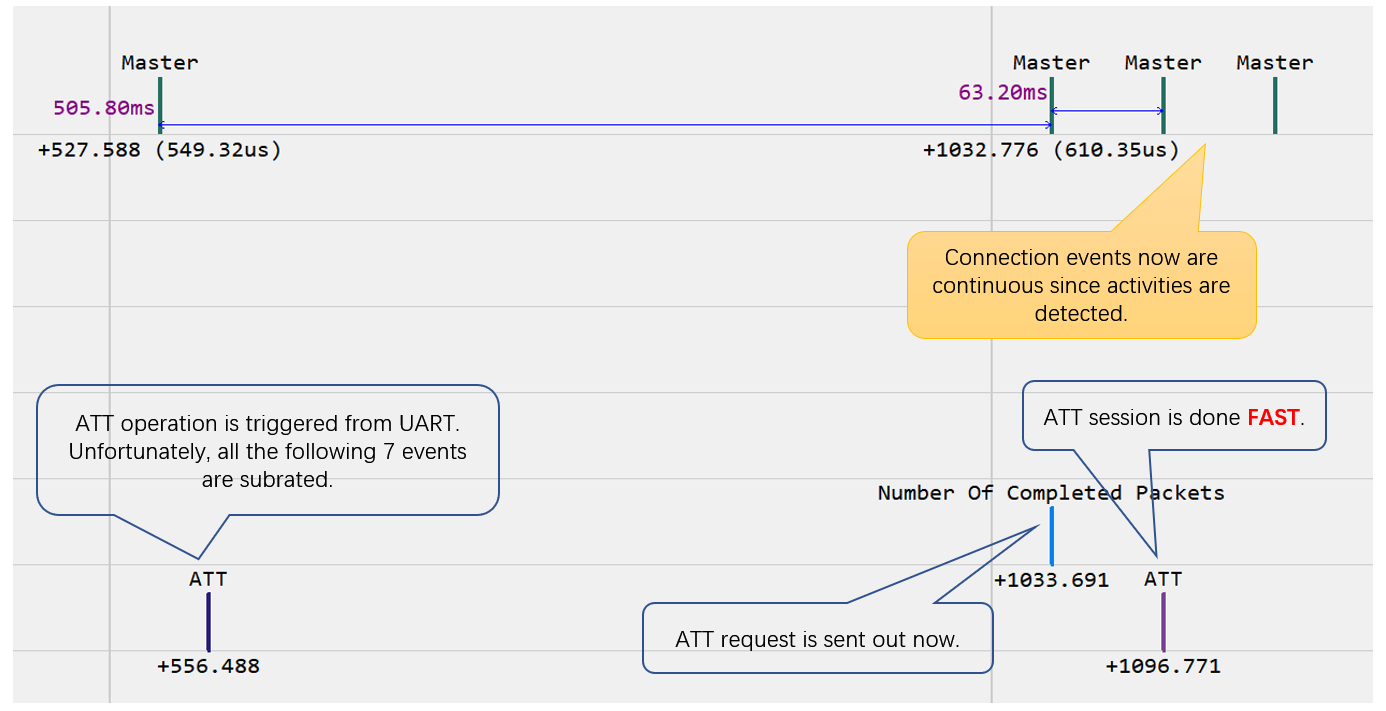
\includegraphics[width=0.85\linewidth]{./img/subrate_att_req} 

}

\caption{减速下出现数据通信}\label{fig:ch2-subrate-8-data}
\end{figure}

通过 \texttt{gap\_set\_default\_subrate} 设置 Controller 所接受的减速模式参数范围。

\begin{Shaded}
\begin{Highlighting}[]
\DataTypeTok{uint8\_t}\NormalTok{ gap\_set\_default\_subrate}\OperatorTok{(}
  \DataTypeTok{uint16\_t}\NormalTok{ subrate\_min}\OperatorTok{,}
  \DataTypeTok{uint16\_t}\NormalTok{ subrate\_max}\OperatorTok{,}
  \DataTypeTok{uint16\_t}\NormalTok{ max\_latency}\OperatorTok{,}
  \DataTypeTok{uint16\_t}\NormalTok{ continuation\_number}\OperatorTok{,}
  \DataTypeTok{uint16\_t}\NormalTok{ supervision\_timeout}\OperatorTok{);}
\end{Highlighting}
\end{Shaded}

\hypertarget{ch-conn-pathloss}{%
\subsection{路损检测与上报}\label{ch-conn-pathloss}}

BLE 5.2 为路径损耗定义了 3 种分类(或者分区,zone),高损耗、中损耗和低损耗。
Controller 监控损耗情况,当损耗分类发生改变时(图 \ref{fig:ch2-path-loss-notification} 中的虚线箭头),上报 HCI\_SUBEVENT\_LE\_PATH\_LOSS\_THRESHOLD 事件。

\begin{figure}

{\centering 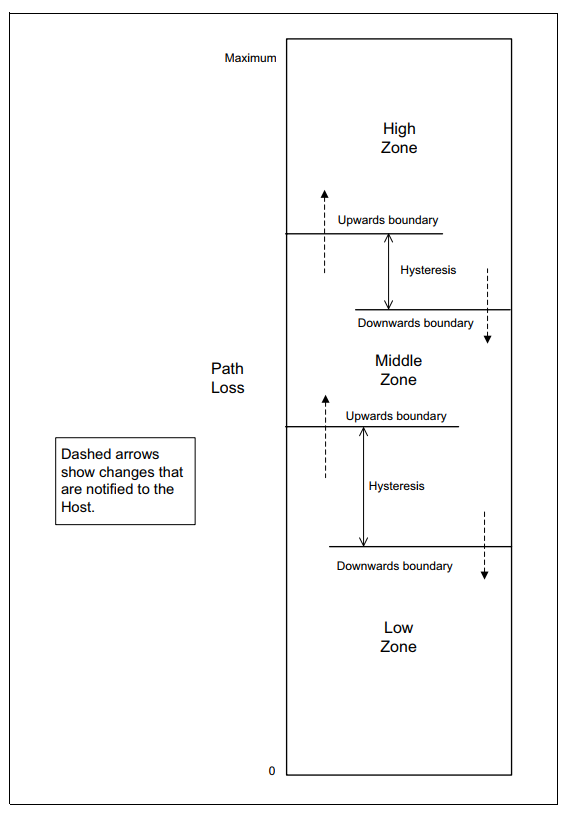
\includegraphics[width=0.6\linewidth]{./img/path_loss_report_zone} 

}

\caption{路径损耗上报}\label{fig:ch2-path-loss-notification}
\end{figure}

\begin{itemize}
\item
  配置路损分类参数:

\begin{Shaded}
\begin{Highlighting}[]
\DataTypeTok{uint8\_t}\NormalTok{ gap\_set\_path\_loss\_reporting\_param}\OperatorTok{(}
\NormalTok{  hci\_con\_handle\_t con\_handle}\OperatorTok{,}  \CommentTok{// 连接句柄}
  \DataTypeTok{uint8\_t}\NormalTok{ high\_threshold}\OperatorTok{,}       \CommentTok{// 高路损门限}
  \DataTypeTok{uint8\_t}\NormalTok{ high\_hysteresis}\OperatorTok{,}      \CommentTok{// 高路损迟滞}
  \DataTypeTok{uint8\_t}\NormalTok{ low\_threshold}\OperatorTok{,}        \CommentTok{// 低路损门限}
  \DataTypeTok{uint8\_t}\NormalTok{ low\_hysteresis}\OperatorTok{,}       \CommentTok{// 低路损迟滞}
  \DataTypeTok{uint8\_t}\NormalTok{ min\_time\_spent}\OperatorTok{);}      \CommentTok{// 最小停留时间(单位连接间隔)}
\end{Highlighting}
\end{Shaded}

  图 \ref{fig:ch2-path-loss-notification} 中的 \emph{upwards boundary} 为 (threshold + hysteresis),
  \emph{downwards boundary} 为 (threshold - hysteresis)。
\item
  使能上报:

\begin{Shaded}
\begin{Highlighting}[]
\DataTypeTok{uint8\_t}\NormalTok{ gap\_set\_path\_loss\_reporting\_enable}\OperatorTok{(}
\NormalTok{  hci\_con\_handle\_t con\_handle}\OperatorTok{,}  \CommentTok{// 连接句柄}
  \DataTypeTok{uint8\_t}\NormalTok{ enable                }\CommentTok{// 使能}
\OperatorTok{);}
\end{Highlighting}
\end{Shaded}
\end{itemize}

\hypertarget{ch-conn-power-ctrl}{%
\subsection{功率控制}\label{ch-conn-power-ctrl}}

功率控制的使用方法可参考 SDK \emph{UART GATT Console}。

\begin{itemize}
\item
  读取发射功率

  读取本端发射功率:

\begin{Shaded}
\begin{Highlighting}[]
\DataTypeTok{uint8\_t}\NormalTok{ gap\_read\_local\_tx\_power\_level}\OperatorTok{(}
\NormalTok{  hci\_con\_handle\_t con\_handle}\OperatorTok{,} \CommentTok{// 连接句柄}
\NormalTok{  unified\_phy\_type\_t phy       }\CommentTok{// PHY}
\OperatorTok{);}
\end{Highlighting}
\end{Shaded}

  从对应的 \texttt{HCI\_EVENT\_COMMAND\_COMPLETE} 事件的返回参数中取得发射功率值:

\begin{Shaded}
\begin{Highlighting}[]
\DataTypeTok{uint8\_t}\NormalTok{ Status}\OperatorTok{,}                 \CommentTok{// 状态码}
\DataTypeTok{uint8\_t}\NormalTok{ Connection\_Handle}\OperatorTok{,}      \CommentTok{// 连接句柄}
\DataTypeTok{uint8\_t}\NormalTok{ PHY}\OperatorTok{,}
 \DataTypeTok{int8\_t}\NormalTok{ Current\_TX\_Power\_Level}\OperatorTok{,} \CommentTok{// 当前发射功率(dBm)}
 \DataTypeTok{int8\_t}\NormalTok{ Max\_TX\_Power\_Level      }\CommentTok{// 最大发射功率(dBm)}
\end{Highlighting}
\end{Shaded}

  读取对端发射功率:

\begin{Shaded}
\begin{Highlighting}[]
\DataTypeTok{uint8\_t}\NormalTok{ gap\_read\_remote\_tx\_power\_level}\OperatorTok{(}
\NormalTok{  hci\_con\_handle\_t con\_handle}\OperatorTok{,} \CommentTok{// 连接句柄}
\NormalTok{  unified\_phy\_type\_t phy       }\CommentTok{// PHY}
\OperatorTok{);}
\end{Highlighting}
\end{Shaded}

  从 \texttt{HCI\_SUBEVENT\_LE\_TRANSMIT\_POWER\_REPORTING} 事件中取得发射功率值。
\item
  设置发射功率

  设置本端发射功率:

\begin{Shaded}
\begin{Highlighting}[]
\DataTypeTok{void}\NormalTok{ ll\_set\_conn\_tx\_power}\OperatorTok{(}
  \DataTypeTok{uint16\_t}\NormalTok{ conn\_handle}\OperatorTok{,} \CommentTok{// 连接句柄}
  \DataTypeTok{int16\_t}\NormalTok{ tx\_power      }\CommentTok{// 发射功率(dBm)}
\OperatorTok{);}
\end{Highlighting}
\end{Shaded}

  调整对端发射功率:

\begin{Shaded}
\begin{Highlighting}[]
\DataTypeTok{void}\NormalTok{ ll\_adjust\_conn\_peer\_tx\_power}\OperatorTok{(}
  \DataTypeTok{uint16\_t}\NormalTok{ conn\_handle}\OperatorTok{,} \CommentTok{// 连接句柄}
  \DataTypeTok{int8\_t}\NormalTok{ delta          }\CommentTok{// 调整量,正值为增大,负值为减小(dB)}
\OperatorTok{);}
\end{Highlighting}
\end{Shaded}
\item
  发射功率自动上报

\begin{Shaded}
\begin{Highlighting}[]

\DataTypeTok{uint8\_t}\NormalTok{ gap\_set\_tx\_power\_reporting\_enable}\OperatorTok{(}
\NormalTok{  hci\_con\_handle\_t con\_handle}\OperatorTok{,}  \CommentTok{// 连接句柄}
  \DataTypeTok{uint8\_t}\NormalTok{ local\_enable}\OperatorTok{,}         \CommentTok{// 使能本端上报}
  \DataTypeTok{uint8\_t}\NormalTok{ remote\_enable         }\CommentTok{// 使能对端上报}
\OperatorTok{);}
\end{Highlighting}
\end{Shaded}
\end{itemize}

\hypertarget{ch-gatt-server}{%
\chapter{GATT - 服务器}\label{ch-gatt-server}}

\hypertarget{ux6982ux89c8-3}{%
\section{概览}\label{ux6982ux89c8-3}}

GATT 服务器\footnote{在不引起混淆的前提下,本手册混用 ATT 服务器、GATT 服务器,代码里也用 \texttt{att\_server} 代指 \texttt{gatt\_server}。}为客户端提供服务。
协议栈支持多个连接,每个连接的配置(Profile)可以独立设置。
需要注意,GATT 服务器和客户端这两个角色与主、从两个角色没有任何关联:一个连接的主角色既可以充当 GATT 的客户端,也可以充当服务器,
还可以两种角色一起扮演;一个连接的从角色也是如此。

要使用 GATT 服务器,开发者需要做三件事\footnote{事实上,这几件事已由 Wizard 工具代劳。}:

\begin{enumerate}
\def\labelenumi{\arabic{enumi}.}
\item
  初试化:设置事件回调

\begin{Shaded}
\begin{Highlighting}[]
\DataTypeTok{void}\NormalTok{ att\_server\_register\_packet\_handler}\OperatorTok{(}
\NormalTok{  btstack\_packet\_handler\_t handler}\OperatorTok{);}
\end{Highlighting}
\end{Shaded}
\item
  初始化:提供回调函数

\begin{Shaded}
\begin{Highlighting}[]
\DataTypeTok{void}\NormalTok{ att\_server\_init}\OperatorTok{(}
  \CommentTok{// 特征的读回调}
\NormalTok{  att\_read\_callback\_t read\_callback}\OperatorTok{,}
  \CommentTok{// 特征的写回调}
\NormalTok{  att\_write\_callback\_t write\_callback}\OperatorTok{);}
\end{Highlighting}
\end{Shaded}

  读回调的类型如下:

\begin{Shaded}
\begin{Highlighting}[]
\KeywordTok{typedef} \DataTypeTok{uint16\_t} \OperatorTok{(*}\NormalTok{att\_read\_callback\_t}\OperatorTok{)(}
  \CommentTok{// 连接句柄}
\NormalTok{  hci\_con\_handle\_t con\_handle}\OperatorTok{,}
  \CommentTok{// 特征句柄}
  \DataTypeTok{uint16\_t}\NormalTok{ attribute\_handle}\OperatorTok{,}
  \CommentTok{// 数据偏移}
  \DataTypeTok{uint16\_t}\NormalTok{ offset}\OperatorTok{,}
  \CommentTok{// 缓存}
  \DataTypeTok{uint8\_t} \OperatorTok{*}\NormalTok{buffer}\OperatorTok{,}
  \CommentTok{// 缓存的大小}
  \DataTypeTok{uint16\_t}\NormalTok{ buffer\_size}\OperatorTok{);}
\end{Highlighting}
\end{Shaded}

  写回调的类型如下:

\begin{Shaded}
\begin{Highlighting}[]
\KeywordTok{typedef} \DataTypeTok{int} \OperatorTok{(*}\NormalTok{att\_write\_callback\_t}\OperatorTok{)(}
  \CommentTok{// 连接句柄}
\NormalTok{  hci\_con\_handle\_t con\_handle}\OperatorTok{,}
  \CommentTok{// 特征句柄}
  \DataTypeTok{uint16\_t}\NormalTok{ attribute\_handle}\OperatorTok{,}
  \CommentTok{// 会话模式}
  \DataTypeTok{uint16\_t}\NormalTok{ transaction\_mode}\OperatorTok{,}
  \CommentTok{// 数据偏移}
  \DataTypeTok{uint16\_t}\NormalTok{ offset}\OperatorTok{,}
  \CommentTok{// 缓存}
  \DataTypeTok{const} \DataTypeTok{uint8\_t} \OperatorTok{*}\NormalTok{buffer}\OperatorTok{,}
  \CommentTok{// 缓存的大小}
  \DataTypeTok{uint16\_t}\NormalTok{ buffer\_size}\OperatorTok{);}
\end{Highlighting}
\end{Shaded}

  将 \texttt{con\_handle} 和 \texttt{attribute\_handle} 组合到一起,回调函数就可以确定是在访问哪个 Profile 里的哪个特征。
  对于长度超过\((ATT\_MTU - 3)\)的长值,BLE 支持分块读写模式,相应地,两个回调函数都有一个 \texttt{offset} 参数。

  关于会话模式 \texttt{transaction\_mode} 的说明见后文。
\item
  适时提供 Profile 数据

\begin{Shaded}
\begin{Highlighting}[]
\DataTypeTok{void}\NormalTok{ att\_set\_db}\OperatorTok{(}
  \CommentTok{// 要关联的句柄}
\NormalTok{  hci\_con\_handle\_t con\_handle}\OperatorTok{,}
  \CommentTok{// Profile 数据库}
  \DataTypeTok{const} \DataTypeTok{uint8\_t} \OperatorTok{*}\NormalTok{db}\OperatorTok{);}
\end{Highlighting}
\end{Shaded}
\end{enumerate}

协议栈内的 GATT 服务器可以通过 2 种方式获得特征的值,然后传输到客户端:

\begin{enumerate}
\def\labelenumi{\arabic{enumi}.}
\item
  保存在 Profile 数据库内部的值

  这种方式适用于值不改变的情况,服务器可能自动将值传输到客户端,不需要开发者参与。
\item
  借助回调函数 \texttt{att\_read\_callback\_t}

  这种方式适用于值动态改变的情况。
  每当客户端读取值时,协议栈会立即调用回调函数,且 \texttt{buffer} 为 \texttt{NULL}。
  这一次调用是为了获取数值长度。回调函数的处理流程又可以分为两种情况:

  \begin{itemize}
  \item
    如果 App 可以立即准备好数据,那么直接返回数值的\textbf{总长};

    之后,协议栈准备内存空间并立即再次调用函数,此时 \texttt{buffer} 参数非 \texttt{NULL},
    回调函数将数据写入 \texttt{buffer} 所指向的内存,读取完成;
  \item
    如果 App 无法立即准备好数据,那么返回 \texttt{ATT\_DEFERRED\_READ} 进入延迟读取模式;

    待数据就绪之后,App 调用 \texttt{att\_server\_deferred\_read\_response} 将数据传给协议栈,读取完成。
  \end{itemize}
\end{enumerate}

每个特性具有若干属性,见表 \ref{tab:ch3-char-properties}。

\begin{longtable}[]{@{}ll@{}}
\caption{\label{tab:ch3-char-properties} 特征的属性}\tabularnewline
\toprule()
属性 & 说明 \\
\midrule()
\endfirsthead
\toprule()
属性 & 说明 \\
\midrule()
\endhead
ATT\_PROPERTY\_BROADCAST & 允许广播该特性的值 \\
ATT\_PROPERTY\_READ & 允许读取 \\
ATT\_PROPERTY\_WRITE\_WITHOUT\_RESPONSE & 允许无响应写入 \\
ATT\_PROPERTY\_WRITE & 允许(有响应的)写入 \\
ATT\_PROPERTY\_NOTIFY & 允许通知(Notification) \\
ATT\_PROPERTY\_INDICATE & 允许指示(Indication) \\
ATT\_PROPERTY\_AUTHENTICATED\_SIGNED\_WRITE & 允许带签名的写入 \\
ATT\_PROPERTY\_EXTENDED\_PROPERTIES & 支持扩展属性 \\
ATT\_PROPERTY\_DYNAMIC & 为动态特性(即需要使用回调函数) \\
\bottomrule()
\end{longtable}

其中 \texttt{DYNAMIC} 为协议栈自定义的属性,只有加上了这个属性,对特性的读写操作才会交由回调函数处理。对于支持写入的特征,
由于总是需要通过回调函数处理,必须加上此属性。

对于支持通知(Notification)和/或指示(Indication)的特征,必须带有 Client Characteristic Configuration
描述符(常被简称为 CCCD):

\begin{itemize}
\tightlist
\item
  将 \texttt{GATT\_CLIENT\_CHARACTERISTICS\_CONFIGURATION\_NOTIFICATION} 写入 CCCD 就可以使能通知,
\item
  将 \texttt{GATT\_CLIENT\_CHARACTERISTICS\_CONFIGURATION\_INDICATION} 写入 CCCD 就可以使能指示,
\item
  将 \texttt{GATT\_CLIENT\_CHARACTERISTICS\_CONFIGURATION\_NONE} 写入 CCCD 就可以关闭通知和指示。
\end{itemize}

通知相当于无响应的上报,而指示相当于有响应的上报。

\hypertarget{ux4f7fux7528ux8bf4ux660e-3}{%
\section{使用说明}\label{ux4f7fux7528ux8bf4ux660e-3}}

\hypertarget{profile-ux6570ux636e}{%
\subsection{Profile 数据}\label{profile-ux6570ux636e}}

Profile 数据\footnote{在手册、工具、代码的不同位置可能使用了不同的名词,如 Profile 数据库、GATT 数据库、GATT 数据等。} 使用了协议栈自定义的数据结构。
开发者不需要了解这个数据结构的定义,而是借助图形化工具或者编程地生成。

\begin{enumerate}
\def\labelenumi{\arabic{enumi}.}
\item
  使用图形化的 Profile 编辑器。

  请参考 《SDK 用户手册》。
\item
  使用 \texttt{att\_db\_util} 模块。

  调用 \texttt{att\_db\_util\_init} 告知 Profile 数据的存储空间。
  调用 \texttt{att\_db\_util\_add\_service\_uuid??} 添加服务,然后通过 \texttt{att\_db\_util\_add\_characteristic\_uuid??} 添加若干特性。
  重复上述步骤可以添加多个服务。最后调用 \texttt{att\_db\_util\_get\_size} 查看整个 Profile 数据的大小,相应调整存储空间的大小,再重新编译程序。

  上面的 \texttt{.....\_uuid??} 函数都包含 \texttt{uuid16} 和 \texttt{uuid128} 等两种形式,分别对应 16-bit 的简短 UUID 和 16 字节的完整 UUID。

  \texttt{att\_db\_util\_add\_characteristic\_uuid??} 函数返回的是特性的值的句柄。
  调用 \texttt{att\_db\_util\_add\_characteristic\_uuid??} 时需要注意根据情况添加 \texttt{ATT\_PROPERTY\_DYNAMIC} 属性。
  对于带有 \texttt{ATT\_PROPERTY\_NOTIFY} 和/或 \texttt{ATT\_PROPERTY\_INDICATE} 属性的特性,\texttt{att\_db\_util\_add\_characteristic\_uuid??} 函数会自动添加 CCCD。
  设特性的值句柄为 \(N\),那么 CCCD 的句柄为 \(N + 1\)。
\end{enumerate}

\hypertarget{ux5b9eux73b0ux8bfbux56deux8c03}{%
\subsection{实现读回调}\label{ux5b9eux73b0ux8bfbux56deux8c03}}

一个典型的读回调函数大概是这种样子:

\begin{Shaded}
\begin{Highlighting}[]
\DataTypeTok{static} \DataTypeTok{uint16\_t}\NormalTok{ att\_read\_callback}\OperatorTok{(}\NormalTok{hci\_con\_handle\_t connection\_handle}\OperatorTok{,}
  \DataTypeTok{uint16\_t}\NormalTok{ att\_handle}\OperatorTok{,} \DataTypeTok{uint16\_t}\NormalTok{ offset}\OperatorTok{,}
  \DataTypeTok{uint8\_t} \OperatorTok{*}\NormalTok{ buffer}\OperatorTok{,} \DataTypeTok{uint16\_t}\NormalTok{ buffer\_size}\OperatorTok{)}
\OperatorTok{\{}
    \ControlFlowTok{switch} \OperatorTok{(}\NormalTok{att\_handle}\OperatorTok{)}
    \OperatorTok{\{}
    \ControlFlowTok{case}\NormalTok{ HANDLE\_0}\OperatorTok{:}
        \ControlFlowTok{if} \OperatorTok{(}\NormalTok{buffer}\OperatorTok{)}
        \OperatorTok{\{}
\NormalTok{            memcpy}\OperatorTok{(}\NormalTok{buffer}\OperatorTok{,} \OperatorTok{...)}
            \ControlFlowTok{return}\NormalTok{ buffer\_size}\OperatorTok{;}
        \OperatorTok{\}}
        \ControlFlowTok{else}
            \ControlFlowTok{return}\NormalTok{ size of value}\OperatorTok{;}
    \CommentTok{//...}
    \ControlFlowTok{default}\OperatorTok{:}
        \ControlFlowTok{return} \DecValTok{0}\OperatorTok{;}
    \OperatorTok{\}}
\OperatorTok{\}}
\end{Highlighting}
\end{Shaded}

延迟读取的情况:

\begin{Shaded}
\begin{Highlighting}[]
\DataTypeTok{static} \DataTypeTok{uint16\_t}\NormalTok{ att\_read\_callback}\OperatorTok{(}\NormalTok{hci\_con\_handle\_t connection\_handle}\OperatorTok{,}
  \DataTypeTok{uint16\_t}\NormalTok{ att\_handle}\OperatorTok{,} \DataTypeTok{uint16\_t}\NormalTok{ offset}\OperatorTok{,}
  \DataTypeTok{uint8\_t} \OperatorTok{*}\NormalTok{ buffer}\OperatorTok{,} \DataTypeTok{uint16\_t}\NormalTok{ buffer\_size}\OperatorTok{)}
\OperatorTok{\{}
    \ControlFlowTok{switch} \OperatorTok{(}\NormalTok{att\_handle}\OperatorTok{)}
    \OperatorTok{\{}
    \ControlFlowTok{case}\NormalTok{ HANDLE\_0}\OperatorTok{:}
        \CommentTok{//...}
        \ControlFlowTok{return}\NormalTok{ ATT\_DEFERRED\_READ}\OperatorTok{;}
    \CommentTok{//...}
    \ControlFlowTok{default}\OperatorTok{:}
        \ControlFlowTok{return} \DecValTok{0}\OperatorTok{;}
    \OperatorTok{\}}
\OperatorTok{\}}
\end{Highlighting}
\end{Shaded}

延迟读取的数据通过 \texttt{att\_server\_deferred\_read\_response} 传递给协议栈:

\begin{Shaded}
\begin{Highlighting}[]
\DataTypeTok{int}\NormalTok{ att\_server\_deferred\_read\_response}\OperatorTok{(}
  \CommentTok{// 连接句柄}
\NormalTok{  hci\_con\_handle\_t con\_handle}\OperatorTok{,}
  \CommentTok{// 特征句柄}
  \DataTypeTok{uint16\_t}\NormalTok{ attribute\_handle}\OperatorTok{,}
  \CommentTok{// 指向值的指针}
  \DataTypeTok{const} \DataTypeTok{uint8\_t} \OperatorTok{*}\NormalTok{value}\OperatorTok{,}
  \CommentTok{// 值的长度}
  \DataTypeTok{uint16\_t}\NormalTok{ value\_len}\OperatorTok{);}
\end{Highlighting}
\end{Shaded}

SDK \emph{GATT Relay} 演示了延迟读取的具体用法。

\hypertarget{ux5b9eux73b0ux5199ux56deux8c03}{%
\subsection{实现写回调}\label{ux5b9eux73b0ux5199ux56deux8c03}}

当写特性时,可能触发服务器执行某个动作。BLE 为了精度控制动作的执行引入了会话\footnote{协议栈里称为``会话'',规范里称为``队列''。}概念:
一个会话包含对 1 个或多个特性的写入,最后是一个显式的``执行''命令通知服务器开始执行。此外还有一个``取消''命令,通知服务器会话不要执行动作、直接终止。相应地,
写回调的会话模式 \texttt{transaction\_mode} 参数包含四种值:

\begin{Shaded}
\begin{Highlighting}[]
\CommentTok{// 无会话的普通写入}
\PreprocessorTok{\#define ATT\_TRANSACTION\_MODE\_NONE      ...}
\CommentTok{// 带会话的写入}
\PreprocessorTok{\#define ATT\_TRANSACTION\_MODE\_ACTIVE    ...}
\CommentTok{// 执行}
\PreprocessorTok{\#define ATT\_TRANSACTION\_MODE\_EXECUTE   ...}
\CommentTok{// 取消}
\PreprocessorTok{\#define ATT\_TRANSACTION\_MODE\_CANCEL    ...}
\end{Highlighting}
\end{Shaded}

对于 \texttt{NONE} 和 \texttt{ACTIVE} 两种模式,都会传入要写入的数据,而 \texttt{EXECUTE} 和 \texttt{CANCEL} 则既不会传入特征句柄,也不传入数据,
也就是说这两个命令只关联到连接,施加于整个服务器,而不针对某个特征。

一个典型的写回调函数大概是这种样子:

\begin{Shaded}
\begin{Highlighting}[]
\DataTypeTok{static} \DataTypeTok{int}\NormalTok{ att\_write\_callback}\OperatorTok{(}
\NormalTok{  hci\_con\_handle\_t connection\_handle}\OperatorTok{,} \DataTypeTok{uint16\_t}\NormalTok{ att\_handle}\OperatorTok{,}
  \DataTypeTok{uint16\_t}\NormalTok{ transaction\_mode}\OperatorTok{,}
  \DataTypeTok{uint16\_t}\NormalTok{ offset}\OperatorTok{,} \DataTypeTok{const} \DataTypeTok{uint8\_t} \OperatorTok{*}\NormalTok{buffer}\OperatorTok{,} \DataTypeTok{uint16\_t}\NormalTok{ buffer\_size}\OperatorTok{)}
\OperatorTok{\{}
\NormalTok{    处理 EXECUTE 和 CANCEL 两种会话模式并返回}\OperatorTok{;}

    \CommentTok{//}
    \ControlFlowTok{switch} \OperatorTok{(}\NormalTok{att\_handle}\OperatorTok{)}
    \OperatorTok{\{}
    \ControlFlowTok{case}\NormalTok{ HANDLE\_0}\OperatorTok{:}
        \CommentTok{//...}
        \ControlFlowTok{return} \DecValTok{0}\OperatorTok{;}
    \CommentTok{//...}
    \ControlFlowTok{default}\OperatorTok{:}
        \ControlFlowTok{return} \DecValTok{0}\OperatorTok{;}
    \OperatorTok{\}}
\OperatorTok{\}}
\end{Highlighting}
\end{Shaded}

如果发现错误,可以返回非 0 值告知客户端\footnote{仅适用于有响应的写入,无响应的写入无效。}。

\hypertarget{ux53d1ux9001ux901aux77e5notification}{%
\subsection{发送通知(Notification)}\label{ux53d1ux9001ux901aux77e5notification}}

通过 \texttt{att\_server\_notify} 发送通知:

\begin{Shaded}
\begin{Highlighting}[]
\DataTypeTok{int}\NormalTok{ att\_server\_notify}\OperatorTok{(}
  \CommentTok{// 连接句柄}
\NormalTok{  hci\_con\_handle\_t con\_handle}\OperatorTok{,}
  \CommentTok{// 特征句柄}
  \DataTypeTok{uint16\_t}\NormalTok{ attribute\_handle}\OperatorTok{,}
  \CommentTok{// 指向值的指针}
  \DataTypeTok{const} \DataTypeTok{uint8\_t} \OperatorTok{*}\NormalTok{value}\OperatorTok{,}
  \CommentTok{// 值的长度}
  \DataTypeTok{uint16\_t}\NormalTok{ value\_len}\OperatorTok{);}
\end{Highlighting}
\end{Shaded}

\hypertarget{ux53d1ux9001ux6307ux793aindication}{%
\subsection{发送指示(Indication)}\label{ux53d1ux9001ux6307ux793aindication}}

通过 \texttt{att\_server\_indicate} 发送指示:

\begin{Shaded}
\begin{Highlighting}[]
\DataTypeTok{int}\NormalTok{ att\_server\_indicate}\OperatorTok{(}
  \CommentTok{// 连接句柄}
\NormalTok{  hci\_con\_handle\_t con\_handle}\OperatorTok{,}
  \CommentTok{// 特征句柄}
  \DataTypeTok{uint16\_t}\NormalTok{ attribute\_handle}\OperatorTok{,}
  \CommentTok{// 指向值的指针}
  \DataTypeTok{const} \DataTypeTok{uint8\_t} \OperatorTok{*}\NormalTok{value}\OperatorTok{,}
  \CommentTok{// 值的长度}
  \DataTypeTok{uint16\_t}\NormalTok{ value\_len}\OperatorTok{);}
\end{Highlighting}
\end{Shaded}

指示的响应通过 \texttt{ATT\_EVENT\_HANDLE\_VALUE\_INDICATION\_COMPLETE} 事件通知 App。

\begin{rmdcaution}
在收到 \texttt{ATT\_EVENT\_HANDLE\_VALUE\_INDICATION\_COMPLETE}
事件前,不能发送新的指示,否则 \texttt{att\_server\_indicate}
将返回错误码 \texttt{ATT\_HANDLE\_VALUE\_INDICATION\_IN\_PORGRESS}。
\end{rmdcaution}

\hypertarget{ux54cdux5e94ux4e8bux4ef6}{%
\subsection{响应事件}\label{ux54cdux5e94ux4e8bux4ef6}}

GATT 服务器模块会弹出以下事件。

\begin{itemize}
\item
  \texttt{ATT\_EVENT\_MTU\_EXCHANGE\_COMPLETE}

  这个事件表示 MTU 协商完成。有两个解析函数:

  \begin{itemize}
  \tightlist
  \item
    \texttt{att\_event\_mtu\_exchange\_complete\_get\_handle(packet)}
    获得连接句柄;
  \item
    \texttt{att\_event\_mtu\_exchange\_complete\_get\_MTU(packet)}
    获得 MTU 大小。
  \end{itemize}
\item
  \texttt{ATT\_EVENT\_HANDLE\_VALUE\_INDICATION\_COMPLETE}

  这个事件表示指示发送完成。有三个解析函数:

  \begin{itemize}
  \item
    \texttt{att\_event\_handle\_value\_indication\_complete\_get\_conn\_handle(packet)}
    获得连接句柄;
  \item
    \texttt{att\_event\_handle\_value\_indication\_complete\_get\_attribute\_handle(packet)}
    获得特征句柄;
  \item
    \texttt{att\_event\_handle\_value\_indication\_complete\_get\_status(packet)}
    获得响应状态。

    共有两种状态:\(0\) 表示成功送达,\texttt{ATT\_HANDLE\_VALUE\_INDICATION\_TIMEOUT} 表示超时。
  \end{itemize}
\end{itemize}

\hypertarget{att_mtu}{%
\subsection{ATT\_MTU}\label{att_mtu}}

除了通过监听 \texttt{ATT\_EVENT\_MTU\_EXCHANGE\_COMPLETE} 事件以外,通过 \texttt{att\_server\_get\_mtu} 可以随时获取 ATT\_MTU:

\begin{Shaded}
\begin{Highlighting}[]
\DataTypeTok{uint16\_t}\NormalTok{ att\_server\_get\_mtu}\OperatorTok{(}
  \CommentTok{// 连接句柄}
\NormalTok{  hci\_con\_handle\_t con\_handle}\OperatorTok{);}
\end{Highlighting}
\end{Shaded}

特征的值的最大长度为 \((ATT\_MTU - 3)\)。调用 \texttt{att\_server\_indicate} 或 \texttt{att\_server\_notify} 上报数据时,
如果超过最大长度,会被自动截短。

\hypertarget{ch-gatt-client}{%
\chapter{GATT - 客户端}\label{ch-gatt-client}}

\hypertarget{ux6982ux89c8-4}{%
\section{概览}\label{ux6982ux89c8-4}}

GATT 客户端的主要功能是发现服务,读写和订阅特征。每个连接使用独立的 GATT 客户端实例。

GATT 客户端的操作几乎都需要先发出数据再等待服务器发回响应,需要较长的时间,所以也引入了会话的概念:
如果上一个会话未结束,那么就不允许发起新的会话。每次发起会话时,都要提供一个专门的回调函数。
当这个回调函数收到 \texttt{GATT\_EVENT\_QUERY\_COMPLETE} 事件时,会话结束。

使用 GATT 客户端 API 时需要注意检查返回值,常见的返回值有:

\begin{itemize}
\item
  \(0\):正常、成功;
\item
  \texttt{BTSTACK\_MEMORY\_ALLOC\_FAILED}:内存不足,无法创建 GATT 客户端实例
\item
  \texttt{GATT\_CLIENT\_IN\_WRONG\_STATE}:会话冲突

  解决方法:等待上一个会话完成后再发起新的会话。通过 \texttt{gatt\_client\_is\_ready} 可以查询当前是否可以发起新的会话。
\item
  \texttt{GATT\_CLIENT\_VALUE\_TOO\_LONG}:要写入的值超出 MTU 的限制

  解决方法:缩短值的长度;或者检查对比设备的 MTU 能力。
\end{itemize}

可选地,开发者可以设置 GATT 客户端事件回调:

\begin{Shaded}
\begin{Highlighting}[]
\DataTypeTok{void}\NormalTok{ gatt\_client\_register\_handler}\OperatorTok{(}
\NormalTok{  btstack\_packet\_handler\_t handler}\OperatorTok{);}
\end{Highlighting}
\end{Shaded}

这个回调函数目前只会收到一个事件\footnote{以及转发过来的 \texttt{L2CAP\_EVENT\_CAN\_SEND\_NOW} 事件。}:

\begin{itemize}
\item
  \texttt{GATT\_EVENT\_MTU}

  这个事件表示 MTU 协商完成。有两个解析函数:

  \begin{itemize}
  \item
    \texttt{gatt\_event\_mtu\_get\_handle(packet)}

    获得连接句柄;
  \item
    \texttt{gatt\_event\_mtu\_get\_mtu(packet)}

    获得 MTU 大小。
  \end{itemize}
\end{itemize}

\hypertarget{ux53e5ux67c4ux8303ux56f4}{%
\subsection{句柄范围}\label{ux53e5ux67c4ux8303ux56f4}}

特征包含值和若干个描述符,每个描述符也对应于一个句柄,所以一个特征包含从 \texttt{start\_handle} 到 \texttt{end\_handle} 的一系列句柄。
同理,服务也对应一个句柄范围。

本章在不引起误解的前提下,把特征的值的句柄简称为``特征的句柄''。

\hypertarget{ux4f7fux7528ux8bf4ux660e-4}{%
\section{使用说明}\label{ux4f7fux7528ux8bf4ux660e-4}}

\hypertarget{ux521bux5efaux5ba2ux6237ux7aef}{%
\subsection{创建客户端}\label{ux521bux5efaux5ba2ux6237ux7aef}}

调用 GATT 客户端的绝大多数 API 时,都会按需自动创建客户端实例。不会触发创建动作的 API:

\begin{itemize}
\tightlist
\item
  \texttt{gatt\_client\_listen\_for\_characteristic\_value\_updates}
\end{itemize}

通过 \texttt{gatt\_client\_is\_ready()} 可``手动''创建客户端实例。

\hypertarget{ux53d1ux73b0ux670dux52a1}{%
\subsection{发现服务}\label{ux53d1ux73b0ux670dux52a1}}

下列 API 用来发现服务:

\begin{itemize}
\item
  \texttt{gatt\_client\_discover\_primary\_services}:发现所有服务。
\item
  \texttt{gatt\_client\_discover\_primary\_services\_by\_uuid16}:发现指定的服务。
\item
  \texttt{gatt\_client\_discover\_primary\_services\_by\_uuid128}:发现指定的服务。
\end{itemize}

下列 API 用来发现服务内部的特征:

\begin{itemize}
\item
  \texttt{gatt\_client\_discover\_characteristics\_for\_service}:发现一个服务里的所有特征
\item
  \texttt{gatt\_client\_discover\_characteristics\_for\_handle\_range\_by\_uuid16}:在一定句柄范围内发现指定的特征
\item
  \texttt{gatt\_client\_discover\_characteristics\_for\_handle\_range\_by\_uuid16}:在一定句柄范围内发现指定的特征
\item
  \texttt{gatt\_client\_discover\_characteristic\_descriptors}:发现特征的所有描述符。
\end{itemize}

以 \texttt{gatt\_client\_discover\_primary\_services} 的使用为例说明使用方法。这个 API 的原型如下:

\begin{Shaded}
\begin{Highlighting}[]
\DataTypeTok{uint8\_t}\NormalTok{ gatt\_client\_discover\_primary\_services}\OperatorTok{(}
  \CommentTok{// 回调}
\NormalTok{  user\_packet\_handler\_t callback}\OperatorTok{,}
  \CommentTok{// 连接句柄}
\NormalTok{  hci\_con\_handle\_t con\_handle}\OperatorTok{);}
\end{Highlighting}
\end{Shaded}

其回调函数的例子:

\begin{Shaded}
\begin{Highlighting}[]
\DataTypeTok{static} \DataTypeTok{void}\NormalTok{ service\_discovery\_callback}\OperatorTok{(}
  \CommentTok{// 事件包类型(忽略)}
  \DataTypeTok{uint8\_t}\NormalTok{ packet\_type}\OperatorTok{,}
  \CommentTok{// 连接句柄(这个句柄也可以从事件内部获得,故忽略此参数)}
  \DataTypeTok{uint16\_t}\NormalTok{ \_}\OperatorTok{,}
  \CommentTok{// 事件包}
  \DataTypeTok{const} \DataTypeTok{uint8\_t} \OperatorTok{*}\NormalTok{packet}\OperatorTok{,}
  \CommentTok{// 事件包大小}
  \DataTypeTok{uint16\_t}\NormalTok{ size}\OperatorTok{)}
\OperatorTok{\{}
    \DataTypeTok{uint16\_t}\NormalTok{ con\_handle}\OperatorTok{;}
    \ControlFlowTok{switch} \OperatorTok{(}\NormalTok{packet}\OperatorTok{[}\DecValTok{0}\OperatorTok{])}
    \OperatorTok{\{}
    \CommentTok{// 对于发现的每个服务都有一个 QUERY\_RESULT}
    \ControlFlowTok{case}\NormalTok{ GATT\_EVENT\_SERVICE\_QUERY\_RESULT}\OperatorTok{:}
        \OperatorTok{\{}
            \DataTypeTok{const}\NormalTok{ gatt\_event\_service\_query\_result\_t }\OperatorTok{*}\NormalTok{result }\OperatorTok{=}
\NormalTok{                gatt\_event\_service\_query\_result\_parse}\OperatorTok{(}\NormalTok{packet}\OperatorTok{);}
            \CommentTok{// ....}
        \OperatorTok{\}}
        \ControlFlowTok{break}\OperatorTok{;}
    \ControlFlowTok{case}\NormalTok{ GATT\_EVENT\_QUERY\_COMPLETE}\OperatorTok{:}
        \CommentTok{// 会话完成}
        \ControlFlowTok{break}\OperatorTok{;}
    \OperatorTok{\}}
\OperatorTok{\}}
\end{Highlighting}
\end{Shaded}

为了简化开发,SDK 提供了 \emph{gatt\_client\_util} 模块,只调用一个函数就可以完成服务发现:

\begin{Shaded}
\begin{Highlighting}[]
\KeywordTok{struct}\NormalTok{ gatt\_client\_discoverer }\OperatorTok{*}\NormalTok{gatt\_client\_util\_discover\_all}\OperatorTok{(}
    \CommentTok{// 连接句柄}
\NormalTok{    hci\_con\_handle\_t con\_handle}\OperatorTok{,}
    \CommentTok{// 发现完成后的回调}
\NormalTok{    f\_on\_fully\_discovered on\_fully\_discovered}\OperatorTok{,}
    \CommentTok{// 传递给黑调的用户数据}
    \DataTypeTok{void} \OperatorTok{*}\NormalTok{user\_data}\OperatorTok{);}
\end{Highlighting}
\end{Shaded}

下面的回调函数演示了如何遍历所有服务、特征:

\begin{Shaded}
\begin{Highlighting}[]
\DataTypeTok{void}\NormalTok{ my\_on\_fully\_discovered}\OperatorTok{(}
    \CommentTok{// 第一个服务}
\NormalTok{    service\_node\_t }\OperatorTok{*}\NormalTok{first}\OperatorTok{,}
    \CommentTok{// 用户数据}
    \DataTypeTok{void} \OperatorTok{*}\NormalTok{user\_data}\OperatorTok{,}
    \CommentTok{// 错误码}
    \DataTypeTok{int}\NormalTok{ err\_code}\OperatorTok{)}
\OperatorTok{\{}
    \ControlFlowTok{if} \OperatorTok{(}\NormalTok{err\_code}\OperatorTok{)} \OperatorTok{...}
\NormalTok{    service\_node\_t }\OperatorTok{*}\NormalTok{s }\OperatorTok{=}\NormalTok{ first}\OperatorTok{;}
    \CommentTok{// 遍历服务}
    \ControlFlowTok{while} \OperatorTok{(}\NormalTok{s}\OperatorTok{)}
    \OperatorTok{\{}
\NormalTok{        char\_node\_t }\OperatorTok{*}\NormalTok{c }\OperatorTok{=}\NormalTok{ s}\OperatorTok{{-}\textgreater{}}\NormalTok{chars}\OperatorTok{;}
        \CommentTok{// 遍历服务的所有特征}
        \ControlFlowTok{while} \OperatorTok{(}\NormalTok{c}\OperatorTok{)}
        \OperatorTok{\{}
\NormalTok{            desc\_node\_t }\OperatorTok{*}\NormalTok{d }\OperatorTok{=}\NormalTok{ c}\OperatorTok{{-}\textgreater{}}\NormalTok{descs}\OperatorTok{;}
            \CommentTok{// 遍历特征的所有描述符}
            \ControlFlowTok{while} \OperatorTok{(}\NormalTok{d}\OperatorTok{)}
            \OperatorTok{\{}
\NormalTok{                d }\OperatorTok{=}\NormalTok{ d}\OperatorTok{{-}\textgreater{}}\NormalTok{next}\OperatorTok{;}
            \OperatorTok{\}}
\NormalTok{            c }\OperatorTok{=}\NormalTok{ c}\OperatorTok{{-}\textgreater{}}\NormalTok{next}\OperatorTok{;}
        \OperatorTok{\}}
\NormalTok{        s }\OperatorTok{=}\NormalTok{ s}\OperatorTok{{-}\textgreater{}}\NormalTok{next}\OperatorTok{;}
    \OperatorTok{\}}
\OperatorTok{\}}
\end{Highlighting}
\end{Shaded}

\hypertarget{ux8bfbux53d6ux7279ux5f81}{%
\subsection{读取特征}\label{ux8bfbux53d6ux7279ux5f81}}

可以通过特征的句柄或者 UUID 读取值:

\begin{itemize}
\tightlist
\item
  \texttt{gatt\_client\_read\_value\_of\_characteristic\_using\_value\_handle}
\item
  \texttt{gatt\_client\_read\_value\_of\_characteristics\_by\_uuid16}
\item
  \texttt{gatt\_client\_read\_value\_of\_characteristics\_by\_uuid128}
\end{itemize}

也可以指定多个句柄批量读取:

\begin{itemize}
\tightlist
\item
  \texttt{gatt\_client\_read\_multiple\_characteristic\_values}
\end{itemize}

基于句柄的分块读取:

\begin{itemize}
\tightlist
\item
  \texttt{gatt\_client\_read\_long\_value\_of\_characteristic\_using\_value\_handle}
\item
  \texttt{gatt\_client\_read\_long\_value\_of\_characteristic\_using\_value\_handle\_with\_offset}
\end{itemize}

以 \texttt{gatt\_client\_read\_value\_of\_characteristic\_using\_value\_handle} 说明使用方法。其原型为:

\begin{Shaded}
\begin{Highlighting}[]
\DataTypeTok{uint8\_t}\NormalTok{ gatt\_client\_read\_value\_of\_characteristic\_using\_value\_handle}\OperatorTok{(}
  \CommentTok{// 回调}
\NormalTok{  btstack\_packet\_handler\_t callback}\OperatorTok{,}
  \CommentTok{// 连接句柄}
\NormalTok{  hci\_con\_handle\_t con\_handle}\OperatorTok{,}
  \CommentTok{// 特征句柄}
  \DataTypeTok{uint16\_t}\NormalTok{ characteristic\_value\_handle}\OperatorTok{);}
\end{Highlighting}
\end{Shaded}

其回调函数的例子:

\begin{Shaded}
\begin{Highlighting}[]
\DataTypeTok{void}\NormalTok{ read\_characteristic\_value\_callback}\OperatorTok{(}
  \CommentTok{// 事件包类型(忽略)}
  \DataTypeTok{uint8\_t}\NormalTok{ packet\_type}\OperatorTok{,}
  \CommentTok{// 连接句柄(这个句柄也可以从事件内部获得,故忽略此参数)}
  \DataTypeTok{uint16\_t}\NormalTok{ \_}\OperatorTok{,}
  \CommentTok{// 事件包}
  \DataTypeTok{const} \DataTypeTok{uint8\_t} \OperatorTok{*}\NormalTok{packet}\OperatorTok{,}
  \CommentTok{// 事件包大小}
  \DataTypeTok{uint16\_t}\NormalTok{ size}\OperatorTok{)}
\OperatorTok{\{}
    \ControlFlowTok{switch} \OperatorTok{(}\NormalTok{packet}\OperatorTok{[}\DecValTok{0}\OperatorTok{])}
    \OperatorTok{\{}
    \ControlFlowTok{case}\NormalTok{ GATT\_EVENT\_CHARACTERISTIC\_VALUE\_QUERY\_RESULT}\OperatorTok{:}
        \OperatorTok{\{}
            \DataTypeTok{uint16\_t}\NormalTok{ value\_size}\OperatorTok{;}
            \DataTypeTok{const}\NormalTok{ gatt\_event\_value\_packet\_t }\OperatorTok{*}\NormalTok{value }\OperatorTok{=}
\NormalTok{                gatt\_event\_characteristic\_value\_query\_result\_parse}\OperatorTok{(}
\NormalTok{                  packet}\OperatorTok{,}\NormalTok{ size}\OperatorTok{,} \OperatorTok{\&}\NormalTok{value\_size}\OperatorTok{);}
            \CommentTok{// value{-}\textgreater{}handle 为特征句柄}
            \CommentTok{// value\_size 为值的长度}
            \CommentTok{// value{-}\textgreater{}value 是指向值的指针}
        \OperatorTok{\}}
        \ControlFlowTok{break}\OperatorTok{;}
    \ControlFlowTok{case}\NormalTok{ GATT\_EVENT\_QUERY\_COMPLETE}\OperatorTok{:}
        \CommentTok{// 会话完成}
        \ControlFlowTok{break}\OperatorTok{;}
    \OperatorTok{\}}
\OperatorTok{\}}
\end{Highlighting}
\end{Shaded}

\hypertarget{ux5199ux5165ux7279ux5f81}{%
\subsection{写入特征}\label{ux5199ux5165ux7279ux5f81}}

通过特征的句柄写入值:

\begin{itemize}
\tightlist
\item
  \texttt{gatt\_client\_write\_value\_of\_characteristic}:有响应的写入
\item
  \texttt{gatt\_client\_write\_value\_of\_characteristic\_without\_response}:无响应的写入
\end{itemize}

基于句柄的分块写入:

\begin{itemize}
\tightlist
\item
  \texttt{gatt\_client\_write\_long\_value\_of\_characteristic}
\item
  \texttt{gatt\_client\_write\_long\_value\_of\_characteristic\_with\_offset}
\end{itemize}

其中 \texttt{gatt\_client\_write\_value\_of\_characteristic} 的原型为:

\begin{Shaded}
\begin{Highlighting}[]
\DataTypeTok{uint8\_t}\NormalTok{ gatt\_client\_write\_value\_of\_characteristic}\OperatorTok{(}
    \CommentTok{// 回调}
\NormalTok{    btstack\_packet\_handler\_t callback}\OperatorTok{,}
    \CommentTok{// 连接句柄}
\NormalTok{    hci\_con\_handle\_t con\_handle}\OperatorTok{,}
    \CommentTok{// 特征句柄}
    \DataTypeTok{uint16\_t}\NormalTok{ characteristic\_value\_handle}\OperatorTok{,}
    \CommentTok{// 值的长度}
    \DataTypeTok{uint16\_t}\NormalTok{ length}\OperatorTok{,}
    \CommentTok{// 指向值的指针}
    \DataTypeTok{const} \DataTypeTok{uint8\_t} \OperatorTok{*}\NormalTok{ data}\OperatorTok{);}
\end{Highlighting}
\end{Shaded}

其回调函数的例子:

\begin{Shaded}
\begin{Highlighting}[]
\DataTypeTok{void}\NormalTok{ write\_characteristic\_value\_callback}\OperatorTok{(}
    \DataTypeTok{uint8\_t}\NormalTok{ packet\_type}\OperatorTok{,} \DataTypeTok{uint16\_t}\NormalTok{ \_}\OperatorTok{,}
    \DataTypeTok{const} \DataTypeTok{uint8\_t} \OperatorTok{*}\NormalTok{packet}\OperatorTok{,} \DataTypeTok{uint16\_t}\NormalTok{ size}\OperatorTok{)}
\OperatorTok{\{}
    \ControlFlowTok{switch} \OperatorTok{(}\NormalTok{packet}\OperatorTok{[}\DecValTok{0}\OperatorTok{])}
    \OperatorTok{\{}
    \ControlFlowTok{case}\NormalTok{ GATT\_EVENT\_QUERY\_COMPLETE}\OperatorTok{:}
\NormalTok{        platform\_printf}\OperatorTok{(}\StringTok{"特征写入完成。状态码:: \%d}\SpecialCharTok{\textbackslash{}n}\StringTok{"}\OperatorTok{,}
\NormalTok{            gatt\_event\_query\_complete\_parse}\OperatorTok{(}\NormalTok{packet}\OperatorTok{){-}\textgreater{}}\NormalTok{status}\OperatorTok{);}
        \ControlFlowTok{break}\OperatorTok{;}
    \OperatorTok{\}}
\OperatorTok{\}}
\end{Highlighting}
\end{Shaded}

与之相比,无响应的写入不需要提供回调函数,没有``会话''的概念,下一次写入不需要等待上次完成,数据吞吐率更高。

\begin{Shaded}
\begin{Highlighting}[]
\DataTypeTok{uint8\_t}\NormalTok{ gatt\_client\_write\_value\_of\_characteristic\_without\_response}\OperatorTok{(}
    \CommentTok{// 连接句柄}
\NormalTok{    hci\_con\_handle\_t con\_handle}\OperatorTok{,}
    \CommentTok{// 特征句柄}
    \DataTypeTok{uint16\_t}\NormalTok{ characteristic\_value\_handle}\OperatorTok{,}
    \CommentTok{// 值的长度}
    \DataTypeTok{uint16\_t}\NormalTok{ length}\OperatorTok{,}
    \CommentTok{// 指向值的指针}
    \DataTypeTok{const} \DataTypeTok{uint8\_t} \OperatorTok{*}\NormalTok{ data}\OperatorTok{);}
\end{Highlighting}
\end{Shaded}

\hypertarget{ux8ba2ux9605ux7279ux5f81}{%
\subsection{订阅特征}\label{ux8ba2ux9605ux7279ux5f81}}

开发者需要完成两个步骤:

\begin{enumerate}
\def\labelenumi{\arabic{enumi}.}
\item
  调用 \texttt{gatt\_client\_listen\_for\_characteristic\_value\_updates} 添加值更新时的回调函数

\begin{Shaded}
\begin{Highlighting}[]
\DataTypeTok{void}\NormalTok{ gatt\_client\_listen\_for\_characteristic\_value\_updates}\OperatorTok{(}
    \CommentTok{// 开发者提供一个回调函数结构体}
\NormalTok{    gatt\_client\_notification\_t }\OperatorTok{*}\NormalTok{ notification}\OperatorTok{,}
    \CommentTok{// 回调函数}
\NormalTok{    btstack\_packet\_handler\_t packet\_handler}\OperatorTok{,}
    \CommentTok{// 连接句柄}
\NormalTok{    hci\_con\_handle\_t con\_handle}\OperatorTok{,}
    \CommentTok{// 特征的值的句柄}
    \DataTypeTok{uint16\_t}\NormalTok{ value\_handle}\OperatorTok{);}
\end{Highlighting}
\end{Shaded}

  由于 \texttt{notification} 会被添加到 GATT 客户端实例的回调链表中,所以必须指向一块全局内存,一定\textbf{不能}在栈上分配。\texttt{notification} 所指向的内容不需要初始化。

  \begin{rmdcaution}
   如果 notification
   是从动态内存(如堆)里分配的,那么当连接断开时记得释放这块内存,以免泄露。
   \end{rmdcaution}
\item
  调用 \texttt{gatt\_client\_write\_characteristic\_descriptor\_using\_descriptor\_handle} 向 CCCD 写入使能标志

  这个函数的原型及使用方法与 \texttt{gatt\_client\_write\_value\_of\_characteristic} 完全一致:

\begin{Shaded}
\begin{Highlighting}[]
\DataTypeTok{uint8\_t}\NormalTok{ gatt\_client\_write\_characteristic\_descriptor\_using\_descriptor\_handle}\OperatorTok{(}
    \CommentTok{// 回调函数}
\NormalTok{    btstack\_packet\_handler\_t callback}\OperatorTok{,}
    \CommentTok{// 连接句柄}
\NormalTok{    hci\_con\_handle\_t con\_handle}\OperatorTok{,}
    \CommentTok{// CCCD 的句柄}
    \DataTypeTok{uint16\_t}\NormalTok{ descriptor\_handle}\OperatorTok{,}
    \CommentTok{// 数据长度(固定为 2)}
    \DataTypeTok{uint16\_t}\NormalTok{ length}\OperatorTok{,}
    \CommentTok{// 值为 GATT\_CLIENT\_CHARACTERISTICS\_CONFIGURATION\_NOTIFICATION}
    \CommentTok{// 或   GATT\_CLIENT\_CHARACTERISTICS\_CONFIGURATION\_INDICATION}
    \CommentTok{// 或   GATT\_CLIENT\_CHARACTERISTICS\_CONFIGURATION\_NONE}
    \DataTypeTok{uint8\_t}  \OperatorTok{*}\NormalTok{ data}\OperatorTok{);}
\end{Highlighting}
\end{Shaded}

  或者调用 \texttt{gatt\_client\_write\_client\_characteristic\_configuration} 向 CCCD 写入使能标志。
  这个函数的原型如下,它会自动发现 CCCD 的句柄而不需要通过参数传入:

\begin{Shaded}
\begin{Highlighting}[]
\DataTypeTok{uint8\_t}\NormalTok{ gatt\_client\_write\_client\_characteristic\_configuration}\OperatorTok{(}
    \CommentTok{// 回调函数}
\NormalTok{    btstack\_packet\_handler\_t callback}\OperatorTok{,}
    \CommentTok{// 连接句柄}
\NormalTok{    hci\_con\_handle\_t con\_handle}\OperatorTok{,}
    \CommentTok{// 待订阅的特征}
\NormalTok{    gatt\_client\_characteristic\_t }\OperatorTok{*}\NormalTok{ characteristic}\OperatorTok{,}
    \CommentTok{// 值为 GATT\_CLIENT\_CHARACTERISTICS\_CONFIGURATION\_NOTIFICATION}
    \CommentTok{// 或   GATT\_CLIENT\_CHARACTERISTICS\_CONFIGURATION\_INDICATION}
    \CommentTok{// 或   GATT\_CLIENT\_CHARACTERISTICS\_CONFIGURATION\_NONE}
    \DataTypeTok{uint16\_t}\NormalTok{ configuration}\OperatorTok{);}
\end{Highlighting}
\end{Shaded}

  \hypertarget{att_mtu-1}{%
  \subsection{ATT\_MTU}\label{att_mtu-1}}
\end{enumerate}

除了通过监听 \texttt{GATT\_EVENT\_MTU} 事件以外,通过 \texttt{gatt\_client\_get\_mtu} 可以随时获取 ATT\_MTU:

\begin{Shaded}
\begin{Highlighting}[]
\CommentTok{// 返回错误码}
\DataTypeTok{uint8\_t}\NormalTok{ gatt\_client\_get\_mtu}\OperatorTok{(}
    \CommentTok{// 连接句柄}
\NormalTok{    hci\_con\_handle\_t con\_handle}\OperatorTok{,}
    \CommentTok{// 输出 MTU}
    \DataTypeTok{uint16\_t} \OperatorTok{*}\NormalTok{ mtu}\OperatorTok{);}
\end{Highlighting}
\end{Shaded}

特征的值的最大长度为 \((ATT\_MTU - 3)\)。调用 \texttt{gatt\_client\_write\_value\_of\_characteristic\_without\_response} 写入值时,
如果超过最大长度,会返回错误码:\texttt{GATT\_CLIENT\_VALUE\_TOO\_LONG}。

\hypertarget{ch-l2cap}{%
\chapter{L2CAP}\label{ch-l2cap}}

\hypertarget{ux6982ux89c8-5}{%
\section{概览}\label{ux6982ux89c8-5}}

BLE L2CAP 负责高层协议复用,分包、组包,以及 QoS 信息的传输。

L2CAP 定义了基于信用点的连接。两个设备之间可以建立多个基于信用点的连接,不同连接用 SPSM\footnote{5.1 及更低版本里称为 LE\_PSM} 区分。
SPSM 长度为 16 比特,\texttt{0x0001}\textasciitilde{}\texttt{0x007f} 为规范保留,\texttt{0x0080}\textasciitilde{}\texttt{0x00ff} 可自由使用:

\begin{itemize}
\tightlist
\item
  对于服务端,SPSM 可以取固定值或根据 GATT Profile 动态设置;
\item
  对于客户端,应在每次建立连接后借助 GATT 发现服务端的 SPSM。
\end{itemize}

所谓信用点,指的是接收方允许对方在该连接上发送的 K 帧数目。对方每发送一个 K 帧就消耗一个信用点,
当信用点为 \(0\) 时停止发送。接收方可以根据需要给对方补充信用点。
每个传输单元称为一个 SDU。一个 SDU 可能被切分为多个 K 帧,所以发送一个 SDU
可能会消耗多个信用点。通过信用点可控制双方向的流量。

\hypertarget{ux4f7fux7528ux8bf4ux660e-5}{%
\section{使用说明}\label{ux4f7fux7528ux8bf4ux660e-5}}

\hypertarget{ux4eceux7aefux8bf7ux6c42ux66f4ux65b0ux8fdeux63a5ux53c2ux6570}{%
\subsection{从端请求更新连接参数}\label{ux4eceux7aefux8bf7ux6c42ux66f4ux65b0ux8fdeux63a5ux53c2ux6570}}

从角色调用 \texttt{l2cap\_request\_connection\_parameter\_update} 可向主端请求更新连接参数:

\begin{Shaded}
\begin{Highlighting}[]
\DataTypeTok{int}\NormalTok{ l2cap\_request\_connection\_parameter\_update}\OperatorTok{(}
  \CommentTok{// 连接句柄}
\NormalTok{  hci\_con\_handle\_t con\_handle}\OperatorTok{,}
  \CommentTok{// 请求的最小连接间隔(单位 1.25ms)}
  \DataTypeTok{uint16\_t}\NormalTok{ conn\_interval\_min}\OperatorTok{,}
  \CommentTok{// 请求的最大连接间隔(单位 1.25ms)}
  \DataTypeTok{uint16\_t}\NormalTok{ conn\_interval\_max}\OperatorTok{,}
  \CommentTok{// 请求的从机延迟}
  \DataTypeTok{uint16\_t}\NormalTok{ conn\_latency}\OperatorTok{,}
  \CommentTok{// 请求的超时时间(单位 10ms)}
  \DataTypeTok{uint16\_t}\NormalTok{ supervision\_timeout}\OperatorTok{);}
\end{Highlighting}
\end{Shaded}

事件 \texttt{HCI\_SUBEVENT\_LE\_CONNECTION\_UPDATE\_COMPLETE} 标志着参数更新完成。

\hypertarget{ux57faux4e8eux4fe1ux7528ux70b9ux7684ux8fdeux63a5}{%
\subsection{基于信用点的连接}\label{ux57faux4e8eux4fe1ux7528ux70b9ux7684ux8fdeux63a5}}

\begin{enumerate}
\def\labelenumi{\arabic{enumi}.}
\item
  注册 SPSM 及回调

  调用 \texttt{l2cap\_register\_service} 注册 SPSM 及对应的回调函数:

\begin{Shaded}
\begin{Highlighting}[]
\DataTypeTok{uint8\_t}\NormalTok{ l2cap\_register\_service}\OperatorTok{(}
\NormalTok{  btstack\_packet\_handler\_t packet\_handler}\OperatorTok{,}
  \DataTypeTok{uint16\_t}\NormalTok{ psm}\OperatorTok{,}  \CommentTok{// SPSM}
  \DataTypeTok{uint16\_t}\NormalTok{ mtu}\OperatorTok{,}  \CommentTok{// MTU 可填 0}
\NormalTok{  gap\_security\_level\_t security\_level}
  \OperatorTok{);}
\end{Highlighting}
\end{Shaded}

  这里的 \texttt{MTU} 最小为 23,可直接填 0,表示采用协议栈所支持的最大 MTU。无论是服务端还是客户端,
  都需要完成这个注册流程。

  这个回调函数将收到以下事件:

  \begin{itemize}
  \item
    L2CAP\_EVENT\_CHANNEL\_OPENED:连接已打开

    事件参数详见 \texttt{l2cap\_event\_channel\_opened\_t}。
  \item
    L2CAP\_EVENT\_CHANNEL\_CLOSED:连接已关闭

    事件参数详见 \texttt{l2cap\_event\_channel\_closed\_t}。
  \item
    L2CAP\_EVENT\_COMPLETED\_SDU\_PACKET:收到完整 SDU\footnote{整个 SDU 只占用一个 K 帧}

    事件参数详见 \texttt{l2cap\_event\_complete\_sdu\_t}。
  \item
    L2CAP\_EVENT\_FRAGMENT\_SDU\_PACKET:收到 SDU 片断\footnote{整个 SDU 占用多个 K 帧
      这个事件对应其中一个 K 帧}

    事件参数详见 l2cap\_event\_fragment\_sdu\_t。
  \end{itemize}
\item
  建立连接

  BLE 连接建立并发现服务端的 SPSM 后,客户端就可以调用这个函数发起基于信用点的连接:

\begin{Shaded}
\begin{Highlighting}[]
\DataTypeTok{uint8\_t}\NormalTok{ l2cap\_create\_le\_credit\_based\_connection\_request}\OperatorTok{(}
  \DataTypeTok{uint16\_t}\NormalTok{ credits}\OperatorTok{,}   \CommentTok{// 赋于对端的初始信用点}
  \DataTypeTok{uint16\_t}\NormalTok{ psm}\OperatorTok{,}       \CommentTok{// SPSM}
  \DataTypeTok{uint16\_t}\NormalTok{ handle}\OperatorTok{,}    \CommentTok{// 连接句加柄}
  \DataTypeTok{uint16\_t} \OperatorTok{*}\NormalTok{local\_cid }\CommentTok{// 本基于信用点的连接的 ID}
\OperatorTok{);}
\end{Highlighting}
\end{Shaded}
\item
  发送数据

  连接打开后调用 \texttt{l2cap\_credit\_based\_send} 发送数据:

\begin{Shaded}
\begin{Highlighting}[]
\DataTypeTok{int}\NormalTok{ l2cap\_credit\_based\_send}\OperatorTok{(}
  \DataTypeTok{uint16\_t}\NormalTok{ local\_cid}\OperatorTok{,}   \CommentTok{// 基于信用点的连接的 ID}
  \DataTypeTok{const} \DataTypeTok{uint8\_t} \OperatorTok{*}\NormalTok{data}\OperatorTok{,}  \CommentTok{// SDU 数据}
  \DataTypeTok{uint16\_t}\NormalTok{ len          }\CommentTok{// SDU 总长度}
\OperatorTok{);}
\end{Highlighting}
\end{Shaded}

  这个函数如果出错,将返回负数错误码:

  \begin{itemize}
  \tightlist
  \item
    \texttt{-BTSTACK\_LE\_CHANNEL\_NOT\_EXIST:连接不存在}
  \end{itemize}

  否则这个函数会返回发送出去\footnote{指进入链路层发送队列。}的数据的长度。当整个 SDU 都已发送时,
  返回值与 \texttt{len} 参数相同,否则小于 \texttt{len} 参数\footnote{当信用点用完或者链路层队列已满时,会出现此情况}。
  这时,需要等待有可用的信用点或者链路层队列出现空余时:如果返回值为 0,则再次调用
  \texttt{l2cap\_credit\_based\_send} 重新发送;否则调用 \texttt{l2cap\_credit\_based\_send\_continue}
  继续发送剩余数据:

\begin{Shaded}
\begin{Highlighting}[]
\DataTypeTok{int}\NormalTok{ l2cap\_credit\_based\_send\_continue}\OperatorTok{(}
  \DataTypeTok{uint16\_t}\NormalTok{ local\_cid}\OperatorTok{,}   \CommentTok{// 基于信用点的连接的 ID}
  \DataTypeTok{const} \DataTypeTok{uint8\_t} \OperatorTok{*}\NormalTok{data}\OperatorTok{,}  \CommentTok{// SDU 剩余数据}
  \DataTypeTok{uint16\_t}\NormalTok{ len          }\CommentTok{// SDU 剩余长度}
\OperatorTok{);}
\end{Highlighting}
\end{Shaded}

  \begin{rmdcaution}
   在完整发送一个 SDU 前不可调用 \texttt{l2cap\_credit\_based\_send}
   发送新的 SDU。
   \end{rmdcaution}
\item
  为对端补充信用点

  调用 \texttt{l2cap\_le\_send\_flow\_control\_credit} 即可为对端补充信用点:

\begin{Shaded}
\begin{Highlighting}[]
\DataTypeTok{uint8\_t}\NormalTok{ l2cap\_le\_send\_flow\_control\_credit}\OperatorTok{(}
  \DataTypeTok{uint16\_t}\NormalTok{ local\_cid}\OperatorTok{,}   \CommentTok{// 基于信用点的连接的 ID}
  \DataTypeTok{uint16\_t}\NormalTok{ credits      }\CommentTok{// 要补充的点数}
\OperatorTok{);}
\end{Highlighting}
\end{Shaded}
\item
  查询信用点数

  调用 \texttt{l2cap\_get\_le\_credit\_based\_connection\_credits} 查询当前的信用点情况:

\begin{Shaded}
\begin{Highlighting}[]
\DataTypeTok{uint8\_t}\NormalTok{ l2cap\_get\_le\_credit\_based\_connection\_credits}\OperatorTok{(}
  \DataTypeTok{uint16\_t}\NormalTok{ local\_cid}\OperatorTok{,}     \CommentTok{// 基于信用点的连接的 ID}
  \DataTypeTok{uint32\_t} \OperatorTok{*}\NormalTok{peer\_credits}\OperatorTok{,}
  \DataTypeTok{uint32\_t} \OperatorTok{*}\NormalTok{local\_credits}
\OperatorTok{);}
\end{Highlighting}
\end{Shaded}

  \texttt{local\_credits} 表示对方还能允许本方在该连接上发送多少 K 帧;\texttt{peer\_credits}
  表示对方的 \texttt{local\_credits}。
\end{enumerate}

\hypertarget{ch-sm}{%
\chapter{安全管理}\label{ch-sm}}

\hypertarget{ux6982ux89c8-6}{%
\section{概览}\label{ux6982ux89c8-6}}

安全管理(Security Manager)协议负责配对、认证及加密。
连接的主角色在 SM 里扮演发起者(Initiator),从角色扮演应答者(Responder)。
SM 涉及多个密钥,其层次关系如图 \ref{fig:ch6-ble-keys},位于顶层的是 ER 和 IR,
长度都是 \(128 bits\)\footnote{生成时需要保证具有足够高的熵。},\(d1\) 是加解密工具箱里的一个工具,
DIV 是一个随机数\footnote{IRK、DHK、LTK、CSRK 等的具体含义及作用请参考蓝牙核心规范。}。

\begin{figure}

{\centering 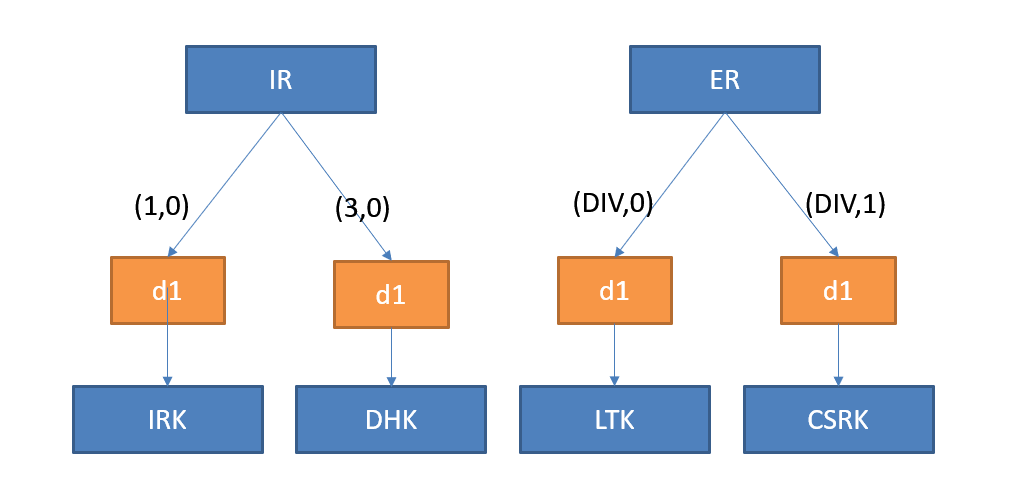
\includegraphics[width=0.85\linewidth]{./img/ble_keys} 

}

\caption{BLE 密钥层次结构}\label{fig:ch6-ble-keys}
\end{figure}

SM 涉及两个重要概念:

\begin{itemize}
\item
  \textbf{绑定}:在两个连接的设备之间交换秘密和身份信息以建立相互信赖关系。

  有的设备可能不支持绑定,因此规范定义了两种绑定模式:可绑定、不可绑定。
  建立绑定时需要使用\textbf{配对}流程交换秘密和身份信息。
\item
  \textbf{配对}:是一个用户层面的概念,需要用户输入识别码(passkey)。

  两种情况下会发生配对:1) 为了绑定;2) 用于认证未绑定的设备。
\end{itemize}

\hypertarget{ux4f7fux7528ux8bf4ux660e-6}{%
\section{使用说明}\label{ux4f7fux7528ux8bf4ux660e-6}}

\hypertarget{ux521dux59cbux5316}{%
\subsection{初始化}\label{ux521dux59cbux5316}}

\begin{enumerate}
\def\labelenumi{\arabic{enumi}.}
\item
  调用 \texttt{sm\_add\_event\_handler} 添加 SM 模块事件回调

\begin{Shaded}
\begin{Highlighting}[]
\DataTypeTok{void}\NormalTok{ sm\_add\_event\_handler}\OperatorTok{(}
  \CommentTok{// 回调函数}
\NormalTok{  btstack\_packet\_callback\_registration\_t }\OperatorTok{*}\NormalTok{ callback\_handler}\OperatorTok{);}
\end{Highlighting}
\end{Shaded}
\item
  调用 \texttt{sm\_config} 配置基础数据 ER、IR

\begin{Shaded}
\begin{Highlighting}[]
\DataTypeTok{void}\NormalTok{ sm\_config}\OperatorTok{(}
  \CommentTok{// 是否使能 SM(默认为不使能)}
  \DataTypeTok{uint8\_t}\NormalTok{ enable}\OperatorTok{,}
  \CommentTok{// 设备的 IO 能力}
\NormalTok{  io\_capability\_t io\_capability}\OperatorTok{,}
  \CommentTok{// 从角色时是否自动发送安全请求}
  \DataTypeTok{int}\NormalTok{   request\_security}\OperatorTok{,}
  \CommentTok{// 持久化数据}
  \DataTypeTok{const}\NormalTok{ sm\_persistent\_t }\OperatorTok{*}\NormalTok{persistent}\OperatorTok{);}
\end{Highlighting}
\end{Shaded}

  这里的 IO 能力 \texttt{io\_capability} 用于协商配对方法,跟设备的实际 IO 能力无关:

\begin{Shaded}
\begin{Highlighting}[]
\KeywordTok{typedef} \KeywordTok{enum} \OperatorTok{\{}
\NormalTok{  IO\_CAPABILITY\_UNINITIALIZED }\OperatorTok{=} \OperatorTok{{-}}\DecValTok{1}\OperatorTok{,}
\NormalTok{  IO\_CAPABILITY\_DISPLAY\_ONLY }\OperatorTok{=} \DecValTok{0}\OperatorTok{,}   \CommentTok{// 只支持显示}
\NormalTok{  IO\_CAPABILITY\_DISPLAY\_YES\_NO}\OperatorTok{,}     \CommentTok{// 可显示,可输入 YES、NO}
\NormalTok{  IO\_CAPABILITY\_KEYBOARD\_ONLY}\OperatorTok{,}      \CommentTok{// 只能输入}
\NormalTok{  IO\_CAPABILITY\_NO\_INPUT\_NO\_OUTPUT}\OperatorTok{,} \CommentTok{// 无输入、输出能力}
\NormalTok{  IO\_CAPABILITY\_KEYBOARD\_DISPLAY}\OperatorTok{,}   \CommentTok{// 可显示,能输入}
\OperatorTok{\}}\NormalTok{ io\_capability\_t}\OperatorTok{;}
\end{Highlighting}
\end{Shaded}

  这里的输入能力指可以输入 \(0-9\) 等 \(10\) 个数字,以及 YES、NO;显示能力是指可以显示 6 位十进制识别码(\(000000-999999\))\footnote{以及给予用户必要的提示的能力。}。

  持久化数据的定义如下:

\begin{Shaded}
\begin{Highlighting}[]
\KeywordTok{typedef} \KeywordTok{struct}\NormalTok{ sm\_persistent}
\OperatorTok{\{}
  \CommentTok{// ER 密钥}
\NormalTok{  sm\_key\_t        er}\OperatorTok{;}
  \CommentTok{// IR 密钥}
\NormalTok{  sm\_key\_t        ir}\OperatorTok{;}
  \CommentTok{// 身份地址}
\NormalTok{  bd\_addr\_t       identity\_addr}\OperatorTok{;}
  \CommentTok{// 身份地址类型(BD\_ADDR\_TYPE\_LE\_PUBLIC 或 BD\_ADDR\_TYPE\_LE\_RANDOM)}
\NormalTok{  bd\_addr\_type\_t  identity\_addr\_type}\OperatorTok{;}
\OperatorTok{\}}\NormalTok{ sm\_persistent\_t}\OperatorTok{;}
\end{Highlighting}
\end{Shaded}
\item
  通过 \texttt{sm\_set\_authentication\_requirements} 设置认证需求

\begin{Shaded}
\begin{Highlighting}[]
\DataTypeTok{void}\NormalTok{ sm\_set\_authentication\_requirements}\OperatorTok{(}
  \CommentTok{// SM\_AUTHREQ\_... 的组合:是否绑定、是否需要 MITM 保护}
  \DataTypeTok{uint8\_t}\NormalTok{ auth\_req}\OperatorTok{);}

\CommentTok{// 不可绑定}
\PreprocessorTok{\#define SM\_AUTHREQ\_NO\_BONDING       ...}
\CommentTok{// 可绑定}
\PreprocessorTok{\#define SM\_AUTHREQ\_BONDING          ...}
\CommentTok{// 使能 MITM 保护}
\PreprocessorTok{\#define SM\_AUTHREQ\_MITM\_PROTECTION  ...}
\end{Highlighting}
\end{Shaded}
\end{enumerate}

\hypertarget{ux4f7fux7528ux79c1ux6709ux968fux673aux5730ux5740}{%
\subsection{使用私有随机地址}\label{ux4f7fux7528ux79c1ux6709ux968fux673aux5730ux5740}}

如果需要使用私有随机地址,可调用 \texttt{sm\_private\_random\_address\_generation\_set\_mode} 启动 SM 模块的私有地址生成功能:

\begin{Shaded}
\begin{Highlighting}[]
\DataTypeTok{void}\NormalTok{ sm\_private\_random\_address\_generation\_set\_mode}\OperatorTok{(}
  \CommentTok{// 私有地址的生成方式}
\NormalTok{  gap\_random\_address\_type\_t random\_address\_type}\OperatorTok{);}
\end{Highlighting}
\end{Shaded}

私有地址的生成方式有三种:

\begin{Shaded}
\begin{Highlighting}[]
\KeywordTok{typedef} \KeywordTok{enum} \OperatorTok{\{}
\NormalTok{  GAP\_RANDOM\_ADDRESS\_OFF }\OperatorTok{=} \DecValTok{0}\OperatorTok{,}         \CommentTok{// 不生成(默认值)}
\NormalTok{  GAP\_RANDOM\_ADDRESS\_NON\_RESOLVABLE}\OperatorTok{,}  \CommentTok{// 生成不可解析私有地址}
\NormalTok{  GAP\_RANDOM\_ADDRESS\_RESOLVABLE}\OperatorTok{,}      \CommentTok{// 生成可解析私有地址}
\OperatorTok{\}}\NormalTok{ gap\_random\_address\_type\_t}\OperatorTok{;}
\end{Highlighting}
\end{Shaded}

启动后 SM 模块将尽快产生一个新的地址并弹出 \texttt{SM\_EVENT\_PRIVATE\_RANDOM\_ADDR\_UPDATE} 事件,
之后周期性地重新产生并弹出事件。周期默认为 15 分钟,可通过 \texttt{sm\_private\_random\_address\_generation\_set\_update\_period}
修改\footnote{没必要过于频繁地更新地址。尤其是对于可解析地址,每更新一次,就意味着泄露了一点关于 IRK 的消息。}:

\begin{Shaded}
\begin{Highlighting}[]
\DataTypeTok{void}\NormalTok{ sm\_private\_random\_address\_generation\_set\_update\_period}\OperatorTok{(}
  \DataTypeTok{int}\NormalTok{ period\_ms}\OperatorTok{);}
\end{Highlighting}
\end{Shaded}

\hypertarget{sm-ux4e8bux4ef6ux56deux8c03}{%
\subsection{SM 事件回调}\label{sm-ux4e8bux4ef6ux56deux8c03}}

SM 模块的事件回调函数将收到一系列事件,App 的主要工作就在于响应这些事件。

\begin{itemize}
\item
  \texttt{SM\_EVENT\_PRIVATE\_RANDOM\_ADDR\_UPDATE}

  SM 生成了一个新的私有随机地址。App 此时可以更新广播地址\footnote{注意:当该广播是可连接的并且正在广播时,不允许修改地址。},比如:

\begin{Shaded}
\begin{Highlighting}[]
\CommentTok{// 更新广播集 0 的随机地址}
\NormalTok{gap\_set\_adv\_set\_random\_addr}\OperatorTok{(}\DecValTok{0}\OperatorTok{,}
\NormalTok{  sm\_private\_random\_addr\_update\_get\_address}\OperatorTok{(}\NormalTok{packet}\OperatorTok{));}
\end{Highlighting}
\end{Shaded}
\end{itemize}

与地址解析、查找有关的 3 个事件:

\begin{itemize}
\item
  \texttt{SM\_EVENT\_IDENTITY\_RESOLVING\_STARTED}:开始解析某个地址

  使用以下 API 可读取正在解析的地址等信息:

  \begin{itemize}
  \tightlist
  \item
    \texttt{sm\_event\_identity\_resolving\_started\_get\_handle(packet)}:连接句柄
  \item
    \texttt{sm\_event\_identity\_resolving\_started\_get\_addr\_type(packet)}:正在解析的地址类型
  \item
    \texttt{sm\_event\_identity\_resolving\_started\_get\_address(packet,\ addr)}:正在解析的地址
  \end{itemize}
\item
  \texttt{SM\_EVENT\_IDENTITY\_RESOLVING\_FAILED}:解析失败

  使用以下 API 可读取解析失败的地址等信息:

  \begin{itemize}
  \tightlist
  \item
    \texttt{sm\_event\_identity\_resolving\_failed\_get\_handle(packet)}:连接句柄
  \item
    \texttt{sm\_event\_identity\_resolving\_failed\_get\_addr\_type(packet)}:正在解析的地址类型
  \item
    \texttt{sm\_event\_identity\_resolving\_failed\_get\_address(packet,\ addr)}:正在解析的地址
  \end{itemize}
\item
  \texttt{SM\_EVENT\_IDENTITY\_RESOLVING\_SUCCEEDED}:解析成功

  使用以下 API 可读取解析成功的地址等信息:

  \begin{itemize}
  \tightlist
  \item
    \texttt{sm\_event\_identity\_resolving\_succeeded\_get\_handle(packet)}:连接句柄
  \item
    \texttt{sm\_event\_identity\_resolving\_succeeded\_get\_addr\_type(packet)}:正在解析的地址类型
  \item
    \texttt{sm\_event\_identity\_resolving\_succeeded\_get\_address(packet,\ addr)}:正在解析的地址
  \item
    \texttt{sm\_event\_identity\_resolving\_succeeded\_get\_le\_device\_db\_index(packet)}:在``\protect\hyperlink{ch98-le-dev-db}{设备数据库}''里的序号
  \end{itemize}

  例如,通过下面的代码获取解析出的身份地址:

\begin{Shaded}
\begin{Highlighting}[]
\DataTypeTok{uint16\_t}\NormalTok{ index }\OperatorTok{=}
\NormalTok{    sm\_event\_identity\_resolving\_succeeded\_get\_le\_device\_db\_index}\OperatorTok{(}\NormalTok{packet}\OperatorTok{);}
\DataTypeTok{const}\NormalTok{ le\_device\_memory\_db\_t }\OperatorTok{*}\NormalTok{item }\OperatorTok{=}
\NormalTok{    le\_device\_db\_from\_key}\OperatorTok{(}\NormalTok{index}\OperatorTok{);}
\NormalTok{printf}\OperatorTok{(}\StringTok{"RESOLVING\_SUCCEEDED: (\%d) "}\OperatorTok{,}\NormalTok{ index}\OperatorTok{);}
\ControlFlowTok{if} \OperatorTok{(}\NormalTok{item}\OperatorTok{)}
\NormalTok{    printf\_hexdump}\OperatorTok{(}\NormalTok{item}\OperatorTok{{-}\textgreater{}}\NormalTok{addr}\OperatorTok{,}\NormalTok{ BD\_ADDR\_LEN}\OperatorTok{);}
\ControlFlowTok{else}
\NormalTok{    printf}\OperatorTok{(}\StringTok{"ERROR: should not happen"}\OperatorTok{);}
\NormalTok{printf}\OperatorTok{(}\StringTok{"}\SpecialCharTok{\textbackslash{}n}\StringTok{"}\OperatorTok{);}
\end{Highlighting}
\end{Shaded}
\end{itemize}

与配对有关的 6 个事件:

\begin{itemize}
\item
  \texttt{SM\_EVENT\_JUST\_WORKS\_REQUEST}:JUST\_WORKS 请求,等待用户接收或拒绝

  调用 \texttt{sm\_just\_works\_confirm} 接受,\texttt{sm\_bonding\_decline} 拒绝。
\item
  \texttt{SM\_EVENT\_PASSKEY\_DISPLAY\_NUMBER}:显示识别码

  App 收到此事件后显示识别码,并提示用户在对端输入此识别码。
\item
  \texttt{SM\_EVENT\_PASSKEY\_DISPLAY\_CANCEL}:不要再显示识别码

  App 收到此事件后应该刷新显示,不再呈现识别码。
\item
  \texttt{SM\_EVENT\_PASSKEY\_INPUT\_NUMBER}:提示用户输入识别码

  App 收到此事件后提示用户输入识别码,然后调用 \texttt{sm\_passkey\_input} 把用户的输入传递到协议栈。
  调用 \texttt{sm\_bonding\_decline} 可中止配对。
\end{itemize}

SM 状态改变事件:

\begin{itemize}
\item
  \texttt{SM\_EVENT\_STATE\_CHANGED}

  这个事件指示 SM 总状态的变化。使用 \texttt{decode\_hci\_event} 将其解析为 \texttt{sm\_event\_state\_changed\_t}:

\begin{Shaded}
\begin{Highlighting}[]
\KeywordTok{typedef} \KeywordTok{struct}\NormalTok{ sm\_event\_state\_changed }\OperatorTok{\{}
  \CommentTok{// 连接句柄}
  \DataTypeTok{uint16\_t}\NormalTok{ conn\_handle}\OperatorTok{;}
  \CommentTok{// 状态变化的原因}
  \DataTypeTok{uint8\_t}\NormalTok{ reason}\OperatorTok{;}
\OperatorTok{\}}\NormalTok{ sm\_event\_state\_changed\_t}\OperatorTok{;}

\DataTypeTok{const}\NormalTok{ sm\_event\_state\_changed\_t }\OperatorTok{*}\NormalTok{state\_changed }\OperatorTok{=}
\NormalTok{  decode\_hci\_event}\OperatorTok{(}\NormalTok{packet}\OperatorTok{,}\NormalTok{ sm\_event\_state\_changed\_t}\OperatorTok{);}
\end{Highlighting}
\end{Shaded}

  这里的 \texttt{reason} 即 SM 的几种\textbf{主要}状态:

\begin{Shaded}
\begin{Highlighting}[]
\KeywordTok{enum}\NormalTok{ sm\_state\_t}
\OperatorTok{\{}
\NormalTok{  SM\_STARTED}\OperatorTok{,}                 \CommentTok{// SM 启动}
\NormalTok{  SM\_FINAL\_PAIRED}\OperatorTok{,}            \CommentTok{// 已配对}
\NormalTok{  SM\_FINAL\_REESTABLISHED}\OperatorTok{,}     \CommentTok{// 已重新建立}
\NormalTok{  SM\_FINAL\_FAIL\_PROTOCOL}\OperatorTok{,}     \CommentTok{// 协议流程错误}
\NormalTok{  SM\_FINAL\_FAIL\_TIMEOUT}\OperatorTok{,}      \CommentTok{// 超时}
\NormalTok{  SM\_FINAL\_FAIL\_DISCONNECT}\OperatorTok{,}   \CommentTok{// 连接断开}
\OperatorTok{\};}
\end{Highlighting}
\end{Shaded}
\end{itemize}

\hypertarget{ux6bcfux4e2aux8fdeux63a5ux7684ux4e2aux6027ux5316ux8bbeux7f6e}{%
\subsection{每个连接的个性化设置}\label{ux6bcfux4e2aux8fdeux63a5ux7684ux4e2aux6027ux5316ux8bbeux7f6e}}

SM API 支持为每个连接进行个性化的设置:

\begin{Shaded}
\begin{Highlighting}[]
\DataTypeTok{void}\NormalTok{ sm\_config\_conn}\OperatorTok{(}
  \CommentTok{// 连接句柄}
\NormalTok{  hci\_con\_handle\_t con\_handle}\OperatorTok{,}
  \CommentTok{// IO 能力}
\NormalTok{  io\_capability\_t io\_capability}\OperatorTok{,}
  \CommentTok{// SM\_AUTHREQ\_... 的组合:是否绑定、是否需要 MITM 保护}
  \DataTypeTok{uint8\_t}\NormalTok{ auth\_req}\OperatorTok{);}
\end{Highlighting}
\end{Shaded}

注意,这个 API 只允许在 HCI 事件 \texttt{HCI\_SUBEVENT\_LE\_ENHANCED\_CONNECTION\_COMPLETE} 的回调里调用。即使 SM 为禁用状态,
也可以使用这个 API 为单个连接使能 SM。

\hypertarget{ux5730ux5740ux89e3ux6790ux67e5ux627e}{%
\subsection{地址解析、查找}\label{ux5730ux5740ux89e3ux6790ux67e5ux627e}}

通过 \texttt{sm\_address\_resolution\_lookup} 可以``手动''触发蓝牙设备地址的解析、查找:

\begin{Shaded}
\begin{Highlighting}[]
\DataTypeTok{int}\NormalTok{ sm\_address\_resolution\_lookup}\OperatorTok{(}
  \DataTypeTok{uint8\_t}\NormalTok{ addr\_type}\OperatorTok{,}  \CommentTok{// 地址类型}
\NormalTok{  bd\_addr\_t addr}\OperatorTok{);}    \CommentTok{// 地址}
\end{Highlighting}
\end{Shaded}

这里的``查找''指是的在``\protect\hyperlink{ch98-le-dev-db}{设备数据库}''中查找。如果传入的地址可解析私有地址,
那么将尝试解析该地址。

这个函数将待查地址加入一个处理队列,如果成功加入,返回值为 0;反之返回非 0 值。
解析、查找的结果通过 SM\_EVENT\_IDENTITY\_RESOLVING\_FAILED、
SM\_EVENT\_IDENTITY\_RESOLVING\_SUCCEEDED 等事件上报。

\hypertarget{ch-misc}{%
\chapter{杂项}\label{ch-misc}}

\hypertarget{ux63a5ux6536-cte}{%
\section{接收 CTE}\label{ux63a5ux6536-cte}}

共有四种 CTE 接收、发送方式\footnote{参考《Application Note: Direction Finding Solution》。}。
以 AoA 为例,各种方式的使用方法如下。

\hypertarget{ux57faux4e8eux8fdeux63a5ux7684-cte-ux63a5ux6536ux548cux53d1ux9001}{%
\subsection{基于连接的 CTE 接收和发送}\label{ux57faux4e8eux8fdeux63a5ux7684-cte-ux63a5ux6536ux548cux53d1ux9001}}

这种方式的使用可参考 SDK \emph{Central CTE} 和 \emph{Peripehral LED \& CTE}。

\hypertarget{ux53d1ux9001ux65b9}{%
\subsubsection{发送方}\label{ux53d1ux9001ux65b9}}

建立连接后:

\begin{enumerate}
\def\labelenumi{\arabic{enumi}.}
\item
  调用 \texttt{gap\_set\_connection\_cte\_tx\_param} 配置发送参数:

\begin{Shaded}
\begin{Highlighting}[]
\DataTypeTok{uint8\_t}\NormalTok{ gap\_set\_connection\_cte\_tx\_param}\OperatorTok{(}
  \CommentTok{// 连接句柄}
  \DataTypeTok{const}\NormalTok{ hci\_con\_handle\_t  conn\_handle}\OperatorTok{,}
  \CommentTok{// 允许发送的 CTE 类型组合}
  \DataTypeTok{const} \DataTypeTok{uint8\_t}\NormalTok{           cte\_types}\OperatorTok{,}
  \CommentTok{// 用于 AoD 发送的天线切换模板的长度}
  \DataTypeTok{const} \DataTypeTok{uint8\_t}\NormalTok{           switching\_pattern\_len}\OperatorTok{,}
  \CommentTok{// 用于 AoD 发送的天线切换模板}
  \DataTypeTok{const} \DataTypeTok{uint8\_t}          \OperatorTok{*}\NormalTok{antenna\_ids}
\OperatorTok{);}
\end{Highlighting}
\end{Shaded}

  对于 AoA 模式,不需要配置天线切换模板,但是模板的长度必须至少为 \(2\):

\begin{Shaded}
\begin{Highlighting}[]
\NormalTok{gap\_set\_connection\_cte\_tx\_param}\OperatorTok{(}
\NormalTok{  con\_handle}\OperatorTok{,} \OperatorTok{(}\DecValTok{1} \OperatorTok{\textless{}\textless{}}\NormalTok{ CTE\_AOA}\OperatorTok{),} \DecValTok{2}\OperatorTok{,}\NormalTok{ NULL}\OperatorTok{);}
\end{Highlighting}
\end{Shaded}
\item
  调用 \texttt{gap\_set\_connection\_cte\_response\_enable} 使能 CTE 响应:

\begin{Shaded}
\begin{Highlighting}[]
\DataTypeTok{uint8\_t}\NormalTok{ gap\_set\_connection\_cte\_response\_enable}\OperatorTok{(}
  \CommentTok{// 连接句柄}
  \DataTypeTok{const}\NormalTok{ hci\_con\_handle\_t  conn\_handle}\OperatorTok{,}
  \CommentTok{// 是否使能}
  \DataTypeTok{const} \DataTypeTok{uint8\_t}\NormalTok{           enable}\OperatorTok{);}
\end{Highlighting}
\end{Shaded}
\end{enumerate}

\hypertarget{ux63a5ux6536ux65b9}{%
\subsubsection{接收方}\label{ux63a5ux6536ux65b9}}

使用 \texttt{ll\_set\_def\_antenna} 配置默认天线。建立连接后:

\begin{enumerate}
\def\labelenumi{\arabic{enumi}.}
\item
  调用 \texttt{gap\_set\_connection\_cte\_rx\_param} 配置接收参数:

\begin{Shaded}
\begin{Highlighting}[]
\DataTypeTok{uint8\_t}\NormalTok{ gap\_set\_connection\_cte\_rx\_param}\OperatorTok{(}
  \CommentTok{// 连接句柄}
  \DataTypeTok{const}\NormalTok{ hci\_con\_handle\_t  conn\_handle}\OperatorTok{,}
  \CommentTok{// 是否使能 CTE 采样}
  \DataTypeTok{const} \DataTypeTok{uint8\_t}\NormalTok{           sampling\_enable}\OperatorTok{,}
  \CommentTok{// 时隙长度}
  \DataTypeTok{const}\NormalTok{ cte\_slot\_duration\_type\_t slot\_durations}\OperatorTok{,}
  \CommentTok{// 天线切换模板的长度}
  \DataTypeTok{const} \DataTypeTok{uint8\_t}\NormalTok{           switching\_pattern\_len}\OperatorTok{,}
  \CommentTok{// 天线切换模板}
  \DataTypeTok{const} \DataTypeTok{uint8\_t}          \OperatorTok{*}\NormalTok{antenna\_ids}\OperatorTok{);}
\end{Highlighting}
\end{Shaded}

  时隙长度共有两种:

\begin{Shaded}
\begin{Highlighting}[]
\KeywordTok{typedef} \KeywordTok{enum}
\OperatorTok{\{}
\NormalTok{    CTE\_SLOT\_DURATION\_1US }\OperatorTok{=} \DecValTok{1}\OperatorTok{,}
\NormalTok{    CTE\_SLOT\_DURATION\_2US }\OperatorTok{=} \DecValTok{2}
\OperatorTok{\}}\NormalTok{ cte\_slot\_duration\_type\_t}\OperatorTok{;}
\end{Highlighting}
\end{Shaded}

  关于天线切换模板的更多信息请参考《Application Note: Direction Finding Solution》。
\item
  调用 \texttt{gap\_set\_connection\_cte\_request\_enable} 开始发送 CTE 请求

  连接模式的 CTE 为按需发送:一方发送一次 CTE 请求,对方就响应一次。

\begin{Shaded}
\begin{Highlighting}[]
\DataTypeTok{uint8\_t}\NormalTok{ gap\_set\_connection\_cte\_request\_enable}\OperatorTok{(}
  \CommentTok{// 连接句柄}
  \DataTypeTok{const}\NormalTok{ hci\_con\_handle\_t  conn\_handle}\OperatorTok{,}
  \CommentTok{// 是否使能}
  \DataTypeTok{const} \DataTypeTok{uint8\_t}\NormalTok{           enable}\OperatorTok{,}
  \CommentTok{// 发送 CTE 请求的间隔}
  \DataTypeTok{const} \DataTypeTok{uint16\_t}\NormalTok{          requested\_cte\_interval}\OperatorTok{,}
  \CommentTok{// 请求的 CTE 的长度(范围 2\textasciitilde{}20,单位 8μs)}
  \DataTypeTok{const} \DataTypeTok{uint8\_t}\NormalTok{           requested\_cte\_length}\OperatorTok{,}
  \CommentTok{// 请求的 CTE 的类型}
  \DataTypeTok{const}\NormalTok{ cte\_type\_t        requested\_cte\_type}\OperatorTok{);}
\end{Highlighting}
\end{Shaded}

  \texttt{requested\_cte\_interval} 表示每 \texttt{requested\_cte\_interval} 个连接间隔发送一次 CTE 请求, \(0\) 表示只发送一次。
  对于 AoA,\texttt{requested\_cte\_type} 为 \texttt{CTE\_AOA}。
\item
  响应 \texttt{HCI\_SUBEVENT\_LE\_CONNECTION\_IQ\_REPORT} 事件

  使用 \texttt{decode\_hci\_le\_meta\_event} 解析事件内容:

\begin{Shaded}
\begin{Highlighting}[]
\DataTypeTok{const}\NormalTok{ le\_meta\_conn\_iq\_report\_t }\OperatorTok{*}\NormalTok{rpt }\OperatorTok{=}
\NormalTok{  decode\_hci\_le\_meta\_event}\OperatorTok{(}\NormalTok{packet}\OperatorTok{,}\NormalTok{ le\_meta\_conn\_iq\_report\_t}\OperatorTok{);}
\end{Highlighting}
\end{Shaded}

  如果 CTE 请求失败(未收到响应),则会收到 \texttt{HCI\_SUBEVENT\_LE\_CTE\_REQ\_FAILED} 事件。
\end{enumerate}

\hypertarget{misc-cte-periodic-adv}{%
\subsection{基于周期广播的 CTE 接收和发送}\label{misc-cte-periodic-adv}}

这种方式的使用可参考 SDK \emph{Periodic Advertiser} 和 \emph{Periodic Scanner}。

\hypertarget{ux53d1ux9001ux65b9-1}{%
\subsubsection{发送方}\label{ux53d1ux9001ux65b9-1}}

使能周期广播后,

\begin{enumerate}
\def\labelenumi{\arabic{enumi}.}
\item
  调用 \texttt{gap\_set\_connectionless\_cte\_tx\_param} 配置 CTE 发送参数

\begin{Shaded}
\begin{Highlighting}[]
\DataTypeTok{uint8\_t}\NormalTok{ gap\_set\_connectionless\_cte\_tx\_param}\OperatorTok{(}
  \CommentTok{// 广播句柄}
  \DataTypeTok{const} \DataTypeTok{uint8\_t}\NormalTok{       adv\_handle}\OperatorTok{,}
  \CommentTok{// CTE 长度(范围 2\textasciitilde{}20,单位 8μs)}
  \DataTypeTok{const} \DataTypeTok{uint8\_t}\NormalTok{       cte\_len}\OperatorTok{,}
  \CommentTok{// CTE 类型(对于 AoA,即 CTE\_AOA)}
  \DataTypeTok{const}\NormalTok{ cte\_type\_t    cte\_type}\OperatorTok{,}
  \CommentTok{// 一个周期广播里 CTE 发送次数}
  \DataTypeTok{const} \DataTypeTok{uint8\_t}\NormalTok{       cte\_count}\OperatorTok{,}
  \CommentTok{// 用于 AoD 发送的天线切换模板的长度}
  \DataTypeTok{const} \DataTypeTok{uint8\_t}\NormalTok{       switching\_pattern\_len}\OperatorTok{,}
  \CommentTok{// 用于 AoD 发送的天线切换模板}
  \DataTypeTok{const} \DataTypeTok{uint8\_t}      \OperatorTok{*}\NormalTok{antenna\_ids}\OperatorTok{);}
\end{Highlighting}
\end{Shaded}
\item
  调用 \texttt{gap\_set\_connectionless\_cte\_tx\_enable} 使能 CTE 发送

\begin{Shaded}
\begin{Highlighting}[]
\DataTypeTok{uint8\_t}\NormalTok{ gap\_set\_connectionless\_cte\_tx\_enable}\OperatorTok{(}
  \CommentTok{// 广播句柄}
  \DataTypeTok{const} \DataTypeTok{uint8\_t}\NormalTok{       adv\_handle}\OperatorTok{,}
  \CommentTok{// 是否使能}
  \DataTypeTok{const} \DataTypeTok{uint8\_t}\NormalTok{       cte\_enable}\OperatorTok{);}
\end{Highlighting}
\end{Shaded}

  \hypertarget{ux63a5ux6536ux65b9-1}{%
  \subsubsection{接收方}\label{ux63a5ux6536ux65b9-1}}
\end{enumerate}

与周期广播建立同步后,调用 \texttt{gap\_set\_connectionless\_iq\_sampling\_enable} 启动 CTE 接收。

\begin{Shaded}
\begin{Highlighting}[]
\DataTypeTok{uint8\_t}\NormalTok{ gap\_set\_connectionless\_iq\_sampling\_enable}\OperatorTok{(}
  \CommentTok{// 同步句柄}
  \DataTypeTok{const} \DataTypeTok{uint16\_t}\NormalTok{      sync\_handle}\OperatorTok{,}
  \CommentTok{// 是否使能采样}
  \DataTypeTok{const} \DataTypeTok{uint8\_t}\NormalTok{       sampling\_enable}\OperatorTok{,}
  \CommentTok{// 时隙长度}
  \DataTypeTok{const}\NormalTok{ cte\_slot\_duration\_type\_t slot\_durations}\OperatorTok{,}
  \CommentTok{// 每个周期广播间隔内最多接收多少个 CTE}
  \DataTypeTok{const} \DataTypeTok{uint8\_t}\NormalTok{       max\_sampled\_ctes}\OperatorTok{,}
  \CommentTok{// 天线切换模板长度}
  \DataTypeTok{const} \DataTypeTok{uint8\_t}\NormalTok{       switching\_pattern\_len}\OperatorTok{,}
  \CommentTok{// 天线切换模板}
  \DataTypeTok{const} \DataTypeTok{uint8\_t}      \OperatorTok{*}\NormalTok{antenna\_ids}\OperatorTok{);}
\end{Highlighting}
\end{Shaded}

此后就可以周期性收到 \texttt{HCI\_SUBEVENT\_LE\_CONNECTIONLESS\_IQ\_REPORT} 事件,利用 \texttt{decode\_hci\_le\_meta\_event}
解析事件内容:

\begin{Shaded}
\begin{Highlighting}[]
\DataTypeTok{const}\NormalTok{ le\_meta\_connless\_iq\_report\_t }\OperatorTok{*}\NormalTok{rpt }\OperatorTok{=}
\NormalTok{  decode\_hci\_le\_meta\_event}\OperatorTok{(}\NormalTok{packet}\OperatorTok{,}\NormalTok{ le\_meta\_connless\_iq\_report\_t}\OperatorTok{);}
\end{Highlighting}
\end{Shaded}

\hypertarget{ux57faux4e8eux79c1ux6709ux65b9ux5f0f-1-ux7684-cte-ux63a5ux6536ux548cux53d1ux9001}{%
\subsection{基于私有方式 \#1 的 CTE 接收和发送}\label{ux57faux4e8eux79c1ux6709ux65b9ux5f0f-1-ux7684-cte-ux63a5ux6536ux548cux53d1ux9001}}

这种方式最为灵活,需要配置的参数也最多,可参考 SDK \emph{Ext. Raw Packet Tx/Rx}。

\hypertarget{ux57faux4e8eux79c1ux6709ux65b9ux5f0f-2-ux7684-cte-ux63a5ux6536ux548cux53d1ux9001}{%
\subsection{基于私有方式 \#2 的 CTE 接收和发送}\label{ux57faux4e8eux79c1ux6709ux65b9ux5f0f-2-ux7684-cte-ux63a5ux6536ux548cux53d1ux9001}}

这种方式的使用可参考 SDK \emph{Central CTE} 和 \emph{Peripehral LED \& CTE}。

\hypertarget{ux53d1ux9001ux65b9-2}{%
\subsubsection{发送方}\label{ux53d1ux9001ux65b9-2}}

配置一个扩展广播集,属性设置为不可连接、不可扫描。待广播集使能后,调用 \texttt{ll\_attach\_cte\_to\_adv\_set}\footnote{参考《Controller API Reference》。}
为扩展广播附加 CTE。

\hypertarget{ux63a5ux6536ux65b9-2}{%
\subsubsection{接收方}\label{ux63a5ux6536ux65b9-2}}

启动扫描之后,调用 \texttt{ll\_scanner\_enable\_iq\_sampling}\footnote{参考《Controller API Reference》。} 使能 CTE 采样。
之后,通过 \texttt{HCI\_SUBEVENT\_LE\_VENDOR\_PRO\_CONNECTIONLESS\_IQ\_REPORT} 事件获得 CTE 报告。

\hypertarget{ux52a0ux5bc6ux4e0eux89e3ux5bc6}{%
\section{加密与解密}\label{ux52a0ux5bc6ux4e0eux89e3ux5bc6}}

\hypertarget{aes-128-ux52a0ux5bc6}{%
\subsection{AES-128 加密}\label{aes-128-ux52a0ux5bc6}}

通过 \texttt{gap\_aes\_encrypt} 进行 AES-128 加密:

\begin{Shaded}
\begin{Highlighting}[]
\DataTypeTok{uint8\_t}\NormalTok{ gap\_aes\_encrypt}\OperatorTok{(}
  \DataTypeTok{const} \DataTypeTok{uint8\_t} \OperatorTok{*}\NormalTok{key}\OperatorTok{,}           \CommentTok{// 密钥(大端模式)}
  \DataTypeTok{const} \DataTypeTok{uint8\_t} \OperatorTok{*}\NormalTok{plaintext}\OperatorTok{,}     \CommentTok{// 明文(大端模式)}
\NormalTok{  gap\_hci\_cmd\_complete\_cb\_t cb}\OperatorTok{,} \CommentTok{// 加密完成后的回调}
  \DataTypeTok{void} \OperatorTok{*}\NormalTok{user\_data}\OperatorTok{);}             \CommentTok{// 回调函数的用户数据}
\end{Highlighting}
\end{Shaded}

以 \href{https://www.nist.gov/publications/advanced-encryption-standard-aes}{FIPS 197}
里的数据为例:

\begin{verbatim}
PLAINTEXT: 00112233445566778899aabbccddeeff
KEY:       000102030405060708090a0b0c0d0e0f
CIPHERTEXT:69c4e0d86a7b0430d8cdb78070b4c55a
\end{verbatim}

写成大端模式的数组形式:

\begin{Shaded}
\begin{Highlighting}[]
\DataTypeTok{static} \DataTypeTok{const} \DataTypeTok{uint8\_t}\NormalTok{ plain\_text}\OperatorTok{[]} \OperatorTok{=}
    \OperatorTok{\{}\BaseNTok{0x00}\OperatorTok{,} \BaseNTok{0x11}\OperatorTok{,} \BaseNTok{0x22}\OperatorTok{,} \BaseNTok{0x33}\OperatorTok{,} \BaseNTok{0x44}\OperatorTok{,} \BaseNTok{0x55}\OperatorTok{,} \BaseNTok{0x66}\OperatorTok{,} \BaseNTok{0x77}\OperatorTok{,}
     \BaseNTok{0x88}\OperatorTok{,} \BaseNTok{0x99}\OperatorTok{,} \BaseNTok{0xaa}\OperatorTok{,} \BaseNTok{0xbb}\OperatorTok{,} \BaseNTok{0xcc}\OperatorTok{,} \BaseNTok{0xdd}\OperatorTok{,} \BaseNTok{0xee}\OperatorTok{,} \BaseNTok{0xff}\OperatorTok{\};}
\DataTypeTok{static} \DataTypeTok{const} \DataTypeTok{uint8\_t}\NormalTok{ key}\OperatorTok{[]} \OperatorTok{=}
    \OperatorTok{\{}\BaseNTok{0x00}\OperatorTok{,} \BaseNTok{0x01}\OperatorTok{,} \BaseNTok{0x02}\OperatorTok{,} \BaseNTok{0x03}\OperatorTok{,} \BaseNTok{0x04}\OperatorTok{,} \BaseNTok{0x05}\OperatorTok{,} \BaseNTok{0x06}\OperatorTok{,} \BaseNTok{0x07}\OperatorTok{,}
     \BaseNTok{0x08}\OperatorTok{,} \BaseNTok{0x09}\OperatorTok{,} \BaseNTok{0x0a}\OperatorTok{,} \BaseNTok{0x0b}\OperatorTok{,} \BaseNTok{0x0c}\OperatorTok{,} \BaseNTok{0x0d}\OperatorTok{,} \BaseNTok{0x0e}\OperatorTok{,} \BaseNTok{0x0f}\OperatorTok{\};}
\DataTypeTok{static} \DataTypeTok{const} \DataTypeTok{uint8\_t}\NormalTok{ cipher\_text}\OperatorTok{[]} \OperatorTok{=}
    \OperatorTok{\{}\BaseNTok{0x69}\OperatorTok{,} \BaseNTok{0xc4}\OperatorTok{,} \BaseNTok{0xe0}\OperatorTok{,} \BaseNTok{0xd8}\OperatorTok{,} \BaseNTok{0x6a}\OperatorTok{,} \BaseNTok{0x7b}\OperatorTok{,} \BaseNTok{0x04}\OperatorTok{,} \BaseNTok{0x30}\OperatorTok{,}
     \BaseNTok{0xd8}\OperatorTok{,} \BaseNTok{0xcd}\OperatorTok{,} \BaseNTok{0xb7}\OperatorTok{,} \BaseNTok{0x80}\OperatorTok{,} \BaseNTok{0x70}\OperatorTok{,} \BaseNTok{0xb4}\OperatorTok{,} \BaseNTok{0xc5}\OperatorTok{,} \BaseNTok{0x5a}\OperatorTok{\};}
\end{Highlighting}
\end{Shaded}

加密:

\begin{Shaded}
\begin{Highlighting}[]
\NormalTok{gap\_aes\_encrypt}\OperatorTok{(}\NormalTok{key}\OperatorTok{,}\NormalTok{ plain\_text}\OperatorTok{,}\NormalTok{ aes\_cb}\OperatorTok{,}\NormalTok{ NULL}\OperatorTok{);}
\end{Highlighting}
\end{Shaded}

在回调函数 \texttt{aes\_cb} 对比密文如下:

\begin{Shaded}
\begin{Highlighting}[]
\DataTypeTok{void}\NormalTok{ aes\_cb}\OperatorTok{(}\DataTypeTok{const} \DataTypeTok{uint8\_t} \OperatorTok{*}\NormalTok{return\_param}\OperatorTok{,} \DataTypeTok{const} \DataTypeTok{uint8\_t} \OperatorTok{*}\NormalTok{user\_data}\OperatorTok{)}
\OperatorTok{\{}
    \DataTypeTok{uint8\_t}\NormalTok{ reversed}\OperatorTok{[}\DecValTok{16}\OperatorTok{];}
\NormalTok{    reverse\_bytes}\OperatorTok{(}\NormalTok{return\_param }\OperatorTok{+} \DecValTok{1}\OperatorTok{,}\NormalTok{ reversed}\OperatorTok{,} \KeywordTok{sizeof}\OperatorTok{(}\NormalTok{reversed}\OperatorTok{));}
\NormalTok{    printf}\OperatorTok{(}\StringTok{"Matched: \%d}\SpecialCharTok{\textbackslash{}n}\StringTok{"}\OperatorTok{,}
\NormalTok{      memcmp}\OperatorTok{(}\NormalTok{reversed}\OperatorTok{,}\NormalTok{ cipher\_text}\OperatorTok{,} \KeywordTok{sizeof}\OperatorTok{(}\NormalTok{cipher\_text}\OperatorTok{))} \OperatorTok{==} \DecValTok{0}\OperatorTok{);}
\OperatorTok{\}}
\end{Highlighting}
\end{Shaded}

这里 \texttt{return\_param} 的内容与规范中相应 HCI 命令的 Return Parameters 一致。密文采用小端模式,
所以需要反转为大端模式,再与测试数据比较。

在上一次 AES 加密完成前,允许再次调用 \texttt{gap\_aes\_encrypt}。所有的加密任务保存在一个队列中,顺序完成。

也通过 \texttt{ll\_aes\_encrypt} 进行 AES-128 加密。
使用时务必检查返回值,若不为 0 表示硬件正忙。遇到此情况时可稍后重试。

\begin{Shaded}
\begin{Highlighting}[]
\DataTypeTok{int}\NormalTok{ ll\_aes\_encrypt}\OperatorTok{(}
  \DataTypeTok{const} \DataTypeTok{uint8\_t} \OperatorTok{*}\NormalTok{key}\OperatorTok{,}       \CommentTok{// 密钥(小端模式)}
  \DataTypeTok{const} \DataTypeTok{uint8\_t} \OperatorTok{*}\NormalTok{plaintext}\OperatorTok{,} \CommentTok{// 明文(小端模式)}
  \DataTypeTok{uint8\_t} \OperatorTok{*}\NormalTok{ciphertext}\OperatorTok{);}     \CommentTok{// 密文(大端模式)}
\end{Highlighting}
\end{Shaded}

\texttt{ll\_aes\_encrypt} 与 \texttt{gap\_aes\_encrypt} 的不同点:

\begin{itemize}
\tightlist
\item
  \texttt{ll\_aes\_encrypt} 以阻塞模式工作,不支持队列方式
\item
  \texttt{ll\_aes\_encrypt} 可以更快完成加密
\item
  数据的大小端
\end{itemize}

\hypertarget{aes-ccm}{%
\subsection{AES-CCM}\label{aes-ccm}}

CCM 是 Cipher Block Chaining-Message Authentication Code (CBC-MAC) 和 Counter 模式(CTR)的组合,同时对数据加密和生成认证信息。
通过 \texttt{gap\_start\_ccm} 启动 AES-CCM 计算\footnote{为防止与 Media Access Controller 混淆,蓝牙规范使用 MIC 代替 MAC。}:

\begin{Shaded}
\begin{Highlighting}[]
\DataTypeTok{uint8\_t}\NormalTok{ gap\_start\_ccm}\OperatorTok{(}
        \DataTypeTok{uint8\_t}\NormalTok{  type}\OperatorTok{,}        \CommentTok{// 类型:0 为加密,1 为解密}
        \DataTypeTok{uint8\_t}\NormalTok{  mic\_size}\OperatorTok{,}    \CommentTok{// MIC 长度(4 或 8 字节)}
        \DataTypeTok{uint16\_t}\NormalTok{ msg\_len}\OperatorTok{,}     \CommentTok{// 消息长度(最长 384 字节)}
        \DataTypeTok{uint16\_t}\NormalTok{ aad\_len}\OperatorTok{,}     \CommentTok{// AAD 长度(最长 16 字节,可为 0)}
        \DataTypeTok{uint32\_t}\NormalTok{ tag}\OperatorTok{,}         \CommentTok{// 数据标签(任意值)}
        \DataTypeTok{const} \DataTypeTok{uint8\_t} \OperatorTok{*}\NormalTok{key}\OperatorTok{,}   \CommentTok{// 密钥}
        \DataTypeTok{const} \DataTypeTok{uint8\_t} \OperatorTok{*}\NormalTok{nonce}\OperatorTok{,} \CommentTok{// Nonce(长度 13 字节)}
        \DataTypeTok{const} \DataTypeTok{uint8\_t} \OperatorTok{*}\NormalTok{msg}\OperatorTok{,}   \CommentTok{// 消息}
        \DataTypeTok{const} \DataTypeTok{uint8\_t} \OperatorTok{*}\NormalTok{aad}\OperatorTok{,}   \CommentTok{// AAD}
        \DataTypeTok{uint8\_t} \OperatorTok{*}\NormalTok{out\_msg}\OperatorTok{,}     \CommentTok{// 加解密输出}
\NormalTok{        gap\_hci\_cmd\_complete\_cb\_t cb}\OperatorTok{,} \CommentTok{// 计算完成后的回调}
        \DataTypeTok{void} \OperatorTok{*}\NormalTok{user\_data}\OperatorTok{);}             \CommentTok{// 回调函数的用户数据}
\end{Highlighting}
\end{Shaded}

AAD 为补充认证证数据(Additional Authenticated Data),可为数据提供额外的完整性保护。
这个函数使用了自定义的 HCI 消息 \texttt{HCI\_VENDOR\_CCM}。由于消息数据量大,这条消息仅传递指针,
因此所有的数据(\texttt{key}、\texttt{nonce}、\texttt{aad}、\texttt{msg}、\texttt{out\_msg})必须一直存在,直到计算完成方可释放。
加密时,输出到 \texttt{out\_msg} 的数据长度为 (\texttt{msg\_len} + \texttt{mic\_size});解密时,\texttt{msg} 传入的数据长度为
(\texttt{msg\_len} + \texttt{mic\_size})。

回调函数收到的 \texttt{return\_param} 参数转换自 \texttt{event\_vendor\_ccm\_complete\_t\ *}。

例如:

\begin{Shaded}
\begin{Highlighting}[]
\DataTypeTok{static} \DataTypeTok{const} \DataTypeTok{uint8\_t}\NormalTok{ plain\_text}\OperatorTok{[]} \OperatorTok{=}
    \OperatorTok{\{}\BaseNTok{0x00}\OperatorTok{,} \BaseNTok{0x11}\OperatorTok{,} \BaseNTok{0x22}\OperatorTok{,} \BaseNTok{0x33}\OperatorTok{,} \BaseNTok{0x44}\OperatorTok{,} \BaseNTok{0x55}\OperatorTok{,} \BaseNTok{0x66}\OperatorTok{,} \BaseNTok{0x77}\OperatorTok{,}
     \BaseNTok{0x88}\OperatorTok{,} \BaseNTok{0x99}\OperatorTok{,} \BaseNTok{0xaa}\OperatorTok{,} \BaseNTok{0xbb}\OperatorTok{,} \BaseNTok{0xcc}\OperatorTok{,} \BaseNTok{0xdd}\OperatorTok{,} \BaseNTok{0xee}\OperatorTok{,} \BaseNTok{0xff}\OperatorTok{\};}
\DataTypeTok{static} \DataTypeTok{const} \DataTypeTok{uint8\_t}\NormalTok{ key}\OperatorTok{[]} \OperatorTok{=}
    \OperatorTok{\{}\BaseNTok{0x00}\OperatorTok{,} \BaseNTok{0x01}\OperatorTok{,} \BaseNTok{0x02}\OperatorTok{,} \BaseNTok{0x03}\OperatorTok{,} \BaseNTok{0x04}\OperatorTok{,} \BaseNTok{0x05}\OperatorTok{,} \BaseNTok{0x06}\OperatorTok{,} \BaseNTok{0x07}\OperatorTok{,}
     \BaseNTok{0x08}\OperatorTok{,} \BaseNTok{0x09}\OperatorTok{,} \BaseNTok{0x0a}\OperatorTok{,} \BaseNTok{0x0b}\OperatorTok{,} \BaseNTok{0x0c}\OperatorTok{,} \BaseNTok{0x0d}\OperatorTok{,} \BaseNTok{0x0e}\OperatorTok{,} \BaseNTok{0x0f}\OperatorTok{\};}

\PreprocessorTok{\#define MSG\_LEN     16}
\PreprocessorTok{\#define MIC\_SIZE    4}

\DataTypeTok{static} \DataTypeTok{const} \DataTypeTok{uint8\_t}\NormalTok{ nonce}\OperatorTok{[}\DecValTok{13}\OperatorTok{]} \OperatorTok{=} \OperatorTok{\{}\DecValTok{1}\OperatorTok{\};}
\DataTypeTok{static} \DataTypeTok{uint8\_t}\NormalTok{ ccm\_enc\_out}\OperatorTok{[}\NormalTok{MSG\_LEN }\OperatorTok{+}\NormalTok{ MIC\_SIZE}\OperatorTok{];}
\DataTypeTok{static} \DataTypeTok{uint8\_t}\NormalTok{ ccm\_dec\_out}\OperatorTok{[}\NormalTok{MSG\_LEN}\OperatorTok{];}
\end{Highlighting}
\end{Shaded}

加密:

\begin{Shaded}
\begin{Highlighting}[]
\NormalTok{gap\_start\_ccm}\OperatorTok{(}\DecValTok{0}\OperatorTok{,}\NormalTok{ MIC\_SIZE}\OperatorTok{,}\NormalTok{ MSG\_LEN}\OperatorTok{,} \DecValTok{0}\OperatorTok{,} \DecValTok{0}\OperatorTok{,}
\NormalTok{            key}\OperatorTok{,}\NormalTok{ nonce}\OperatorTok{,}\NormalTok{ plain\_text}\OperatorTok{,}\NormalTok{ NULL}\OperatorTok{,}
\NormalTok{            ccm\_enc\_out}\OperatorTok{,}\NormalTok{ ccm\_enc\_cb}\OperatorTok{,}\NormalTok{ NULL}\OperatorTok{);;}
\end{Highlighting}
\end{Shaded}

在回调函数 \texttt{ccm\_enc\_cb} 里解密:

\begin{Shaded}
\begin{Highlighting}[]
\DataTypeTok{void}\NormalTok{ ccm\_enc\_cb}\OperatorTok{(}\DataTypeTok{const} \DataTypeTok{uint8\_t} \OperatorTok{*}\NormalTok{return\_param}\OperatorTok{,} \DataTypeTok{const} \DataTypeTok{uint8\_t} \OperatorTok{*}\NormalTok{user\_data}\OperatorTok{)}
\OperatorTok{\{}
  \DataTypeTok{const}\NormalTok{ event\_vendor\_ccm\_complete\_t }\OperatorTok{*}\NormalTok{complete }\OperatorTok{=}
    \OperatorTok{(}\DataTypeTok{const}\NormalTok{ event\_vendor\_ccm\_complete\_t }\OperatorTok{*)}\NormalTok{return\_param}\OperatorTok{;}
\NormalTok{  gap\_start\_ccm}\OperatorTok{(}\DecValTok{1}\OperatorTok{,}\NormalTok{ MIC\_SIZE}\OperatorTok{,}\NormalTok{ MSG\_LEN}\OperatorTok{,} \DecValTok{0}\OperatorTok{,} \DecValTok{0}\OperatorTok{,}
\NormalTok{        key}\OperatorTok{,}\NormalTok{ nonce}\OperatorTok{,}\NormalTok{ ccm\_enc\_out}\OperatorTok{,}\NormalTok{ NULL}\OperatorTok{,}
\NormalTok{        ccm\_dec\_out}\OperatorTok{,}\NormalTok{ ccm\_dec\_cb}\OperatorTok{,}\NormalTok{ NULL}\OperatorTok{);}
\OperatorTok{\}}
\end{Highlighting}
\end{Shaded}

在回调函数 \texttt{ccm\_dec\_cb} 里检查 MIC 验证状态并比对数据:

\begin{Shaded}
\begin{Highlighting}[]
\DataTypeTok{void}\NormalTok{ ccm\_dec\_cb}\OperatorTok{(}\DataTypeTok{const} \DataTypeTok{uint8\_t} \OperatorTok{*}\NormalTok{return\_param}\OperatorTok{,} \DataTypeTok{void} \OperatorTok{*}\NormalTok{user\_data}\OperatorTok{)}
\OperatorTok{\{}
  \DataTypeTok{const}\NormalTok{ event\_vendor\_ccm\_complete\_t }\OperatorTok{*}\NormalTok{complete }\OperatorTok{=}
    \OperatorTok{(}\DataTypeTok{const}\NormalTok{ event\_vendor\_ccm\_complete\_t }\OperatorTok{*)}\NormalTok{return\_param}\OperatorTok{;}
\NormalTok{  printf}\OperatorTok{(}\StringTok{"CCM DEC Status: \%d}\SpecialCharTok{\textbackslash{}n}\StringTok{"}\OperatorTok{,}\NormalTok{ complete}\OperatorTok{{-}\textgreater{}}\NormalTok{status}\OperatorTok{);}
\NormalTok{  printf}\OperatorTok{(}\StringTok{"Matched: \%d}\SpecialCharTok{\textbackslash{}n}\StringTok{"}\OperatorTok{,}
\NormalTok{    memcmp}\OperatorTok{(}\NormalTok{ccm\_dec\_out}\OperatorTok{,}\NormalTok{ plain\_text}\OperatorTok{,} \KeywordTok{sizeof}\OperatorTok{(}\NormalTok{plain\_text}\OperatorTok{))} \OperatorTok{==} \DecValTok{0}\OperatorTok{);}
\OperatorTok{\}}
\end{Highlighting}
\end{Shaded}

\texttt{event\_vendor\_ccm\_complete\_t} 的定义如下:

\begin{Shaded}
\begin{Highlighting}[]
\KeywordTok{typedef} \KeywordTok{struct}
\OperatorTok{\{}
    \DataTypeTok{uint8\_t}\NormalTok{  status}\OperatorTok{;}   \CommentTok{// 状态码}
    \DataTypeTok{uint8\_t}\NormalTok{  type}\OperatorTok{;}
    \DataTypeTok{uint8\_t}\NormalTok{  mic\_size}\OperatorTok{;}
    \DataTypeTok{uint16\_t}\NormalTok{ msg\_len}\OperatorTok{;}
    \DataTypeTok{uint16\_t}\NormalTok{ aad\_len}\OperatorTok{;}
    \DataTypeTok{uint32\_t}\NormalTok{ tag}\OperatorTok{;}
    \DataTypeTok{uint8\_t} \OperatorTok{*}\NormalTok{out\_msg}\OperatorTok{;}
\OperatorTok{\}}\NormalTok{ event\_vendor\_ccm\_complete\_t}\OperatorTok{;}
\end{Highlighting}
\end{Shaded}

状态码在加密时,总是为 0;在解密时,0 表示 MIC 验证通过,非 0 表示失败。其它域与传入
\texttt{gap\_start\_ccm} 的参数一一对应、相等。

在上一次 AES-CCM 计算完成前,允许再次调用 \texttt{gap\_start\_ccm}。所有的计算任务保存在一个队列中,顺序完成。

\hypertarget{ux517cux5bb9ux6027}{%
\section{兼容性}\label{ux517cux5bb9ux6027}}

\hypertarget{data-length-ux4e0e-mtu}{%
\subsection{Data Length 与 MTU}\label{data-length-ux4e0e-mtu}}

低功耗蓝牙进入连接模式后,各层分别协商通信中数据包的大小,对于 ATT 层,由 MTU EXCHANGE 流程实现;对于链路层,由 DATA LENGTH 更新流程实现。

按照规范,进入连接模式后,DATA LENGTH 更新流程可以由主或从设备在任何时刻发起。这导致了一个问题:某些芯片无法处理对方设备``随时''发起的
DATA LENGTH 更新流程\footnote{\url{https://ingchips.github.io/blog/2021-06-02-sdk-6/\#\%E5\%85\%BC\%E5\%AE\%B9\%E6\%80\%A7}}。
为了更新地兼容不同的芯片,协议栈定义了两个配置项:

\begin{Shaded}
\begin{Highlighting}[]
\KeywordTok{enum}\NormalTok{ btstack\_config\_item }\OperatorTok{\{}
\NormalTok{    STACK\_ATT\_SERVER\_ENABLE\_AUTO\_DATA\_LEN\_REQ }\OperatorTok{=} \DecValTok{1}\OperatorTok{,}
\NormalTok{    STACK\_GATT\_CLIENT\_DISABLE\_AUTO\_DATA\_LEN\_REQ }\OperatorTok{=} \DecValTok{2}\OperatorTok{,}
    \CommentTok{//...}
\OperatorTok{\};}
\end{Highlighting}
\end{Shaded}

这两个配置分别控制 GATT Server、Client 在 MTU EXCHANGE 时是否自动发起 DATA LENGTH 更新流程。默认情况下,Servier 不会自动发起更新流程,
而 Client 会自动发起。

通过 \texttt{btstack\_config} 配置:

\begin{Shaded}
\begin{Highlighting}[]
\DataTypeTok{void}\NormalTok{ btstack\_config}\OperatorTok{(}
  \CommentTok{// btstack\_config\_item 的比特组合}
  \DataTypeTok{uint32\_t}\NormalTok{ flags}\OperatorTok{);}
\end{Highlighting}
\end{Shaded}

\hypertarget{api-ux8fd4ux56deux503c}{%
\section{API 返回值}\label{api-ux8fd4ux56deux503c}}

绝大多数协议栈 API 都带有 \texttt{uint8\_t} 型的返回值,\(0\) 为成功,非 \(0\) 为错误。开发者需要关注这些返回值。

几个例子:

\begin{itemize}
\item
  \texttt{att\_server\_notify} 的返回值:

  \begin{itemize}
  \tightlist
  \item
    \(0\):成功
  \item
    \texttt{BTSTACK\_LE\_CHANNEL\_NOT\_EXIST}:连接不存在(连接句柄参数错误?)
  \item
    \texttt{BTSTACK\_ACL\_BUFFERS\_FULL}:内存已满
  \end{itemize}
\item
  \texttt{gap\_set\_ext\_adv\_para} 的返回值:

  \begin{itemize}
  \tightlist
  \item
    \(0\):成功
  \item
    \texttt{BTSTACK\_MEMORY\_ALLOC\_FAILED}:内存已满
  \end{itemize}
\end{itemize}

\hypertarget{ux952eux503cux5b58ux50a8}{%
\section{键值存储}\label{ux952eux503cux5b58ux50a8}}

协议包含了一个简单的键值存储模块(\emph{kv\_storage}),其键(\emph{key}) 为 \texttt{uint8\_t},值(\emph{value}) 为长度不超过 \texttt{KV\_VALUE\_MAX\_LEN}
的数组。

开发者可以在 App 里使用这个模块,\emph{key} 的取值范围应该在 \texttt{KV\_USER\_KEY\_START} 和 \texttt{KV\_USER\_KEY\_END} 之间。需要注意以下几点:

\begin{enumerate}
\def\labelenumi{\arabic{enumi}.}
\tightlist
\item
  该模块查找一个 \emph{key} 的时间复杂度为 \(\mathcal{O}(n)\);
\item
  该模块不是线程安全的。
\end{enumerate}

这个模块本身没有数据持久化。持久化需要开发者通过 \texttt{kv\_init}\footnote{只能在 \texttt{app\_main} 就调用。} 提供回调来实现:

\begin{Shaded}
\begin{Highlighting}[]
\DataTypeTok{void}\NormalTok{ kv\_init}\OperatorTok{(}
  \CommentTok{// 用来保存数据的回调}
\NormalTok{  f\_kv\_write\_to\_nvm f\_write}\OperatorTok{,}
  \CommentTok{// 用来读取(恢复)数据的回调}
\NormalTok{  f\_kv\_read\_from\_nvm f\_read}\OperatorTok{);}
\end{Highlighting}
\end{Shaded}

当键值存储模块初始化时,会调用 \texttt{f\_read} 恢复之前的数据状态;当存储里的数据更新后,键值存储模块会自动调用 \texttt{f\_write} 回调。
考虑到 Flash 不宜频繁擦写,键值存储模块通过定时器超时来触发写入。每当数据更新时,复位定时器。整个储存的总大小为
\texttt{DB\_CAPACITY\_SIZE}。

这个存储模块的增、删、改、查等接口如下。

\begin{itemize}
\item
  增/改:\texttt{kv\_put}

\begin{Shaded}
\begin{Highlighting}[]
\CommentTok{// 如果 key 不存在,为“增”;如果 key 存在,为“改”}
\DataTypeTok{int}\NormalTok{ kv\_put}\OperatorTok{(}
  \DataTypeTok{const}\NormalTok{ kvkey\_t key}\OperatorTok{,}
  \CommentTok{// 值}
  \DataTypeTok{const} \DataTypeTok{uint8\_t} \OperatorTok{*}\NormalTok{data}\OperatorTok{,}
  \CommentTok{// 值的长度}
  \DataTypeTok{int16\_t}\NormalTok{ len}\OperatorTok{);}
\end{Highlighting}
\end{Shaded}
\item
  删:\texttt{kv\_remove}

\begin{Shaded}
\begin{Highlighting}[]
\DataTypeTok{void}\NormalTok{ kv\_remove}\OperatorTok{(}
  \CommentTok{// 键}
  \DataTypeTok{const}\NormalTok{ kvkey\_t key}\OperatorTok{)}
\end{Highlighting}
\end{Shaded}
\item
  查:\texttt{kv\_get}

\begin{Shaded}
\begin{Highlighting}[]
\CommentTok{// 返回:指向值的指针}
\DataTypeTok{uint8\_t} \OperatorTok{*}\NormalTok{kv\_get}\OperatorTok{(}
  \CommentTok{// 键}
  \DataTypeTok{const}\NormalTok{ kvkey\_t key}\OperatorTok{,}
  \CommentTok{// 输出:值的长度}
  \DataTypeTok{int16\_t} \OperatorTok{*}\NormalTok{len}\OperatorTok{);}
\end{Highlighting}
\end{Shaded}

  这个 API 返回的指针直接指向模块内值的存储空间,允许开发者在不改变值的长度的前提下修改其的内容。
  修改之后需要调用 \texttt{kv\_value\_modified} 告知存储模块。
\item
  遍历:\texttt{kv\_visit}

\begin{Shaded}
\begin{Highlighting}[]
\DataTypeTok{void}\NormalTok{ kv\_visit}\OperatorTok{(}
  \CommentTok{// 访问者回调}
\NormalTok{  f\_kv\_visitor visitor}\OperatorTok{,}
  \CommentTok{// 传递给回调的用户参数}
  \DataTypeTok{void} \OperatorTok{*}\NormalTok{user\_data}\OperatorTok{);}
\end{Highlighting}
\end{Shaded}

  使用这个 API 可以遍历存储内所有的键值对。
\end{itemize}

\hypertarget{ch98-le-dev-db}{%
\section{设备数据库}\label{ch98-le-dev-db}}

设备数据库模块(\emph{le\_device\_db})负责存储、管理设备的绑定信息。这个模块是基于键值存储模块实现的,
所能存储的设备个数等于软件包所支持的连接数目。删、查等接口如下。

\begin{itemize}
\item
  查:\texttt{le\_device\_db\_find}

\begin{Shaded}
\begin{Highlighting}[]
\NormalTok{le\_device\_memory\_db\_t }\OperatorTok{*}\NormalTok{le\_device\_db\_find}\OperatorTok{(}
  \CommentTok{// 待查设备的地址类型}
  \DataTypeTok{const} \DataTypeTok{int}\NormalTok{ addr\_type}\OperatorTok{,}
  \CommentTok{// 待查设备的地址}
  \DataTypeTok{const}\NormalTok{ bd\_addr\_t addr}\OperatorTok{,}
  \CommentTok{// 输出:在数据库里的序号}
  \DataTypeTok{int} \OperatorTok{*}\NormalTok{index}\OperatorTok{);}
\end{Highlighting}
\end{Shaded}
\item
  删

  直接按地址删除:

\begin{Shaded}
\begin{Highlighting}[]
\DataTypeTok{void}\NormalTok{ le\_device\_db\_remove}\OperatorTok{(}
  \CommentTok{// 待删设备的地址类型}
  \DataTypeTok{const} \DataTypeTok{int}\NormalTok{ addr\_type}\OperatorTok{,}
  \CommentTok{// 待删设备的地址}
  \DataTypeTok{const}\NormalTok{ bd\_addr\_t addr}\OperatorTok{);}
\end{Highlighting}
\end{Shaded}

  根据在数据库里的编号删除:

\begin{Shaded}
\begin{Highlighting}[]
\DataTypeTok{void}\NormalTok{ le\_device\_db\_remove\_key}\OperatorTok{(}
  \CommentTok{// 待删设备在数据库里的编号}
  \DataTypeTok{int}\NormalTok{ index}\OperatorTok{);}
\end{Highlighting}
\end{Shaded}
\item
  遍历

  这个模块支持迭代器遍历:

\begin{Shaded}
\begin{Highlighting}[]
\NormalTok{le\_device\_memory\_db\_iter\_t iter}\OperatorTok{;}
\NormalTok{le\_device\_db\_iter\_init}\OperatorTok{(\&}\NormalTok{iter}\OperatorTok{);}
\ControlFlowTok{while} \OperatorTok{(}\NormalTok{le\_device\_db\_iter\_next}\OperatorTok{(\&}\NormalTok{iter}\OperatorTok{))}
\OperatorTok{\{}
\NormalTok{    le\_device\_memory\_db\_t }\OperatorTok{*}\NormalTok{cur }\OperatorTok{=}\NormalTok{ le\_device\_db\_iter\_cur}\OperatorTok{(\&}\NormalTok{iter}\OperatorTok{);}
    \CommentTok{// ...}
\OperatorTok{\}}
\end{Highlighting}
\end{Shaded}
\end{itemize}

\hypertarget{ch-misc-synced-api}{%
\section{同步版 API}\label{ch-misc-synced-api}}

SDK 提供的工具模块 \emph{btstack\_sync} 里包含几个 GAP、GATT 客户端同步版本的 API。
要使用这些 API 必须先初始化同步执行器。

\begin{itemize}
\item
  v8.2 及以上版本(基于 \texttt{btstack\_push\_user\_runnable} 实现)

  如下创建同步执行器对象:

\begin{Shaded}
\begin{Highlighting}[]
\KeywordTok{struct}\NormalTok{ gatt\_client\_synced\_runner }\OperatorTok{*}\NormalTok{synced\_runner }\OperatorTok{=}
\NormalTok{    gatt\_client\_create\_sync\_runner}\OperatorTok{(}\NormalTok{enable\_gap\_api}\OperatorTok{);}
\end{Highlighting}
\end{Shaded}

  这里的 \texttt{enable\_gap\_api} 表示是否使能 GAP 同步版 API。
\item
  v8.2 以下版本(基于 \texttt{btstack\_push\_user\_msg} 实现)

  \begin{rmdcaution}
    v8.2 以下版本的 \emph{gatt\_client\_util} 模块仅提供 GATT 客户端同步版本
    API, 未提供 GAP 同步版 API ------ 开发者可参考 v8.2 自行添加。
    \end{rmdcaution}

  \begin{enumerate}
  \def\labelenumi{\arabic{enumi}.}
  \item
    基于 \texttt{btstack\_push\_user\_msg} 实现一个消息传递函数,

\begin{Shaded}
\begin{Highlighting}[]
\CommentTok{// runner 为同步执行器}
\CommentTok{// msg\_id 为同步执行器内部的消息,从其数据类型可看出最多只有 256 种 ID,}
\CommentTok{// 可以映射到 btstack\_push\_user\_msg 的 uint32\_t 型消息 ID 的一个子集里。}
\DataTypeTok{void}\NormalTok{ synced\_push\_user\_msg}\OperatorTok{(}
    \KeywordTok{struct}\NormalTok{ gatt\_client\_synced\_runner }\OperatorTok{*}\NormalTok{runner}\OperatorTok{,}
    \DataTypeTok{uint8\_t}\NormalTok{ msg\_id}\OperatorTok{)}
\OperatorTok{\{}
    \CommentTok{// 把同步执行器消息映射到 USER\_MSG\_SYNC\_MSG\_START 以上}
    \CommentTok{// App 可以使用的消息 ID 范围是 [0..USER\_MSG\_SYNC\_MSG\_START {-} 1]}
\NormalTok{    btstack\_push\_user\_msg}\OperatorTok{(}\NormalTok{USER\_MSG\_SYNC\_MSG\_START }\OperatorTok{+}\NormalTok{ msg\_id}\OperatorTok{,}
\NormalTok{        runner}\OperatorTok{,} \DecValTok{0}\OperatorTok{);}
\OperatorTok{\}}
\end{Highlighting}
\end{Shaded}
  \item
    更新 \texttt{user\_msg\_handler} 把同步执行器内部的消息交给 \texttt{gatt\_client\_sync\_handle\_msg}

\begin{Shaded}
\begin{Highlighting}[]
\DataTypeTok{static} \DataTypeTok{void}\NormalTok{ user\_msg\_handler}\OperatorTok{(}\DataTypeTok{uint32\_t}\NormalTok{ msg\_id}\OperatorTok{,} \DataTypeTok{void} \OperatorTok{*}\NormalTok{data}\OperatorTok{,}
    \DataTypeTok{uint16\_t}\NormalTok{ size}\OperatorTok{)}
\OperatorTok{\{}
    \ControlFlowTok{switch} \OperatorTok{(}\NormalTok{msg\_id}\OperatorTok{)}
    \OperatorTok{\{}
    \CommentTok{//...}
    \ControlFlowTok{default}\OperatorTok{:}
        \ControlFlowTok{if} \OperatorTok{(}\NormalTok{msg\_id }\OperatorTok{\textgreater{}=}\NormalTok{ USER\_MSG\_SYNC\_MSG\_START}\OperatorTok{)}
        \OperatorTok{\{}
            \KeywordTok{struct}\NormalTok{ gatt\_client\_synced\_runner }\OperatorTok{*}\NormalTok{runner }\OperatorTok{=}
                \OperatorTok{(}\KeywordTok{struct}\NormalTok{ gatt\_client\_synced\_runner }\OperatorTok{*)}\NormalTok{data}\OperatorTok{;}
\NormalTok{            gatt\_client\_sync\_handle\_msg}\OperatorTok{(}\NormalTok{runner}\OperatorTok{,}
\NormalTok{                msg\_id }\OperatorTok{{-}}\NormalTok{ USER\_MSG\_SYNC\_MSG\_START}\OperatorTok{);}
        \OperatorTok{\}}
    \OperatorTok{\}}
\OperatorTok{\}}
\end{Highlighting}
\end{Shaded}
  \item
    创建同步执行器对象

\begin{Shaded}
\begin{Highlighting}[]
\KeywordTok{struct}\NormalTok{ gatt\_client\_synced\_runner }\OperatorTok{*}\NormalTok{synced\_runner }\OperatorTok{=}
\NormalTok{    gatt\_client\_create\_sync\_runner}\OperatorTok{(}\NormalTok{synced\_push\_user\_msg}\OperatorTok{);}
\end{Highlighting}
\end{Shaded}
  \end{enumerate}
\end{itemize}

注意:对于一个连接,最多只能存在一个与之关联的同步执行器。最简单的用法是在初始化时创建唯一一个同步执行器对象\footnote{为多个连接创建多个同步执行器的优势在于多个
  GATT 客户端上的会话可以并发。}。创建多个同步执行器时,最多只能有一个使能了 GAP 同步版 API。

上述准备工作做完,就可以使用同步 API 了。下面这个函数 ------ 称为一个同步执行体 ------ 使用同步 API 多次读取某个特征的值并打印:

\begin{Shaded}
\begin{Highlighting}[]
\CommentTok{// 用 user\_data 表示 value\_handle}
\DataTypeTok{static} \DataTypeTok{void}\NormalTok{ demo\_synced\_api}\OperatorTok{(}
    \KeywordTok{struct}\NormalTok{ gatt\_client\_synced\_runner }\OperatorTok{*}\NormalTok{synced\_runner}\OperatorTok{,}
    \DataTypeTok{void} \OperatorTok{*}\NormalTok{user\_data}\OperatorTok{)}
\OperatorTok{\{}
    \DataTypeTok{uint16\_t}\NormalTok{ handle }\OperatorTok{=} \OperatorTok{(}\DataTypeTok{uint16\_t}\OperatorTok{)(}\DataTypeTok{uintptr\_t}\OperatorTok{)}\NormalTok{user\_data}\OperatorTok{;}
    \DataTypeTok{static} \DataTypeTok{uint8\_t}\NormalTok{ data}\OperatorTok{[}\DecValTok{255}\OperatorTok{];}
    \DataTypeTok{int}\NormalTok{ n }\OperatorTok{=} \DecValTok{5}\OperatorTok{;}
\NormalTok{    printf}\OperatorTok{(}\StringTok{"synced read value for \%d times:}\SpecialCharTok{\textbackslash{}n}\StringTok{"}\OperatorTok{,}\NormalTok{ n}\OperatorTok{);}

    \ControlFlowTok{for} \OperatorTok{(;}\NormalTok{ n }\OperatorTok{\textgreater{}} \DecValTok{0}\OperatorTok{;}\NormalTok{ n}\OperatorTok{{-}{-})}
    \OperatorTok{\{}
        \DataTypeTok{uint16\_t}\NormalTok{ length }\OperatorTok{=} \KeywordTok{sizeof}\OperatorTok{(}\NormalTok{data}\OperatorTok{);}
        \CommentTok{// 注意:这个函数返回后,数据就读取完成了}
        \DataTypeTok{int}\NormalTok{ err }\OperatorTok{=}\NormalTok{ gatt\_client\_sync\_read\_value\_of\_characteristic}\OperatorTok{(}
\NormalTok{                synced\_runner}\OperatorTok{,}\NormalTok{ mas\_conn\_handle}\OperatorTok{,}\NormalTok{ handle}\OperatorTok{,}
\NormalTok{                data}\OperatorTok{,} \OperatorTok{\&}\NormalTok{length}\OperatorTok{);}
\NormalTok{        printf}\OperatorTok{(}\StringTok{"[\%d]: err = \%d:}\SpecialCharTok{\textbackslash{}n}\StringTok{"}\OperatorTok{,}\NormalTok{ n}\OperatorTok{,}\NormalTok{ err}\OperatorTok{);}
        \ControlFlowTok{if} \OperatorTok{(}\NormalTok{err}\OperatorTok{)} \ControlFlowTok{break}\OperatorTok{;}
        \CommentTok{// print\_value(data, length);}
\NormalTok{        printf}\OperatorTok{(}\StringTok{"wait for 200ms...}\SpecialCharTok{\textbackslash{}n}\StringTok{"}\OperatorTok{,}\NormalTok{ n}\OperatorTok{,}\NormalTok{ err}\OperatorTok{);}
\NormalTok{        vTaskDelay}\OperatorTok{(}\NormalTok{pdMS\_TO\_TICKS}\OperatorTok{(}\DecValTok{200}\OperatorTok{));}
    \OperatorTok{\}}
\NormalTok{    printf}\OperatorTok{(}\StringTok{"done}\SpecialCharTok{\textbackslash{}n\textbackslash{}n}\StringTok{"}\OperatorTok{);}
\OperatorTok{\}}
\end{Highlighting}
\end{Shaded}

这种同步执行体不能直接使用,而要交给同步执行器去执行:

\begin{Shaded}
\begin{Highlighting}[]
\NormalTok{gatt\_client\_sync\_run}\OperatorTok{(}\NormalTok{synced\_runner}\OperatorTok{,}\NormalTok{ demo\_synced\_api}\OperatorTok{,}
    \OperatorTok{(}\DataTypeTok{void} \OperatorTok{*)(}\DataTypeTok{uintptr\_t}\OperatorTok{)}\NormalTok{value\_handle}\OperatorTok{);}
\end{Highlighting}
\end{Shaded}

这里,\texttt{demo\_synced\_api} 函数运行于同步执行器内的线程。\texttt{gatt\_client\_sync\_run} 可以从任意线程调用。

\hypertarget{gap-ux540cux6b65-api}{%
\subsection{GAP 同步 API}\label{gap-ux540cux6b65-api}}

\begin{itemize}
\item
  \texttt{gap\_sync\_ext\_create\_connection}:建立连接

\begin{Shaded}
\begin{Highlighting}[]
\DataTypeTok{int}\NormalTok{ gap\_sync\_ext\_create\_connection}\OperatorTok{(}
    \KeywordTok{struct}\NormalTok{ btstack\_synced\_runner }\OperatorTok{*}\NormalTok{runner}\OperatorTok{,}
    \DataTypeTok{const}\NormalTok{ initiating\_filter\_policy\_t filter\_policy}\OperatorTok{,}
    \DataTypeTok{const}\NormalTok{ bd\_addr\_type\_t own\_addr\_type}\OperatorTok{,}
    \DataTypeTok{const}\NormalTok{ bd\_addr\_type\_t peer\_addr\_type}\OperatorTok{,}
    \DataTypeTok{const} \DataTypeTok{uint8\_t} \OperatorTok{*}\NormalTok{peer\_addr}\OperatorTok{,}
    \DataTypeTok{const} \DataTypeTok{uint8\_t}\NormalTok{ initiating\_phy\_num}\OperatorTok{,}
    \DataTypeTok{const}\NormalTok{ initiating\_phy\_config\_t }\OperatorTok{*}\NormalTok{phy\_configs}\OperatorTok{,}
    \DataTypeTok{uint32\_t}\NormalTok{ timeout\_ms}\OperatorTok{,}
\NormalTok{    le\_meta\_event\_enh\_create\_conn\_complete\_t }\OperatorTok{*}\NormalTok{complete}\OperatorTok{);}
\end{Highlighting}
\end{Shaded}

  与 \texttt{gap\_ext\_create\_connection} 相比,这个函数是``阻塞''的:函数直到连接成功或者超时才返回。
  如果调用 \texttt{gap\_create\_connection} 时出错,则 \texttt{gap\_ext\_create\_connection} 会返回其错误码;
  其它情况下返回的值即 \texttt{le\_meta\_event\_enh\_create\_conn\_complete\_t} 里的 \texttt{status} 字段。
  也就是说,连接建立成功时返回值为 0 时,超时时返回值为 0x02\footnote{由规范规定。} (未知的连接句柄)。

  \texttt{complete} 参数为输出,保存了\texttt{HCI\_SUBEVENT\_LE\_ENHANCED\_CONNECTION\_COMPLETE} 事件的数据。
  同使用 \texttt{gap\_ext\_create\_connection} 一样,已有的 HCI 事件回调函数也会收到
  这个 \texttt{HCI\_SUBEVENT\_LE\_ENHANCED\_CONNECTION\_COMPLETE} 事件。
\item
  \texttt{gap\_sync\_le\_read\_channel\_map}:读取某连接所使用的信道集合

  函数原型如下:

\begin{Shaded}
\begin{Highlighting}[]
\DataTypeTok{int}\NormalTok{ gap\_sync\_le\_read\_channel\_map}\OperatorTok{(}
  \KeywordTok{struct}\NormalTok{ btstack\_synced\_runner }\OperatorTok{*}\NormalTok{runner}\OperatorTok{,}
  \CommentTok{// 连接句柄}
\NormalTok{  hci\_con\_handle\_t con\_handle}\OperatorTok{,}
  \CommentTok{// 用前 37 个比特表示的信道集合}
  \DataTypeTok{uint8\_t}\NormalTok{ channel\_map}\OperatorTok{[}\DecValTok{5}\OperatorTok{]);}
\end{Highlighting}
\end{Shaded}
\item
  \texttt{gap\_sync\_read\_rssi}:读取某连接的 RSSI

  函数原型如下:

\begin{Shaded}
\begin{Highlighting}[]
\DataTypeTok{int}\NormalTok{ gap\_sync\_read\_rssi}\OperatorTok{(}
  \KeywordTok{struct}\NormalTok{ btstack\_synced\_runner }\OperatorTok{*}\NormalTok{runner}\OperatorTok{,}
  \CommentTok{// 连接句柄}
\NormalTok{  hci\_con\_handle\_t con\_handle}\OperatorTok{,}
  \CommentTok{// RSSI 输出}
  \DataTypeTok{int8\_t} \OperatorTok{*}\NormalTok{rssi}\OperatorTok{);}
\end{Highlighting}
\end{Shaded}
\item
  \texttt{gap\_sync\_read\_phy}:读取某连接的 PHY

  函数原型如下:

\begin{Shaded}
\begin{Highlighting}[]
\NormalTok{gap\_sync\_read\_phy}\OperatorTok{(}
  \KeywordTok{struct}\NormalTok{ btstack\_synced\_runner }\OperatorTok{*}\NormalTok{runner}\OperatorTok{,}
  \CommentTok{// 连接句柄}
\NormalTok{  hci\_con\_handle\_t con\_handle}\OperatorTok{,}
  \CommentTok{// 本设备发送方向使用的 PHY}
\NormalTok{  phy\_type\_t }\OperatorTok{*}\NormalTok{tx\_phy}\OperatorTok{,}
  \CommentTok{// 本设备接收方向使用的 PHY}
\NormalTok{  phy\_type\_t }\OperatorTok{*}\NormalTok{rx\_phy}\OperatorTok{);}
\end{Highlighting}
\end{Shaded}
\item
  \texttt{gap\_sync\_read\_remote\_version}:读取某连接对端设备的版本

  函数原型如下:

\begin{Shaded}
\begin{Highlighting}[]
\DataTypeTok{int}\NormalTok{ gap\_sync\_read\_remote\_version}\OperatorTok{(}
  \KeywordTok{struct}\NormalTok{ btstack\_synced\_runner }\OperatorTok{*}\NormalTok{runner}\OperatorTok{,}
  \CommentTok{// 连接句柄}
\NormalTok{  hci\_con\_handle\_t con\_handle}\OperatorTok{,}
  \CommentTok{// 蓝牙链路层协议版本编号}
  \DataTypeTok{uint8\_t} \OperatorTok{*}\NormalTok{version}\OperatorTok{,}
  \CommentTok{// 厂家编号}
  \DataTypeTok{uint16\_t} \OperatorTok{*}\NormalTok{manufacturer\_name}\OperatorTok{,}
  \CommentTok{// Controller 版本号}
  \DataTypeTok{uint16\_t} \OperatorTok{*}\NormalTok{subversion}\OperatorTok{);}
\end{Highlighting}
\end{Shaded}

  蓝牙链路层协议版本号由 Bluethooth SIG 指定,部分编号与版本号的对应关系如表
  \ref{tab:ch-overview-ble-version} 所示;
  厂家编号由厂家申请、Bluethooth SIG 指定\footnote{\url{https://www.bluetooth.com/specifications/assigned-numbers/}};
  Controller 版本号由 Controller 厂家自行指定。
\item
  \texttt{gap\_sync\_read\_remote\_used\_features}:读取某连接对端设备使用的蓝牙特性

  函数原型如下:

\begin{Shaded}
\begin{Highlighting}[]
\DataTypeTok{int}\NormalTok{ gap\_sync\_read\_remote\_used\_features}\OperatorTok{(}
  \KeywordTok{struct}\NormalTok{ btstack\_synced\_runner }\OperatorTok{*}\NormalTok{runner}\OperatorTok{,}
  \CommentTok{// 连接句柄}
\NormalTok{  hci\_con\_handle\_t con\_handle}\OperatorTok{,}
  \CommentTok{// 蓝牙特性比特图}
  \DataTypeTok{uint8\_t}\NormalTok{ features}\OperatorTok{[}\DecValTok{8}\OperatorTok{]);}
\end{Highlighting}
\end{Shaded}

  蓝牙特性的定义参见表 \ref{tab:ch-overview-ble-features}。
\end{itemize}

\hypertarget{gatt-ux5ba2ux6237ux7aefux540cux6b65-api}{%
\subsection{GATT 客户端同步 API}\label{gatt-ux5ba2ux6237ux7aefux540cux6b65-api}}

本模块提供了以下同步 API,其原型与异步版本基本类似:

\begin{itemize}
\item
  \texttt{gatt\_client\_sync\_discover\_all}:同步发现所有服务
\item
  \texttt{gatt\_client\_sync\_read\_value\_of\_characteristic}:同步读取特征的值
\item
  \texttt{gatt\_client\_sync\_read\_characteristic\_descriptor}:同步读取特征描述符
\item
  \texttt{gatt\_client\_sync\_write\_value\_of\_characteristic}:同步有响应地写入特征的值
\item
  \texttt{gatt\_client\_sync\_write\_value\_of\_characteristic\_without\_response}:同步无响应地写入特征的值\footnote{这个函数的原始版本不是严格意义上的异步操作。考虑到在一个同步执行体内可能既会用到有响应的写入,也会用到无响应的写入,加入这个 API 可以带来便利。}
\item
  \texttt{gatt\_client\_sync\_write\_characteristic\_descriptor}:同步写入特征描述符
\end{itemize}

\hypertarget{ch-misc-thread-safe-api}{%
\section{线程安全的 API}\label{ch-misc-thread-safe-api}}

SDK 提供的工具模块 \emph{btstack\_mt} 借助 \texttt{btstack\_push\_user\_runnable} 为 Host 常用 API
重新封装了一套线程安全的 API。
每个 API 与原始 API 参数完全一致,得到的返回值也相同,只是函数名称增加了表示多线程的 \texttt{mt\_} 前辍。

每个 \texttt{mt\_foo} 函数都有一个 \texttt{f\_btstack\_user\_runnable} 类型的辅助函数 \texttt{foo\_0},调用背后的
\texttt{foo} 所需要的参数及保存返回值的变量等都通过第一个参数 \texttt{ctx} 传入,伪代码如下:

\begin{Shaded}
\begin{Highlighting}[]
\DataTypeTok{static} \DataTypeTok{void}\NormalTok{ foo\_0}\OperatorTok{(*}\NormalTok{ctx}\OperatorTok{,} \DataTypeTok{uint16\_t}\NormalTok{ \_}\OperatorTok{)}
\OperatorTok{\{}
\NormalTok{  ctx}\OperatorTok{{-}\textgreater{}}\NormalTok{\_ret }\OperatorTok{=}\NormalTok{ foo}\OperatorTok{(}\NormalTok{ctx}\OperatorTok{{-}\textgreater{}}\NormalTok{param}\OperatorTok{);}
\NormalTok{  event\_set}\OperatorTok{(}\NormalTok{ctx}\OperatorTok{{-}\textgreater{}}\NormalTok{\_event}\OperatorTok{);}
\OperatorTok{\}}
\end{Highlighting}
\end{Shaded}

\texttt{mt\_foo} 的伪代码如下:

\begin{Shaded}
\begin{Highlighting}[]
\NormalTok{type mt\_foo}\OperatorTok{(}\NormalTok{param}\OperatorTok{)}
\OperatorTok{\{}
  \ControlFlowTok{if} \OperatorTok{(}\NormalTok{in Host task}\OperatorTok{)}
    \ControlFlowTok{return}\NormalTok{ foo}\OperatorTok{(}\NormalTok{param}\OperatorTok{);}
\NormalTok{  ctx}\OperatorTok{{-}\textgreater{}}\NormalTok{param }\OperatorTok{=}\NormalTok{ param}\OperatorTok{;}
\NormalTok{  ctx}\OperatorTok{{-}\textgreater{}}\NormalTok{\_event }\OperatorTok{=}\NormalTok{ event\_create}\OperatorTok{();}
\NormalTok{  btstack\_push\_user\_runnable}\OperatorTok{(}\NormalTok{foo\_0}\OperatorTok{,} \OperatorTok{\&}\NormalTok{ctx}\OperatorTok{,} \DecValTok{0}\OperatorTok{);}
\NormalTok{  event\_wait}\OperatorTok{(}\NormalTok{ctx}\OperatorTok{{-}\textgreater{}}\NormalTok{\_event}\OperatorTok{);}
\NormalTok{  event\_free}\OperatorTok{(}\NormalTok{ctx}\OperatorTok{{-}\textgreater{}}\NormalTok{\_event}\OperatorTok{);}
  \ControlFlowTok{return}\NormalTok{ ctx}\OperatorTok{{-}\textgreater{}}\NormalTok{\_ret}\OperatorTok{;}
\OperatorTok{\}}
\end{Highlighting}
\end{Shaded}

由于通用 OS 接口未提供释放的接口,所以这个模块实现了一个事件对象池以模拟事件的释放(伪代码里的 \texttt{event\_free})。

用上述``阻塞''方式实现的线程安全 API,既可以获取实际的返回值,也可以避免复制内存数据。
允许这样的用法:

\begin{Shaded}
\begin{Highlighting}[]
\DataTypeTok{void}\NormalTok{ do\_some\_thing}\OperatorTok{()}
\OperatorTok{\{}
  \DataTypeTok{uint8\_t}\NormalTok{ data}\OperatorTok{[}\DecValTok{10}\OperatorTok{];}
\NormalTok{  向 data 写入数据}\OperatorTok{;}
\NormalTok{  mt\_att\_server\_notify}\OperatorTok{(}\NormalTok{con\_handle}\OperatorTok{,}
\NormalTok{    att\_handle}\OperatorTok{,}\NormalTok{ data}\OperatorTok{,} \KeywordTok{sizeof}\OperatorTok{(}\NormalTok{data}\OperatorTok{));}
\OperatorTok{\}}

\DataTypeTok{void}\NormalTok{ any\_thread}\OperatorTok{()}
\OperatorTok{\{}
\NormalTok{  do\_some\_thing}\OperatorTok{();}
  \CommentTok{// 此时 do\_some\_thing 里的 data 已被释放}
\OperatorTok{\}}
\end{Highlighting}
\end{Shaded}

注意事项:

\begin{itemize}
\tightlist
\item
  这个模块依赖于一个真正的 RTOS。使用 NoOS 软件包时,必需提供真正的队列及事件支持。
\item
  封装必然存在开销。对于高性能、高实时性的应用,不推荐使用。反之,对于相对简单的应用,则推荐使用,可以简化代码;
\item
  不要在中断服务程序内使用这些 API\footnote{可以使用 \texttt{btstack\_push\_user\_runnable}。}。
\end{itemize}

\hypertarget{ch-cap}{%
\chapter{协议栈能力}\label{ch-cap}}

对于不同的软件包、不同的芯片系列,协议栈能力不同,汇总\footnote{依据 SDK v8.3.7。ING916XX 协议栈能力可能发生变化。}于表 \ref{tab:ch99-typical-stack-cap},表 \ref{tab:ch99-mass-conn-stack-cap} 和 表 \ref{tab:ch99-mini-stack-cap}。

\begin{longtable}[]{@{}lccccc@{}}
\caption{\label{tab:ch99-typical-stack-cap} \{\emph{typical}, \emph{extension}, \emph{exp}\} 软件包协议栈能力}\tabularnewline
\toprule()
系列 & 广播集数目 & 连接数目 & 白名单容量 & CTE & 最大 MTU \\
\midrule()
\endfirsthead
\toprule()
系列 & 广播集数目 & 连接数目 & 白名单容量 & CTE & 最大 MTU \\
\midrule()
\endhead
ING9188X & \(8\) & \(8\) & \(16\) & \(\checkmark\) & \(247\) \\
ING9187X & \(8\) & \(8\) & \(16\) & & \(247\) \\
ING9168X & \(5\) & \(5\) & \(8\) & \(\checkmark\) & \(247\) \\
\bottomrule()
\end{longtable}

\begin{longtable}[]{@{}lccccc@{}}
\caption{\label{tab:ch99-mass-conn-stack-cap} \{\emph{mass\_conn}\} 软件包协议栈能力}\tabularnewline
\toprule()
系列 & 广播集数目 & 连接数目 & 白名单容量 & CTE & 最大 MTU \\
\midrule()
\endfirsthead
\toprule()
系列 & 广播集数目 & 连接数目 & 白名单容量 & CTE & 最大 MTU \\
\midrule()
\endhead
ING9188X & \(8\) & \(26\) & \(24\) & \(\checkmark\) & \(247\) \\
ING9187X & \(8\) & \(26\) & \(24\) & & \(247\) \\
ING9168X & \(5\) & \(10\) & \(10\) & \(\checkmark\) & \(247\) \\
\bottomrule()
\end{longtable}

\begin{longtable}[]{@{}lccccc@{}}
\caption{\label{tab:ch99-mini-stack-cap} \{\emph{mini}\} 软件包协议栈能力}\tabularnewline
\toprule()
系列 & 广播集数目 & 连接数目 & 白名单容量 & CTE & 最大 MTU \\
\midrule()
\endfirsthead
\toprule()
系列 & 广播集数目 & 连接数目 & 白名单容量 & CTE & 最大 MTU \\
\midrule()
\endhead
ING9188X & \(1\) & \(1\) & \(4\) & \(\checkmark\) & \(247\) \\
ING9187X & \(1\) & \(1\) & \(4\) & & \(247\) \\
ING9168X & \(1\) & \(1\) & \(4\) & \(\checkmark\) & \(247\) \\
\bottomrule()
\end{longtable}

\hypertarget{ux975eux6807ux6269ux5c55}{%
\section{``非标''扩展}\label{ux975eux6807ux6269ux5c55}}

软件包 \emph{extension} 和 \emph{exp} 包含一系列``非标''扩展。这些扩展多为放松参数限制,可供开发者测试、对比。
使用这些``非标''扩展将带来兼容性问题,故需谨慎,并遵循相关管理规定。

以下扩展功能各型号芯片皆可支持,具体表现依赖于芯片本身的处理能力:

\begin{enumerate}
\def\labelenumi{\arabic{enumi}.}
\item
  允许广播最小间隔小于 \(20ms\),最小间隔取决于数据包空口时长;
\item
  允许连接间隔小于 \(7.5ms\),最小间隔取决于时间单位(默认 \(1.25ms\))、芯片处理能力及数据包空口时长;
\item
  自定义连接间隔的时间单位;

\begin{Shaded}
\begin{Highlighting}[]
\DataTypeTok{void}\NormalTok{ ll\_set\_conn\_interval\_unit}\OperatorTok{(}
  \DataTypeTok{uint16\_t}\NormalTok{ unit}\OperatorTok{);}   \CommentTok{// 自定义的时间单位(微秒)}
\end{Highlighting}
\end{Shaded}
\item
  在扩展广播上附着 CTE\footnote{仅限支持 CTE 的芯片型号。};

\begin{Shaded}
\begin{Highlighting}[]
\DataTypeTok{int}\NormalTok{ ll\_attach\_cte\_to\_adv\_set}\OperatorTok{(}
  \DataTypeTok{uint8\_t}\NormalTok{ adv\_hdl}\OperatorTok{,}  \CommentTok{// 广播集句柄}
  \DataTypeTok{uint8\_t}\NormalTok{ cte\_type}\OperatorTok{,} \CommentTok{// CTE 类型(0 为 AoA)}
  \DataTypeTok{uint8\_t}\NormalTok{ cte\_len}\OperatorTok{,}  \CommentTok{// CTE 长度}
  \CommentTok{// 用于 AoD 发送的天线切换模板的长度}
  \DataTypeTok{uint8\_t}\NormalTok{ switching\_pattern\_len}\OperatorTok{,}
  \CommentTok{// 用于 AoD 发送的天线切换模板}
  \DataTypeTok{const} \DataTypeTok{uint8\_t} \OperatorTok{*}\NormalTok{switching\_pattern}\OperatorTok{);}
\end{Highlighting}
\end{Shaded}
\item
  锁频\footnote{将所有射频行为固定在一个指定的信道。};

\begin{Shaded}
\begin{Highlighting}[]
\CommentTok{// 锁频}
\DataTypeTok{void}\NormalTok{ ll\_lock\_frequency}\OperatorTok{(}
  \DataTypeTok{int}\NormalTok{ freq\_mhz}\OperatorTok{);}    \CommentTok{// 频点(单位:MHz)}

\CommentTok{// 解锁}
\DataTypeTok{void}\NormalTok{ ll\_unlock\_frequency}\OperatorTok{(}\DataTypeTok{void}\OperatorTok{);}
\end{Highlighting}
\end{Shaded}
\item
  Raw Packet;

  详见 Controller API Reference。
\end{enumerate}

以下扩展功能不适用于 ING918 芯片家族:

\begin{enumerate}
\def\labelenumi{\arabic{enumi}.}
\item
  允许传统广播数据长度超过 \(31\) 字节,最大 \(249\) 字节;
\item
  自定义数据白化初值;

\begin{Shaded}
\begin{Highlighting}[]
\DataTypeTok{void}\NormalTok{ ll\_override\_whitening\_init\_value}\OperatorTok{(}
  \DataTypeTok{uint8\_t}\NormalTok{ override}\OperatorTok{,} \CommentTok{// 是否启用}
  \DataTypeTok{uint8\_t}\NormalTok{ value}\OperatorTok{);}   \CommentTok{// 自定义的初值}
\end{Highlighting}
\end{Shaded}
\item
  自定义广播数据包 PDU 类型;

\begin{Shaded}
\begin{Highlighting}[]
\DataTypeTok{void}\NormalTok{ ll\_allow\_nonstandard\_adv\_type}\OperatorTok{(}
  \DataTypeTok{uint8\_t}\NormalTok{ allowed}\OperatorTok{,}  \CommentTok{// 是否允许}
  \DataTypeTok{uint8\_t}\NormalTok{ type}\OperatorTok{);}    \CommentTok{// 自定义的PDU 类型}
\end{Highlighting}
\end{Shaded}
\item
  自定义 CTE 比特。

\begin{Shaded}
\begin{Highlighting}[]
\DataTypeTok{void}\NormalTok{ ll\_set\_cte\_bit}\OperatorTok{(}
  \DataTypeTok{uint8\_t}\NormalTok{ bit}\OperatorTok{);}     \CommentTok{// CTE 比特(默认为 1)}
\end{Highlighting}
\end{Shaded}
\end{enumerate}

  \bibliography{book.bib,packages.bib}

\backmatter
\printindex

\end{document}
